%This file is just a wrapper. Please, edit the files for your chapter in chapters/chapter1/.
%Don't worry, we will put your chapter in the correct place when assemble the book.



\documentclass[krantz1,ChapterTOCs, spanish]{krantz}
\usepackage[spanish]{babel}
\selectlanguage{spanish}
\usepackage[utf8]{inputenc}

\usepackage[T1]{fontenc}
\usepackage{fixltx2e,fix-cm}
\usepackage{amssymb}
\usepackage{amsmath}
\usepackage{graphicx}
\usepackage{subfigure}
\usepackage{makeidx}
\usepackage{multicol}
\usepackage{listings}
\usepackage{placeins}
\usepackage{graphicx}
\usepackage{minted}

%\usepackage[dvips]{hyperref}

\frenchspacing
\tolerance=5000

\makeindex

\newtheorem{theorem}{Theorem}
\newtheorem{exercise}{Exercise}[chapter]
\newtheorem{example}{Example}
\newtheorem{definition}{Definition}
\newtheorem{proof}{Proof}
 %place custom commands and macros here

\begin{document}

\frontmatter

\title{IntroProg el lenguaje éstadistico para aprender a programar 
%in Socio-Environmental Systems, Public Health, and Insurance\\
%{\Large(Applied Environmental Statistics Series)}
}
\author{Luis Fernando Lomelín Ibarra}

\maketitle

\cleardoublepage
\thispagestyle{empty}
\vspace*{\stretch{1}}
\begin{center}
\Large\itshape
Gracias a mi familia. A mi mamá y a mi hermano por apoyarme mucho durante todo este tiempo. Sin ellos realmente no sabría en donde estaría ahora.\\
Gracias a mis amigos. Por estar allí en los momentos buenos y malos. Por hacer la vida más interesante\\
Gracias a mis profesores. Por pasar su conocimiento con paciencia y entusiasmo, y por darme la oportunidad de hacer grandes cosas

\end{center}
\vspace{\stretch{2}}
\cleardoublepage
\setcounter{page}{7} %previous pages will be reserved for frontmatter to be added in later.
\tableofcontents
%\chapter*{Foreword}
I am delighted to introduce the first book on Multimedia Data Mining.  When I came to know about this book project undertaken by two of the most active young researchers in the field, I was pleased that this book is coming in early stage of a field that will need it more than most fields do.  In most emerging research fields, a book can play a significant role in bringing some maturity to the field.  Research fields advance through research papers.  In research papers, however, only a limited perspective could be provided about the field, its application potential, and the techniques required and already developed in the field.  A book gives such a chance.  I liked the idea that there will be a book that will try to unify the field by bringing in disparate topics already available in several papers that are not easy to find and understand.  I was supportive of this book project even before I had seen any material on it.  The project was a brilliant and a bold idea by two active researchers.  Now that I have it on my screen, it appears to be even a better idea.  

Multimedia started gaining recognition in 1990s as a field.  Processing, storage, communication, and capture and display technologies had advanced enough that researchers and technologists started building approaches to combine information in multiple types of signals such as audio, images, video, and  text.  Multimedia computing and communication techniques recognize correlated information in multiple sources as well as insufficiency of information in any individual source.    By properly selecting sources to provide complementary information, such systems aspire, much like human perception system, to create a holistic picture of a situation using only partial information from separate sources.

Data mining is a direct outgrowth of progress in data storage and processing speeds.  When it became possible to store large volume of data and run different statistical computations to explore all possible and even unlikely correlations among data, the field of data mining was born.  Data mining allowed people to hypothesize relationships among data entities and explore support for those.  This field has been put to applications in many diverse domains and keeps getting more applications.  In fact many new fields are direct outgrowth of data mining and it is likely to become a powerful computational tool.\vadjust{\vfill\pagebreak}



%\chapter*{Preface}
Approximately 17 million people in the USA (6{\%} of the
population) and 140 million people worldwide (this number is
expected to rise to almost 300 million by the year 2025) suffer
from \textit{diabetes mellitus}. Currently, there a few dozens of
commercialised devices for detecting blood glucose levels [1].
However, most of them are invasive. The development of a
noninvasive method would considerably improve the quality of life
for diabetic patients, facilitate their compliance for glucose
monitoring, and reduce complications and mortality associated with
this disease. Noninvasive and continuous monitoring of glucose
concentration in blood and tissues is one of the most challenging
and exciting applications of optics in medicine. The major
difficulty in development and clinical application of optical
noninvasive blood glucose sensors is associated with very low
signal produced by glucose molecules. This results in low
sensitivity and specificity of glucose monitoring by optical
methods and needs a lot of efforts to overcome this difficulty.

A wide range of optical technologies have been designed in
attempts to develop robust noninvasive methods for glucose
sensing. The methods include infrared absorption, near-infrared
scattering, Raman, fluorescent, and thermal gradient
spectroscopies, as well as polarimetric, polarization
heterodyning, photonic crystal, optoacoustic, optothermal, and
optical coherence tomography (OCT) techniques [1-31].

For example, the polarimetric quantification of glucose is based
on the phenomenon of optical rotatory dispersion, whereby a chiral
molecule in an aqueous solution rotates the plane of linearly
polarized light passing through the solution. The angle of
rotation depends linearly on the concentration of the chiral
species, the pathlength through the sample, and the molecule
specific rotation. However, polarization sensitive optical
technique makes it difficult to measure \textit{in vivo} glucose
concentration in blood through the skin because of the strong
light scattering which causes light depolarization. For this
reason, the anterior chamber of the eye has been suggested as a
sight well suited for polarimetric measurements, since scattering
in the eye is generally very low compared to that in other
tissues, and a high correlation exists between the glucose in the
blood and in the aqueous humor. The high accuracy of anterior eye
chamber measurements is also due to the low concentration of
optically active aqueous proteins within the aqueous humor.

On the other hand, the concept of noninvasive blood glucose
sensing using the scattering properties of blood and tissues as an
alternative to spectral absorption and polarization methods for
monitoring of physiological glucose concentrations in diabetic
patients has been under intensive discussion for the last decade.
Many of the considered  effects, such as changing of the size,
refractive index, packing, and aggregation of RBC under glucose
variation, are important for glucose monitoring in diabetic
patients. Indeed, at physiological concentrations of glucose,
ranging from 40 to 400 mg/dl, the role of some of the effects may
be modified, and some other effects, such as glucose penetration
inside the RBC and the followed hemoglobin glycation, may be
important [30-32].

Noninvasive determination of glucose was attempted using light
scattering of skin tissue components measured by a
spatially-resolved diffuse reflectance or NIR fre\-quen\-cy-domain
reflectance techniques. Both approaches are based on change in
glucose concentration, which affects the refractive index mismatch
between the interstitial fluid and tissue fibers, and hence
reduces scattering coefficient. A glucose clamp experiment showed
that reduced scattering coefficient measured in the visible range
qualitatively tracked changes in blood glucose concentration for
the volunteer with diabetes studied.




%\listoffigures
%\listoftables
%%%\twocolumn
\chapter*{Contributors}

\begin{multicols}{2}
\contributor{Michael Aftosmis}{NASA Ames Research Center}{Moffett Field, California}

\contributor{Pratul K. Agarwal}{Oak Ridge National Laboratory}{Oak Ridge, Tennessee}

\contributor{Sadaf R. Alam}{Oak Ridge National Laboratory}{Oak Ridge, Tennessee}

\contributor{Gabrielle Allen}{Louisiana State University}{Baton Rouge, Louisiana}

\contributor{Martin Sandve Aln{\ae}s}{Simula Research Laboratory and University of Oslo, Norway}{Norway}

\contributor{Steven F. Ashby} {Lawrence Livermore National Laboratory}{Livermore, California}

\contributor{David A. Bader} {Georgia Institute of Technology}{Atlanta, Georgia}

\contributor{Benjamin Bergen} {Los Alamos National Laboratory}{Los Alamos, New Mexico}

\contributor{Jonathan W. Berry} {Sandia National Laboratories}{Albuquerque, New Mexico}

\contributor{Martin Berzins}{University of Utah}{Salt Lake City, Utah}

\contributor{Abhinav Bhatele}{University of Illinois}{Urbana-Champaign, Illinois}

\contributor{Christian Bischof} {RWTH Aachen University}{Germany}

\contributor{Rupak Biswas} {NASA Ames Research Center}{Moffett Field, California}\vspace*{5pt}

\contributor{Eric Bohm} {University of Illinois}{Urbana-Champaign, Illinois}\vspace*{5pt}

\contributor{James Bordner} {University of California, San Diego}{San Diego, California}\vspace*{5pt}

\contributor{George Bosilca} {University of Tennessee}{Knoxville, Tennessee}\vspace*{5pt}

\contributor{Greg L. Bryan} {Columbia University}{New York, New York}\vspace*{5pt}

\contributor{Marian Bubak} {AGH University of Science and Technology}{
Krak{\'o}w, Poland}\vspace*{5pt}

\contributor{Andrew Canning}{Lawrence Berkeley National
Laboratory}{Berkeley, California}

\contributor{Jonathan Carter} {Lawrence Berkeley National
Laboratory}{Berkeley, California}

\contributor{Zizhong Chen} {Jacksonville State University}{Jacksonville,
Alabama}

\contributor{Joseph R. Crobak} {Rutgers, The State University of New
Jersey}{Piscataway, New Jersey}

\contributor{Roxana E. Diaconescu} {Yahoo! Inc.}{Burbank, California}

\contributor{Peter Diener}
{Louisiana State University}{Baton Rouge, Louisiana}

\contributor{Jack J. Dongarra} {University of Tennessee, Knoxville, 
Oak Ridge National Laboratory, and}{University of Manchester}

\contributor{John B. Drake} {Oak Ridge National Laboratory}{Oak Ridge,
Tennessee}

\contributor{Kelvin K. Droegemeier} {University of Oklahoma}{Norman,
Oklahoma}

\contributor{St{\'e}phane Ethier} {Princeton University}{Princeton, New
Jersey}

\contributor{Christoph Freundl}
{Friedrich--Alexander--Universit{\"a}t}{Erlangen, Germany}

\contributor{Karl F{\"u}rlinger} {University of Tennessee}{Knoxville,
Tennessee}

\contributor{Al Geist} {Oak Ridge National Laboratory}{Oak Ridge,
Tennessee}

\contributor{Michael Gerndt} {Technische Universit{\"a}t
M{\"u}nchen}{Munich, Germany}

\contributor{Tom Goodale}
{Louisiana State University}{Baton Rouge, Louisiana}

\contributor{Tobias Gradl}
{Friedrich--Alexander--Universit{\"a}t}{Erlangen, Germany}

\contributor{William D. Gropp} {Argonne National Laboratory}{Argonne,
Illinois}

\contributor{Robert Harkness} {University of California, San
Diego}{San Diego, California}

\contributor{Albert Hartono} {Ohio State University}{Columbus, Ohio}

\contributor{Thomas C. Henderson} {University of Utah}{Salt Lake City,
Utah}

\contributor{Bruce A. Hendrickson} {Sandia National
Laboratories}{Albuquerque, New Mexico}

\contributor{Alfons G. Hoekstra} {University of Amsterdam}{Amsterdam,
The Netherlands}

\contributor{Philip W. Jones} {Los Alamos National Laboratory}{Los
Alamos, New Mexico}

\contributor{Laxmikant Kal{\'e}} {University of
Illinois}{Urbana-Champaign, Illinois}

\contributor{Shoaib Kamil} {Lawrence Berkeley National
Laboratory}{Berkeley, California}

\contributor{Cetin Kiris} {NASA Ames Research Center}{Moffett Field,
California}

\contributor{Uwe K{\"u}ster} {University of Stuttgart}{Stuttgart,
Germany}

\contributor{Julien Langou} {University of Colorado}{Denver, Colorado}

\contributor{Hans Petter Langtangen}
{Simula Research Laboratory and}{University of Oslo, Norway}

\contributor{Michael Lijewski} {Lawrence Berkeley National
Laboratory}{Berkeley, California}

\contributor{Anders Logg}
{Simula Research Laboratory and}{University of Oslo, Norway}

\contributor{Justin Luitjens} {University of Utah}{Salt Lake City, Utah}

\contributor{Kamesh Madduri} {Georgia Institute of Technology}{Atlanta,
Georgia}

\contributor{Kent-Andre Mardal}
{Simula Research Laboratory and}{University of Oslo, Norway}

\contributor{Satoshi Matsuoka} {Tokyo Institute of Technology}{Tokyo,
Japan}

\contributor{John M. May} {Lawrence Livermore National
Laboratory}{Livermore, California}

\contributor{Celso L. Mendes} {University of Illinois}{Urbana-Champaign,
Illinois}

\contributor{Dieter an Mey} {RWTH Aachen University}{Germany}

\contributor{Tetsu Narumi} {Keio University}{Japan}

\contributor{Michael L. Norman} {University of California, San
Diego}{San Diego, California}

\contributor{Boyana Norris} {Argonne National Laboratory}{Argonne,
Illinois}

\contributor{Yousuke Ohno} {Institute of Physical and Chemical Research
(RIKEN)}{Kanagawa, Japan}

\contributor{Leonid Oliker} {Lawrence Berkeley National
Laboratory}{Berkeley, California}

\contributor{Brian O'Shea} {Los Alamos National Laboratory}{Los Alamos,
New Mexico}

\contributor{Christian D. Ott}
{University of Arizona}{Tucson, Arizona}

\contributor{James C. Phillips} {University of
Illinois}{Urbana-Champaign, Illinois}

\contributor{Simon Portegies Zwart} {University of
Amsterdam,}{Amsterdam, The Netherlands}

\contributor{Thomas Radke}
{Albert-Einstein-Institut}{Golm, Germany}

\contributor{Michael Resch} {University of Stuttgart}{Stuttgart,
Germany}

\contributor{Daniel Reynolds} {University of California, San Diego}{San
Diego, California}

\contributor{Ulrich R{\"u}de}
{Friedrich--Alexander--Universit{\"a}t}{Erlangen, Germany}

\contributor{Samuel Sarholz}
{RWTH Aachen University}{Germany}

\contributor{Erik Schnetter}
{Louisiana State University}{Baton Rouge, Louisiana}

\contributor{Klaus Schulten} {University of Illinois}{Urbana-Champaign,
Illinois}

\contributor{Edward Seidel}
{Louisiana State University}{Baton Rouge, Louisiana}

\contributor{John Shalf} {Lawrence Berkeley National
Laboratory}{Berkeley, California}

\contributor{Bo-Wen Shen} {NASA Goddard Space Flight Center}{Greenbelt,
Maryland}

\contributor{Ola Skavhaug}
{Simula Research Laboratory and}{University of Oslo, Norway}

\contributor{Peter M.A. Sloot} {University of Amsterdam}{Amsterdam, The
Netherlands}

\contributor{Erich Strohmaier} {Lawrence Berkeley National
Laboratory}{Berkeley, California}

\contributor{Makoto Taiji} {Institute of Physical and Chemical Research
(RIKEN)}{Kanagawa, Japan}

\contributor{Christian Terboven}
{RWTH Aachen University,}{Germany}

\contributor{Mariana Vertenstein} {National Center for Atmospheric
Research}{Boulder, Colorado}

\contributor{Rick Wagner} {University of California, San Diego}{San
Diego, California}

\contributor{Daniel Weber} {University of Oklahoma}{Norman, Oklahoma}

\contributor{James B. White, III} {Oak Ridge National Laboratory}{Oak
Ridge, Tennessee}

\contributor{Terry Wilmarth} {University of Illinois}{Urbana-Champaign,
Illinois}

\end{multicols}
%\chapter*{Symbols}
\begin{symbollist}{000000}
\symbolentry{$\alpha$}{To solve the generator maintenance scheduling, in the  past, several mathematical techniques have  been applied.}
\symbolentry{$\sigma^2$}{These include integer programming, integer linear programming, dynamic programming, branch and bound etc.}
\symbolentry{$\sum$}{Several heuristic search algorithms have also been developed. In recent years expert systems,}
\symbolentry{$abc$}{fuzzy approaches, simulated annealing and genetic algorithms have also been tested.}
\symbolentry{$\theta\sqrt{abc}$}{This paper presents a survey of the literature}
\symbolentry{$\zeta$}{ over the past fifteen years in the generator}
\symbolentry{$\partial$}{maintenance scheduling. The objective is to}
\symbolentry{sdf}{present a clear picture of the available recent literature}
\symbolentry{ewq}{of the problem, the constraints and the other aspects of}
\symbolentry{bvcn}{the generator maintenance schedule.}
\end{symbollist}

\mainmatter

\part{Descripción del proyecto y lenguaje}
\chapter{Basic Concepts}

A component part for an electronic item is
manufactured at one of three different factories, and then delivered to
the main assembly line.Of the total number supplied, factory A supplies
50\%, factory B 30\%, and factory C 20\%. Of the components
manufactured at factory A, 1\% are faulty and the corresponding
proportions for factories B and C are 4\% and 2\% respectively. A
component is picked at random from the assembly line. What is the
probability that it is faulty?

\section{Introduction}\label{intro}
The term reliability usually refers to the probability that a
component or system will operate satisfactorily either at any particular
instant at which it is required or for a certain length of
time. Fundamental to quantifying reliability s a knowledge of how to
define, assess and combine probabilities \cite{Bontempi2005Adaptive}. This may hinge on identifying the
form of the variability which is nherent n most processes. If all
components had a fixed known lifetime there would be no need to model
reliability.

\begin{enumerate}[1.]
\item A component part for an electronic item is
manufactured at one of three different factories.

\item A component part $x$ for an electronic item is
manufactured at one of three different factories.
\begin{enumerate}
\item A component part for an electronic item is
manufactured at one of three different factories.

\item A component part $x$ for an electronic item is
manufactured at one of three different factories.
\begin{enumerate}[iv.]
\item A component part for an electronic item is
manufactured at one of three different factories.

\item A component part $x$ for an electronic item is
manufactured at one of three different factories.

\item A component part for an electronic item is
manufactured at one of three different factories.

\item A component part 1, 2, 3, 4 for an electronic item is
manufactured at one of three different factories.

\item A component part for enumerate list of an electronic item is
manufactured at one of three different factories.

\end{enumerate}

\item A component part for an electronic item is
manufactured at one of three different factories.

\item A component part 1, 2, 3, 4 for an electronic item is
manufactured at one of three different factories.

\item A component part for enumerate list of an electronic item is
manufactured at one of three different factories.

\end{enumerate}

\item A component part for an electronic item is
manufactured at one of three different factories.

\item A component part 1, 2, 3, 4 for an electronic item is
manufactured at one of three different factories.

\item A component part for enumerate list of an electronic item is
manufactured at one of three different factories.

\end{enumerate}

\subsection{A component part}
A component part for an electronic item is
manufactured at one of three different factories, and then delivered to
the main assembly line.Of the total number supplied, factory A supplies
50\%, factory B 30\%, and factory C 20\%. Of the components
manufactured at factory A, 1\% are faulty and the corresponding
proportions for factories B and C are 4\% and 2\% respectively. A
component is picked at random from the assembly line. What is the
probability that it is faulty \cite{ilyas2004hsn}?
A component part for an electronic item is
manufactured at one of three different factories, and then delivered to
the main assembly line. Of the total number supplied, factory A supplies
50\%, factory B 30\%, and factory C 20\%. Of the components
manufactured at factory A, 1\% are faulty and the corresponding
proportions for factories B and C are 4\% and 2\% respectively. A
component is picked at random from the assembly line. What is the
probability that it is faulty?
A component part for an electronic item is
manufactured at one of three different factories, and then delivered to
the main assembly line.Of the total number supplied, factory A supplies
50\%, factory B 30\%, and factory C 20\%. Of the components
manufactured at factory A, 1\% are faulty and the corresponding
proportions for factories B and C are 4\% and 2\% respectively. A
component is picked at random from the assembly line. What is the
probability that it is faulty?

\begin{VF}
``A Process is a structured, measured set of activities designed to produce a specific output for a particular customer
or market---A process is thus a specific ordering of work activities across time and space, with a beginning, an end.
and clearly defined inputs and outputs: a structure for action.''

\VA{Thomas Davenport}{Senior Adjutant to the Junior Marketing VP}
\end{VF}


\begin{table}%1
%\noautomaticrules
\tabletitle{Now we are engaged $(a_g^a)$ $\big(a_g^a\big)$ in a great civil war, testing whether that
nation, or any nation so conceived.}%
\begin{tabular}{lccc}
\tch{Scene}    &\tch{Reg. fts.} &\tch{Hor. fts.} &\tch{Ver. fts.}\\
Ball &19, 221 &4, 598   &3, 200\\
Pepsi$^a$&46, 281 &6, 898 &5, 400\\
Keybrd$^b$   &27, 290 &2, 968 &3, 405\\
Pepsi    &14, 796 &9, 188 &3, 209\\
\end{tabular}
\end{table}

\textbf{MultiRelational $k$-Anonymity.} Most works on $k$-anonymity focus on anonymizing a single data table; however, a real-life \cite{diamantaras1996pcn} database usually contains multiple relational tables. This has proposed a privacy model called \emph{MultiR $k$-anonymity} to ensure $k$-anonymity on multiple relational tables. Their model assumes that a relational database contains a person-specific table $PT$ and a set of tables $T_1,\cdots,T_n$, where $PT$ contains a person identifier $Pid$ and some sensitive attributes, and $T_i$, for $1 \leq i \leq n$, contains some foreign keys, some attributes in $QID$, and sensitive attributes. The general privacy notion is to ensure that for each record owner $o$ contained in the join of all tables $PT \Join T_1 \Join \cdots \Join T_n$, there exists at least $k-1$ other record owners share the same $QID$ with $o$. It is important to emphasize that the $k$-anonymization is applied at the \emph{record owner} level, not at the \emph{record} level in traditional $k$-anonymity. This idea is similar to $(X,Y)$-anonymity, where $X=QID$ and $Y=\{Pid\}$.

Most works on $k$-anonymity focus on anonymizing a single data table; however, a real-life \cite{diamantaras1996pcn} database usually contains multiple relational tables. This has proposed a privacy model called \emph{MultiR $k$-anonymity} to ensure $k$-anonymity on multiple relational tables. Their model assumes that a relational database contains a person-specific table $PT$ and a set of tables $T_1,\cdots,T_n$, where $PT$ contains a person identifier $Pid$ and some sensitive attributes, and $T_i$, for $1 \leq i \leq n$, contains some foreign keys, some attributes in $QID$, and sensitive attributes. The general privacy notion is to ensure that for each record owner $o$ contained in the join of all tables $PT \Join T_1 \Join \cdots \Join T_n$, there exists at least $k-1$ other record owners share the same $QID$ with $o$. It is important to emphasize that the $k$-anonymization is applied at the \emph{record owner} level, not at the \emph{record} level in traditional $k$-anonymity. This idea is similar to $(X,Y)$-anonymity, where $X=QID$ and $Y=\{Pid\}$.

\begin{table}[b!]%2
\tabletitle[Short Table Caption]{Now we are engaged $(a_g^a)$ $\big(a_g^a\big)$ in a great civil war, testing whether that
nation, or any nation so conceived.}%}{%
\begin{tabular}{lccc}
\tch{Scene}    &\tch{Reg. fts.} &\tch{Hor. fts.} &\tch{Ver. fts.}\\
\multicolumn{4}{@{}l@{}}{\tsh{Table Head}}\\[3pt]\hline\\[-6pt]
Ball &19, 221 &4, 598   &3, 200\\
Pepsi &46, 281 &6, 898 &5, 400\\
Keybrd   &27, 290 &2, 968 &3, 405\\
Pepsi    &14, 796 &9, 188 &3, 209\\
\end{tabular}
\end{table}

% \begin{shadebox} %This doesn’t work with the pdftex engine -- see the manual.
% A component part for an electronic item is
% manufactured at one of three different factories, and then delivered to
% the main assembly line.Of the total number supplied, factory A supplies
% 50\%, factory B 30\%, and factory C 20\%. Of the components
% manufactured at factory A, 1\% are faulty and the corresponding
% proportions for factories B and C are 4\% and 2\% respectively. A
% component is picked at random from the assembly line. What is the
% probability that it is faulty?
% \end{shadebox}

In most literature on PPDP, they \cite{jolliffe2002pca} consider a more relaxed, yet more practical, notion of privacy protection by assuming limited attacker's background knowledge. Below, the term ``victim" refers to the record owner being linked. We can broadly classify linking models to two families.

\begin{extract}
A component part for an electronic item is \cite{hyvarinen2001ica}
manufactured at one of three different factories, and then delivered to
the main assembly line.Of the total number supplied, factory A supplies
50\%, factory B 30\%, and factory C 20\%. Of the components
manufactured at factory A, 1\% are faulty and the corresponding
proportions for factories B and C are 4\% and 2\% respectively.
\end{extract}


One family considers a privacy threat occurs when an attacker is able to link a record owner to a record in a published data table, to a sensitive attribute in a published data table, or to the published data table itself. We call them \emph{record linkage}, \emph{attribute linkage}, and \emph{table linkage}, respectively. In all types of linkages, we assume that the attacker knows the $QID$ of the victim. In record and attribute linkages, we further assume that the attacker knows the presence of the victim's record in the released table, and seeks to identify the victim's record and/or sensitive information from the table \cite{yao2002can}. In table linkage, the attack seeks to determine the present or absent of the victim's record in the released table. A data table is considered to privacy preserved if the table can effectively prevent the attacker from successfully performing these types of linkages on the table \cite{madden2002tta}. Sections~\ref{intro}-\ref{sec:reclinkage} study this family of privacy models.
\begin{equation}
\mbox{var}\widehat{\Delta} = \sum_{j = 1}^t \sum_{k = j+1}^t
\mbox{var}\,(\hat{\alpha}_j - \hat{\alpha}_k)  = \sum_{j = 1}^t
\sum_{k = j+1}^t \sigma^2(1/n_j + 1/n_k). \label{2delvart2}
\end{equation}


An obvious measure of imbalance is just the difference in the
number of times the two treatments are allocated
\begin{equation}
D_n = \mathcal{M}|n_A - n_B|. \label{2deffD}
\end{equation}
For rules such as deterministic allocation, for which the expected
value of this difference can be calculated, we obtain the population
value ${\cal D}_n$.

\begin{shortbox}
\Boxhead{Box Title Here}
Another family aims at achieving the \emph{uninformative principle}: The published table should provide the attacker with little additional information beyond the background knowledge. There should not be a large difference between the prior and posterior beliefs; otherwise, there is a privacy threat~\cite{jain2004ass, jolliffe2002pca}. Many privacy models in this family are designed for statistical database and do not distinguish attributes in $T$ into $QID$, but some of them could also thwart record, attribute, and table linkages. Section~\ref{intro} studies this family of privacy models.

Let $m$ be a prime number. With the addition and multiplication as
defined above, $Z_m$ is a field.
\end{shortbox}

\begin{theorem}\label{1th:Z_m}
Let $m$ be a prime number. With the addition and multiplication as
defined above, $Z_m$ is a field.
\end{theorem}

\begin{proof}
Most of the proof of this theorem is routine.  It is clear that $0\in Z_m$
and $1\in Z_m$ are the
zero element and identity element. If $a\in Z_m$ and $a\ne 0$, then $m-a$
is the additive inverse of $a$. If $a\in Z_m$ and $a\ne 0$, then the
greatest common divisor of $a$ and $m$ is 1, and hence
there exist integers $s$ and $t$ such that $sa+tm=1$. Thus $sa=1 -tm$ is
congruent to 1 modulo $m$. Let $s^*$ be the integer in $Z_m$
congruent to $s$
modulo $m$. Then we also have $s^*a\equiv 1\  \mbox{mod}\ m$. Hence $s^*$
is
the multiplicative inverse of $a$ modulo $m$. Verification of the rest of
the field properties is now routine.\end{proof}



\section{Record Linkage Model}\label{sec:reclinkage}

In the privacy attack of \emph{record linkage}, some value $qid$ on $QID$ identifies a small number of records in the released table $T$,
called a \emph{group}. If the victim's $QID$ matches the value
$qid$, the victim is vulnerable to being linked to the small
number of records in the group \cite{madden2005taq}. In this case, the attacker faces
only a small number of possibilities for the victim's record, and
with the help of additional knowledge, there is a chance that the
attacker could uniquely identify the victim's record from the
group.


%%%\begin{table}
%%%    \tabletitle{Examples for illustrating attacks}
%%%    \begin{tabular}{|c|c|c|c|}
%%%        \hline
%%%        \textbf{Job} & \textbf{Sex} & \textbf{Age} & \textbf{Disease} \\
%%%        \hline
%%%        Engineer & Male & 35 & Hepatitis \\
%%%        Engineer & Male & 38 & Hepatitis \\
%%%        Lawyer & Male & 38 & HIV \\
%%%        Writer & Female & 30 & Flu \\
%%%        Writer & Female & 30 & HIV \\
%%%        Dancer & Female & 30 & HIV \\
%%%        Dancer & Female & 30 & HIV \\
%%%        \hline
%%%    \end{tabular}
%%%    \label{table:rawpatient}
%%%\end{table}



\subsection{A component part}
A component part for an electronic item is
manufactured at one of three different factories, and then delivered to
the main assembly line.Of the total number supplied, factory A supplies
50\%, factory B 30\%, and factory C 20\%. Of the components
manufactured at factory A, 1\% are faulty and the corresponding
proportions for factories B and C are 4\% and 2\% respectively. A
component is picked at random from the assembly line. What is the
probability that it is faulty?



\begin{figure}
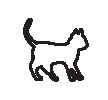
\includegraphics[width=350pt, height=200pt]{chapters/chapter1/figures/cat.eps}
%%\centerline{\epsfig{/Chapters/chapter1/figures/cat.eps,width=.8\textheight,height=.4\textwidth}}
\caption[List of figure caption goes here]{Figure caption goes here.}
\end{figure}



\begin{figure}[htb]
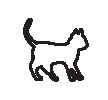
\includegraphics[width=200pt, height=200pt]{chapters/chapter1/figures/cat}
%%\centerline{\epsfig{figure=cat.eps,width=.5\textheight,height=.4\textwidth}}
\caption[Short figure caption]{Figure caption goes here. Figure caption goes here.
Figure caption goes here. Figure caption goes here. Figure caption goes here.
Figure caption goes here.}
\end{figure}





\begin{figure}
\begin{center}
\subfigure[\label{f8a}]{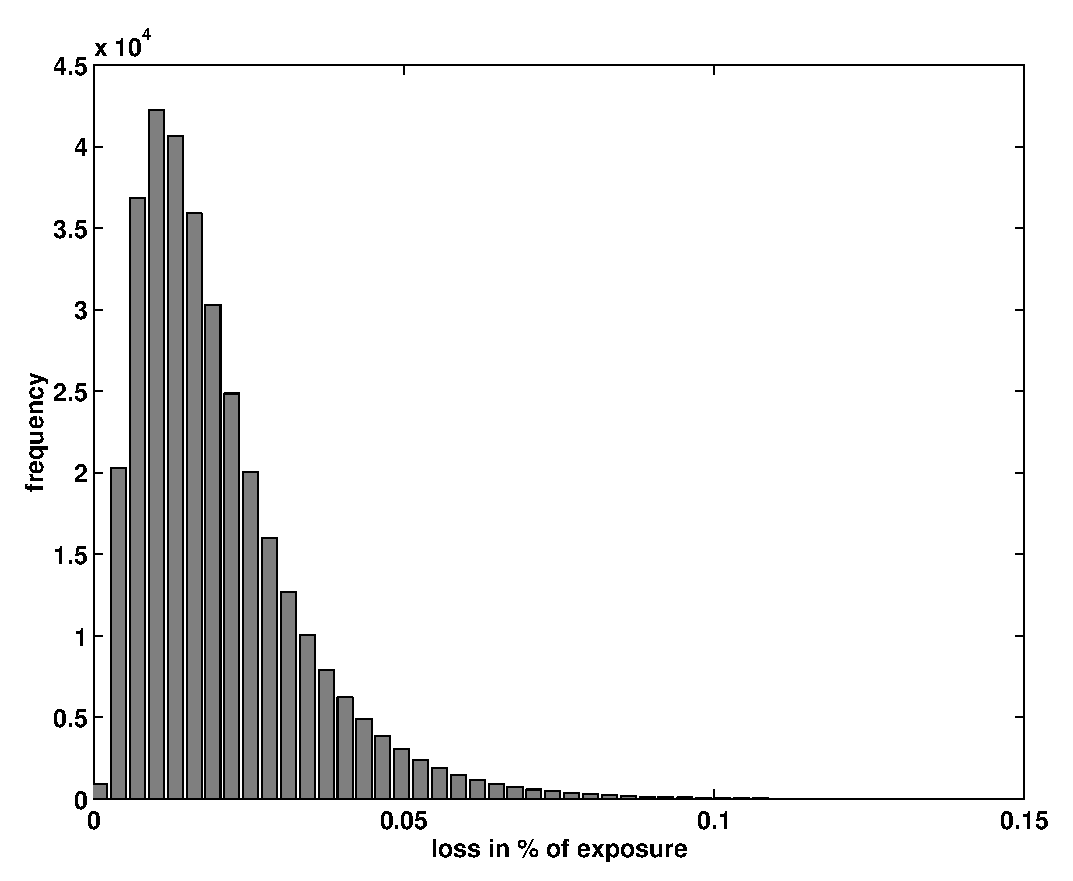
\includegraphics[angle=90,width=7cm,height=7cm,angle=-90]{chapters/chapter1/figures/Histogram.eps}}
\subfigure[\label{f8b}]{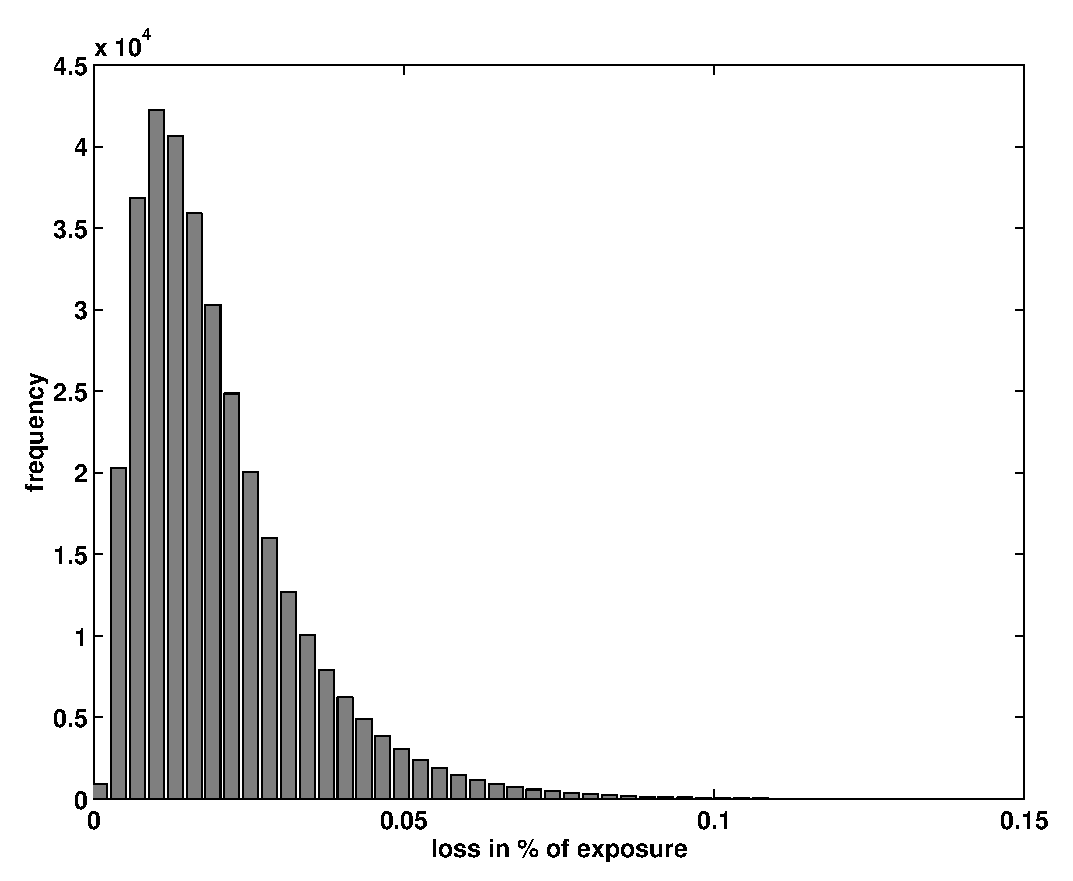
\includegraphics[angle=90,width=7cm,height=7cm,angle=-90]{chapters/chapter1/figures/Histogram.eps}}
\end{center}
\caption[The bar charts depict the different risk contributions]{The bar charts depict the different risk contributions (top: 99\% quantile, bottom: 99.9\% quantile) of the business areas of a bank. The black bars
are based on a Var/Covar approach, the white ones correspond to shortfall risk.}
\end{figure}

\subsubsection{H3 A component part }
A component part for an electronic item is
manufactured at one of three \cite{mardia1979ma} different factories, and then delivered to
the main assembly line.Of the total number supplied, factory A supplies
50\%, factory B 30\%, and factory C 20\%. Of the components
manufactured at factory A, 1\% are faulty and the corresponding
proportions for factories B and C are 4\% and 2\% respectively. A
component is picked at random from the assembly line. What is the
probability that it is faulty?


A fundamental notion \cite{yao2002can} is that of a\index{subspace}\index{vector
space!subspace of} subspace of $F^n$. Let $V$ be a nonempty subset of
$F^n$. Then $V$ is a {\it subspace} of $F^n$ provided $V$ is closed
under vector addition and scalar multiplication, that is,
\begin{enumerate}
\item[\rm (a)] For all $u$ and $v$ in $V$, $u+v$ is
also in $V$.
\item[\rm (b)] For all $u$ in $V$ and $c$ in $F$, $cu$ is
in $V$.
\end{enumerate}
Let $u$ be in the subspace $V$. Because $0u=0$,
it follows that the zero vector is in $V$. Similarly, $-u$ is in $V$
for all $u$ in $V$. A simple example of a subspace of $F^n$ is the set
of all vectors $(0,a_2,\ldots,a_n)$ with first coordinate equal to 0.
The zero vector itself is a subspace.

\begin{definition}\label{1def:linearcomb}{\rm
Let $u^{(1)},u^{(2)},\ldots,u^{(m)}$ be vectors in $F^n$, and let
$c_1,c_2,\ldots,c_m$ be scalars. Then the vector
\[c_1u^{(1)}+c_2u^{(2)}+\cdots+c_mu^{(m)}\]
is called a {\it linear combination} \index{linear combination} of $u^{(1)},u^{(2)},\ldots,u^{(m)}$.
If $V$ is a subspace of $F^n$, then $V$ is closed under vector addition and
scalar multiplication, and it follows easily by induction that a
linear combination of vectors in $V$ is also a vector in $V$. Thus
{\it subspaces
are closed under linear combinations}; in fact, this can be taken as the
defining property of subspaces.
The vectors $u^{(1)},u^{(2)},\ldots,u^{(m)}$ {\it span} $V$ \index{spanning set}
(equivalently, form a {\it spanning set} of $V$) provided every vector in
$V$
is a linear combination of $u^{(1)},u^{(2)},\ldots,u^{(m)}$. The zero
vector can be written as a linear combination of
$u^{(1)},u^{(2)},\ldots,u^{(m)}$ with all scalars equal to 0; this is a
{\it trivial linear combination}.\index{linear combination!trivial} The vectors
$u^{(1)},u^{(2)},\ldots,u^{(m)}$ are {\it linearly dependent} provided
there are scalars $c_1,c_2,\ldots,c_m$, not all of which are zero, such
that
\[c_1u^{(1)}+c_2u^{(2)}+\cdots+c_mu^{(m)}=0,\]
that is, the zero vector can be written as a {\it nontrivial linear \index{linear combination!nontrivial}
combination} of $u^{(1)},u^{(2)},\ldots,u^{(m)}$.
For example, the vectors $(1,4), (3,-1)$, and $(3,5)$ in $\Re^2$ are
linearly
dependent since
\[3(1,4)+1(3,-2)-2(3,5)=(0,0).\] Vectors are {\it linearly independent} provided  they are not linearly dependent.\index{linearly independent}
The vectors
$u^{(1)},u^{(2)},\ldots,u^{(m)}$ are a {\it basis} \index{basis} of $V$ provided they are
linearly independent and span $V$.
By an {\it ordered basis} \index{basis!ordered} we mean a basis in which the vectors of the basis are listed
in a specified order; to indicate that we have an ordered basis we write
$(u^{(1)},u^{(2)},\ldots,u^{(m)})$.
A spanning set $S$ of $V$ is a \index{spanning set!minimal} {\it minimal spanning set of $V$} provided that
each set
of vectors obtained from $S$ by removing a vector is not a spanning set
for $V$.
A linearly independent set $S$ of vectors of $V$ is a {\it maximal linearly \index{linearly independent!maximal}
independent set of vectors of $V$} provided that for each vector $w$ of
$V$ that
is not in $S$, $S\cup\{w\}$ is  linearly dependent (when this happens,
$w$ must be  a linear combination of the vectors in
$S$).\hfill{$\Box$}
}\end{definition}

In addition to matrix addition, subtraction, and multiplication, there is
one additional operation that we define now. It's perhaps the simplest of
them all. Let $A=[a_{ij}]$ be an $m$ by $n$ matrix and let $c$ be a
number \cite{hyvarinen2001ica}. Then the matrix $c\cdot A$, or simply $cA$, is the $m$ by $n$
matrix obtained by multiplying each entry of $A$ by $c$:
\[c A=[ca_{ij}].\]\index{matrix!scalar multiplication} \index{matrix!scalar multiple of}
The matrix $c A$ is called a {\it scalar multiple} of $A$.

\begin{VT1}

\VH{Think About It...}

Commonly thought of as the first modern computer, ENTAC was built in 1944. It took up more space than an 18-wheeler's
tractor trailer and weighed more than 17 Chevrolet Camaros. It consumed 140,000 watts of electricity while executing
up to 5,000 basic arithmetic operations per second. One of today's popular microprocessors, the 486, is built on a
tiny piece of silicon about the size of a dime.

\VT
With the continual expansion of capabilities, computing power will eventually exceed the capacity for human
comprehension or human control.

\VTA{The Information Revolution}{Business Week}
\end{VT1}


\section{Glossary}
\begin{Glossary}
\item[360 Degree Review] Performance review that includes feedback from superiors, peers, subordinates, and clients.
\item[Abnormal Variation] Changes in process performance that cannot be accounted for by typical day-to-day variation. Also referred to as
non-random variation.
\item[Acceptable Quality Level (AQL)] The minimum number of parts that must comply with quality standards, usually stated as a percentage.
\item[Activity] The tasks performed to change inputs into outputs.
\item[Adaptable] An adaptable process is designed to maintain effectiveness and efficiency as requirements change. The process is
deemed adaptable when there is agreement among suppliers, owners, and customers that the process will meet
requirements throughout the strategic period.
\end{Glossary}




\chapter{Descripción de IntroProg}

En esta sección se explica con más detalle lo que es el lenguaje y sus capacidades.
%---------------------------------------------------------------------------------------
\section{Introducción a IntroProg}\label{intro}

Es un lenguaje de programación sencillo con un enfoque hacia data science. La idea del lenguaje es permitir a personas interesadas en programar a experimentar con proyectos sencillos de ciencia de datos.

IntroProg permite al usuario aprender sobre la lógica de programación, permitiendo que el usuario pueda utilizar estructuras de decisión y estructuras de repetición. También permite que los usuarios experimenten un poco con funciones estadísticas, como generar números que pertenecen a distintas distribuciones de probabilidad como la función Normal, Exponencial, Poisson y Geométrica. Además, permite que los usuarios puedan crear gráficas de los datos con los que trabajan.


%---------------------------------------------------------------------------------------
\section{Características Principales}
IntroProg cuenta con múltiples características que la mayoría de los lenguajes de programación cuentan. Estos van de estructuras de control y flujo hasta el manejo de funciones y arreglos.
Como IntroProg es un lenguaje de aprendizaje puede ser un poco restrictivo, pero en esta sección se va a describir con un poco más de detalle en que consta cada una de las características del lenguaje, incluyendo las funciones especiales.

\FloatBarrier

\subsection{Estructura general de un programa de IntroProg}
Los archivos del lenguaje son archivos de texto con terminación \emph{itp}. Para empezar a escribir un programa en IntroProg primero se escribe la palabra clave \emph{programa} seguido por el nombre del programa. Después entre corchetas se escribe las declaraciones de variables, seguida por las declaraciones de funciones, seguido por la función principal. La función principal es la parte del código que se ejecuta primero.

\begin{figure}[!htbp]
    \centering
    
    \begin{lstlisting}
        programa pelos{
            // Primero las variables globales
            entero x;
            bool bo;
            // El codigo principal del programa
            principal funcion {
                // Variables locales a principal
                entero x,y;
            }{
                x = 10;
                y = 2;
                x = x*y;
                imprimir(x);
            }
        }
    \end{lstlisting}
    \caption{Ejemplo de la estructura de un programa de IntroProg}
\end{figure}
\FloatBarrier

Es importante mencionar que un programa puede o no tener una declaración de variables globales y declaración de funciones. Esto dependerá de las necesidades del programador cuando construya su código.

\begin{figure}[!htbp]
    \centering
    
    \begin{lstlisting}
        programa holaMundo { 
	    principal funcion {} {
		    imprimir("Hola Mundo!!!!");
	    } 
    }
    \end{lstlisting}
    \caption{Ejemplo de un programa sin declaración de variables ni declaración de funciones}
\end{figure}
\FloatBarrier

Aunque parezca un poco confuso al principio, se van a ir explicando parte por parte la estructura y funcionalidades del lenguaje en las siguientes secciones.

\subsection{Variables y la declaración de variables}

Para poder programar primero se necesitan utilizar variables. Las variables son representaciones de información que pueden ser modificadas por el programador para calcular y modelar información. Las variables en IntroProg están representadas por un identificador que es una serie de letras, guiones y números. Los identificadores siempre deben de empezar con una letra.

Para declarar una variable no solo es importante tener un buen identificador sino también hay que indicar el tipo de la variable. En IntroProg se manejan cuatro tipos de variables los cuales son:

\begin{itemize}
    \item Enteros: Números enteros (ej. 1,2,3).  Estos son representados por la palabra clave \emph{entero}
    \item Flotantes: Números Flotantes o decimales (ej. 3.1416), representados por la palabra clave \emph{flotante} 
    \item Caracteres: Letras (ej. 'a', 'b'). Estas estan representadas por la palabra clave \emph{char}
    \item Booleanos: Valores Booleanos (ej. Verdadero o falso). Esta representados por la palabra clave \emph{bool}
\end{itemize}

\begin{figure}[!htbp]
    \centering
    
    \begin{lstlisting}
        entero una_Variable_1;
    \end{lstlisting}
    \caption{Ejemplo de una declaración de variable}
\end{figure}
\FloatBarrier
Las declaraciones solo se pueden hacer en los lugares apropiados en el programa para las declaraciones. Estos son el espacio de variables globales que se encuentra directamente después de la primera corcheta del programa, y en las corchetas de declaración de variables locales los cuales se encuentran después de los nombres de funciones.

Los programas cuentan con dos tipos de alcances de variables. Las variables globales, las cuales pueden ser accesados por todas las funciones del programa y las variables locales que solo pueden ser accesados por las funciones en las que fueron declaradas.

\subsection{Expresiones, Imprimir, Asignación y Comentarios}

Solo declarar las variables no es suficiente para hacer programas. Por ello IntroProg cuenta con una serie de estatutos básicos que son utilizados para realizar operaciones con las variables declaradas. Primero para poder asignarles información a las variables se tiene que hacer una asignación. Esto se logra utilizando el símbolo de \emph{\=}. Para asignar valores a variables primero se tiene que escribir el identificador de la variable seguido por el símbolo \emph{\=} seguido del valor que se le quiere asignar.

\begin{figure}[!htbp]
    \centering
    
    \begin{lstlisting}
        una_Variable_1 = 10;
        // Tambien se le pueden asignar 
        // el valor de otra variable
        una_Variable_1 = x; 
    \end{lstlisting}
    \caption{Ejemplo de asignación}
\end{figure}
\FloatBarrier
Hay que tomar en consideración que solo se le pueden asignar valores a las variables que sean del tipo de la variable. En caso de que se le intente asignar un valor a la variable que no sea de su tipo, IntroProg va a intentar convertir el valor que va a ser asignado al tipo de la variable. Si no puede hacerlo el compilador va a levantar un error.

Ya con valores definidos se pueden empezar a hacer expresiones. Las expresiones en IntroProg son como las expresiones de matemáticas. Estas hacen una operación sobre las variables y constantes y generan un resultado. Estos resultados pueden ser guardados en otras variables.

\begin{figure}[!htbp]
    \centering
    
    \begin{lstlisting}
        una_Variable_1 = 10 * una_Variable_1 + 1;

    \end{lstlisting}
    \caption{Ejemplo de asignación con expresiones}
\end{figure}
\FloatBarrier

IntroProg sigue la siguiente jerquía de operaciones:
\begin{itemize}
    \item Parentesis : Simpre va a hacer primero lo que hay entre parentesis
    \item Negativos/Positivos: Primero se hace negativo o positivo el valor de la variable o constante (ej. -1, +x)
    \item Multiplicaciones/Divisiones : Operaciones de multiplicación y División
    \item Sumas/Restas : Operaciones de sumas y restas
    \item Relacionales : Operaciones relacionales, las cuales son mayor (\emph{>}), menor (\emph{<}), igual (\emph{==}), mayor o igual (\emph{>=}), menor o igual (\emph{<=}) y diferente (\emph{!=})
    \item Lógicas : Operaciones Lógicas como \emph{o (||)} e \emph{y (\&\&)}
\end{itemize}

Es importante mencionar que todos los estatutos o expresiones que se hagan en IntroProg deben de terminar en un punto y coma. De otra manera el compilador va a marcar error.

Pero no solo es necesario hacer operaciones, también es importante saber el resultado de las operaciones. Para poder ver estos resultados es importante poder imprimir a pantalla los valores de las variables. Por eso IntroProg provee el estatuto de \emph{imprimir} el cual permite imprimir a consola el valor de alguna variable o expresión. Para usar este estatuto se tiene que usar la palabra clave \emph{imprimir} seguida por todos los elementos a imprimir separados por comas.

\begin{figure}[!htbp]
    \centering
    
    \begin{lstlisting}
        una_Variable_1 = 10 * una_Variable_1 + 1;
        imprimir(una_Variable,10);

    \end{lstlisting}
    \caption{Ejemplo de impresión}
\end{figure}
\FloatBarrier



Este estatuto también puede manejar el uso de constantes de cadenas. Las constantes de cadenas son oraciones o palabras que estan entre comillas. Esto puede ser util para organizar bien la información cuando se despliega en pantalla.

\begin{figure}[!htbp]
    \centering
    
    \begin{lstlisting}
        una_Variable_1 = 10 * una_Variable_1 + 1;
        imprimir("Esto es una cadena : ",una_Variable,10);

    \end{lstlisting}
    \caption{Ejemplo del uso de cadenas en impresión}
\end{figure}
\FloatBarrier


Finalmente IntroProg cuenta con un estatuto especial que puede ayudar a los programadores a organizar su códgio. Este estatuto es el comentario. El comentario se escribe como dos diagonales seguido de lo que el programador quiera escribir. Todo lo que siga después de las diagonales va a ser ignorado por el compilador.

\begin{figure}[!htbp]
    \centering
    
    \begin{lstlisting}
        una_Variable_1 = 10 * una_Variable_1 + 1;
        imprimir(una_Variable,10); // el comentario puede ser lo que sea
        // El compilador ignora esta linea
        // Y no casua errores

    \end{lstlisting}
    \caption{Ejemplo de Comentarios}
\end{figure}
\FloatBarrier

\subsection{Condiciones}
Las estructuras de control más comúnmente utilizadas. En la mayoría de los lenguajes son reconocido como la instrucción o palabra clave \emph{if}. En IntroProg esta estructura está presente bajo el nombre de \emph{si}, y como su contraparte en C/C++ funciona de manera similar.
\subsubsection{Estructura si}
La estructura \emph{si} está compuesta por la palabra clave seguida de una expresión entre paréntesis. Después de este paréntesis se escribe un bloque de código entre corchetas. El comportamiento de si es el siguiente.
 \emph{Si} recibe una expresión booleana entre paréntesis y si la expresión resulta en verdadero ejecuta el código que se encuentra en los corchetes próximos a la estructura. Si la expresión es falsa se salta a la primera línea de código que sigue después de las corchetas.

\begin{figure}[!htbp]
    \centering
    
    \begin{lstlisting}
        si(expresion){
            //Codigo a ejecutar en verdadero
        }
        //Continua codigo
    \end{lstlisting}
    \caption{Ejemplo de \emph{si}}
\end{figure}
\FloatBarrier
\subsubsection{Estructura si-sino}
Similar a sus contrapartes IntroProg también cuenta con la estructura de \emph{if-else}. En IntroProg esta estructura se escribe con las palabras clave \emph{si} y \emph{sino}. Su funcionamiento es el siguiente. Como un \emph{si} regular, primero se evalúa la expresión que se encuentra entre paréntesis enfrente de la palabra clave, si es verdadero ejecuta el código entre las corchetas seguidas de la expresión. En caso de que la condición sea falsa se salta a ejecutar las corchetas después de la palabra clave \emph{sino}.

\begin{figure}[!htbp]
    \centering
    
    \begin{lstlisting}
        si(expresion){
            //Codigo a ejecutar en verdadero
        }sino{
            //Codigo a ejecutar en falso
        }
        //Continua codigo
    \end{lstlisting}
    \caption{Ejemplo de \emph{si-sino}}
\end{figure}
\FloatBarrier

\FloatBarrier
\subsection{Bucles}

Los bucles son una de las estructuras de flujo esenciales de los lenguajes de programación. Y como todos los lenguajes, IntroProg también cuenta con formas de representar estas estructuras. En IntroProg hay dos formas de hacer bucles. La primera estructura es \emph{mientras}, el cual es muy similar a su contraparte de C/C++ \emph{while}. La segunda estructura es \emph{por} el cual es similar a su contraparte de C/C++ \emph{for}.
\\
\subsubsection{Estructura Mientras}
La estructura de \emph{mientras} consta de la palabra clave seguida de una expresión entre paréntesis y un bloque de código entre corchetas. Lo que va a hacer es repetir el bloque de código mientras que la expresión que se encuentra entre paréntesis enfrente del \emph{mientras}. Si la expresión resulta en falso se salta a la siguiente línea de código después de la estructura.

\begin{figure}[!htbp]
    \centering
    
    \begin{lstlisting}
        mientras(expresion){
            //Codigo a repetir mientras sea verdadero
        }
        // Codigo continua aqui
    \end{lstlisting}
    \caption{Ejemplo de \emph{mientras}}
\end{figure}
\FloatBarrier

\subsubsection{Estructura Por}
La segunda estructura de flujo de IntroProg es la estructura \emph{por}, la cual es similar a su contraparte \emph{for} en el lenguaje C/C++. La estructura consta de la palabra \emph{por} seguida por una asignación, una expresión a evaluar y una segunda asignación indicando el paso a seguir después de cada ciclo encerrado entre un paréntesis. Seguido de este paréntesis sigue un bloque de código entre corchetas el cual va a ser ejecutado mientras que la expresión del \emph{por} sea verdadera.

\begin{figure}[!htbp]
    \centering
    
    \begin{lstlisting}
        por(asignacion; expresion; asignacion;){
            //Codigo a repetir
        }
        //Codigo continua
    \end{lstlisting}
    \caption{Ejemplo de \emph{por}}
\end{figure}
\FloatBarrier

El \emph{por} también se puede escribir sin la primera asignación, asumiendo que la variables utilizadas en el paso y la expresión estén declaradas.


\begin{figure}[!htbp]
    \centering
    
    \begin{lstlisting}
        por(; expresion; asignacion;){
            //Codigo a repetir
        }
        //Codigo continua
    \end{lstlisting}
    \caption{Ejemplo de \emph{por} sin la primera asignación}
\end{figure}

\FloatBarrier
\subsection{Funciones}

Otra parte importante de los lenguajes de programación es la posibilidad de poder romper el código en funciones que cumplen un funcionamiento especifico, definido por el programador. IntroProg estructura sus funciones de la siguiente manera.

\subsubsection{Declaración de función}

Antes de utilizar funciones es importante primero que el usuario declare las funciones. Para ello hay que escribir la declaración de las funciones en el espacio apropiado. En la estructura de un programa de IntroProg las funciones se declaran después de las declaraciones de las variables globales, pero antes de la función principal.

\begin{figure}[!htbp]
    \centering
    
    \begin{lstlisting}
        programa pelos{
            // Primero las variables globales
            entero x;
            bool bo;
            // Aqui van las funciones
            funcion vacio holaMundo(){}{
                imprimir("Hola Mundo!!!");
            }
            // El codigo principal del programa
            principal funcion {
                // Variables locales a principal
                entero x,y;
            }{
                x = 10;
                y = 2;
                x = x*y;
                imprimir(x);
                $holaMundo();
            }
        }
    \end{lstlisting}
    \caption{Ejemplo del lugar donde se declaran las funciones}
\end{figure}
\FloatBarrier

El programador puede declarar una función usando la palabra clave \emph{funcion} seguida por el tipo de función. Después se escribe los parámetros de la función, escritos entre paréntesis denotando el tipo y el identificador del parámetro. Es importante remarcar que una función puede no tener parámetros. Se pueden definir múltiples parámetros separando con comas cada uno de ellos. Después de definir los parámetros se escribe entre corchetas las declaraciones de variables. Si no se planea usar variables locales en la función se puede dejar vació el espacio entre los corchetes. Después de declarar las variables se escribe el bloque de código que debe de ejecutar la función entre corchetas.

\begin{figure}[!htbp]
    \centering
    
    \begin{lstlisting}
        funcion vacio holaMundo(){}{
            imprimir("Hola Mundo!!!");
        }
    \end{lstlisting}
    \caption{Ejemplo de función vacia}
\end{figure}
\FloatBarrier

\begin{figure}[!htbp]
    \centering
    
    \begin{lstlisting}
        funcion entero suma( entero n, entero m){}{
            regresa n * m;
        }
    \end{lstlisting}
    \caption{Ejemplo de función con retorno}
\end{figure}
\FloatBarrier

En IntroProg hay dos tipos de funciones, las funciones vacías y las funciones con retorno. Las funciones vacías sirven solo para ejecutar código que no se esperan que regresen un valor, esto puede ser imprimir el resultado de ciertas variables o hacer cálculos temporales que no se van a utilizar después. Las funciones con retorno son funciones que realizan operaciones y que regresan un resultado. El valor de retorno de estas funciones están indicadas por la palabra clave \emph{regresar} seguida por una expresión el cual su resultado es el que va a ser utilizado. Cabe recalcar que las funciones vacío no pueden tener el estatuto de \emph{regresar}.


\subsubsection{Llamada de función}

Una vez declarada las funciones pueden ser utilizadas como el elemento de una expresión. Esto se logra utilizando el símbolo de dólar (\emph{\$}) seguido por el nombre de la función, seguido por un paréntesis con expresiones separados por comas, representando los argumentos. Si la función no tiene argumentos se dejan los paréntesis vacíos.

\begin{figure}[!htbp]
    \centering
   
    \begin{lstlisting}
            principal funcion {
                // Variables locales a principal
                entero x,y;
            }{
                x = 10;
                y = 2;
                x = $suma(x, x*y);
                imprimir(x);
                $holaMundo();
            }
    \end{lstlisting}
     \caption{Ejemplo del lugar donde se declaran las funciones}
\end{figure}
\FloatBarrier
\subsubsection{Llamadas recursivas en funciones}

IntroProg también soporta el uso de funciones recursivas. Esto se puede lograr haciendo la llamada de la misma función dentro de su declaración. Esto puede ser útil para resolver ciertos problemas de programación.

\begin{figure}[!htbp]
    \centering
    
    \begin{lstlisting}
        funcion entera factorial ( entero  n) {}{
            regresa n * $factorial(n-1);
        } 
    \end{lstlisting}
    \caption{Ejemplo de función recursiva}
\end{figure}


\FloatBarrier
\subsection{Arreglos, Matrices y Cubos}

En IntroProg las variables no solo se pueden usar para guardar solo un valor. Se pueden declarar arreglos los cuales pueden tener múltiples valores dependiendo de su declaración. Para declarar un arreglo se usa una sintaxis muy similar a la declaración simple. La declaración de un arreglo se da escribiendo primero el tipo de la variable, seguido por su identificador, seguido del tamaño del arreglo encerrado entre corchetas cuadradas.\\

\begin{figure}[!htbp]
    \centering
    
    \begin{lstlisting}
        entero arreglo [10]; // Un arreglo de 10 valores

    \end{lstlisting}
    \caption{Ejemplo de la declaración de un arreglo}
\end{figure}
\FloatBarrier


Para poder accesar a uno de los valores que tiene el arreglo se puede llamar en una expresión de la siguiente manera. Se escribe el nombre del arreglo seguido de la posición del valor entre corchetas cuadradas. Las posiciones en IntroProg se empiezan a contar desde el 0 hasta el número entero anterior al tamaño.\\

\begin{figure}[!htbp]
    \centering
    
    \begin{lstlisting}
        arreglo[0] = 10; // primera posicion del arreglo
        arreglo[9] = 2003; // Ultima posicion del arreglo
        //Tambien se pueden usar para operaciones
        arreglo[2] = arreglo[0] * arreglo[9];

    \end{lstlisting}
    \caption{Ejemplo de la llamada de un arreglo}
\end{figure}
\FloatBarrier
Los arreglos en IntroProg también se les pueden asignar valores de manera directa a todas las casillas del arreglo. Esto se puede lograr listando los valores entre corchetas cuadradas y separando los valores entre comas.

\begin{figure}[!htbp]
    \centering
    
    \begin{lstlisting}
        arreglo = [1,2,3,4,5,6,7,8,9,10]

    \end{lstlisting}
    \caption{Ejemplo de una asignación textual a un arreglo}
\end{figure}
\FloatBarrier
\subsubsection{Matrices y Cubos}
IntroProg no solo maneja arreglos sino también maneja matrices y cubos. La forma de interactuar con ellos es muy similar a los arreglos. Solo se necesita hacer lo mismo que se hace con un arreglo solo que en vez de utilizar solo un set de corchetas cuadradas se usan la cantidad de corchetas cuadradas a las dimensiones a utilizar. Es importante mencionar que IntroProg solo maneja hasta cubos y no permite crear variables con más dimensiones.

\begin{figure}[!htbp]
    \centering
    
    \begin{lstlisting}
        entero mat[3][3];
        entero cubo[2][2][2];

    \end{lstlisting}
    \caption{Ejemplo de la declaración de una matriz y un cubo}
\end{figure}
\FloatBarrier

\begin{figure}[!htbp]
    \centering
    
    \begin{lstlisting}
        mat[0][0] = 10;
        cubo[0][1][1] = 10;

    \end{lstlisting}
    \caption{Ejemplo de la llamada de una matriz y un cubo}
\end{figure}
\FloatBarrier

\begin{figure}[!htbp]
    \centering
    
    \begin{lstlisting}
        mat = [[1,2,3],[4,5,6],[7,8,9]];
        cubo = [[[1,2],[3,4]],[[5,6],[7,8]]];

    \end{lstlisting}
    \caption{Ejemplo de una asignación textual de una matriz y un cubo}
\end{figure}
\FloatBarrier






\FloatBarrier
\subsection{Funciones Especiales}

IntroProg también cuenta con una serie de funciones especiales que pueden ser utilizadas en cualquier programa. Estas funciones tienen un enfoque hacia estadística, y le permiten a los usuarios hacer programas más complejos. Estas funciones son:

\begin{itemize}
    \item \$leer() : Regresa la lectura capturada de consola
    \item \$modulo(flotante a, flotante b): Regresa el resultado de a\%b
    \item \$suma(flotante a[]): Suma todos los elementos de un arreglo y regresa sus resultados
    \item \$raiz(flotante a): Regresa el flotante resultante de la raíz de a
    \item \$exp(flotante a): Regresa la exponencial de e\^a
    \item \$elevar(flotante a, flotante b): Regresa el resultado de a\^b
    \item \$techo(flotante a): Regresa un flotante a redondeado para arriba
    \item \$piso(flotante a): Regresa un flotante a redondeado para abajo
    \item \$cos(flotante a): Regresa el coseno de a
    \item \$sen(flotante a): Regresa el seno de a
    \item \$tan(flotante a): Regresa la tangente de a
    \item \$cotan(flotante a): Regresa la cotangente de a
    \item \$sec(flotante a): Regresa la secante de a
    \item \$cosec(flotante a): Regresa la cosecante de a
    \item \$log(flotante a): Regresa el logaritmo natural de a
    \item \$minimo(flotante a[]): Regresa el valor más chico en el vector a
    \item \$maximo(flotante a[]): Regresa el valor máximo de a
    \item \$redondear(flotante a): Regresa un flotante a redondeado 
    \item \$productoPunto(flotante a[], flotante b[]): Regresa el producto punto entre los vectores de entrada a y b
    \item \$media(flotante a[]): Regresa la media de a
    \item \$mediana(flotante a[]): regresa la mediana de a
    \item \$moda(flotante a[]): Regresa el elemento con la moda más alta de a
    \item \$varianza(a): Regresa la varianza de a
    \item \$percentil(flotante a[], flotante q): Regresa el valor en el que se encuentran q% de los valores en a
    \item \$aleatorio(flotante min, flotante max): Regresa un número flotante aleatorio entre los rangos de argumentos mínimos y máximos
    \item \$wilcoxon(flotante x[]): Realiza la prueba de Wilcoxon en la serie de datos en x
    \item \$wilcoxonComp(flotante x[], flotante y[]):Realiza la prueba de Wilcoxon se realiza la prueba sobre los datos x y y.
    \item \$regresionSimple(flotante x[], flotante y[], flotante xi): Dado un set de x y y se usará regresión lineal simple para encontrar f(xi) y se regresara ese valor
    \item \$normal(flotante media, flotante desv): Regresa un número escalar que pertenezca a la distribución normal dado los parámetros
    \item \$poisson(flotante lambda): Regresa un número aleatorio de la distribución Poisson con la lambda dada
    \item \$dexponencial(flotante beta): Regresa un número aleatorio de la distribución Exponencial correspondiente a la beta (o 1/Lambda) dada.
    \item \$dgeometrica(flotante exito): Te regresa un valor con la distribución geométrica con la probabilidad de exito dada. 
    \item \$histograma(flotante x[], flotante rango): Genera un histograma a partir de los datos en el vector de x con un rango entre los datos de rango.
    \item \$diagramadecaja(flotante x[]): Genera un diagrama de caja y bigotes de los datos en en x
    \item \$grafDispersion(flotante x[], flotante y[]): Genera un gráfico de dispersión con los valores de ‘x’ y ‘y’
\end{itemize}

Para llamar a una función especial se usa la misma sintaxis que una función normal.

\begin{figure}[!htbp]
    \centering
    
    \begin{lstlisting}
            x = $aleatorio(1,100);
    \end{lstlisting}
    \caption{Ejemplo del uso de funcinoes especiales}
\end{figure}
\FloatBarrier

\FloatBarrier

%---------------------------------------------------------------------------------------

\section{Listado de errores}
El compilador y la máquina virtual manejan distintos tipos de errores que pueden suceder cuando se hace un programa. Como el lenguaje está diseñado para ser un punto de entrada a la programación se intentó cubrir la mayor cantidad de errores de programación comunes y se agregaron mensajes de error apropiados a la situación del error. Estos mensajes de error tratan de explicar de una manera clara cuál es la situación que causo el error al usuario.\\

Los errores que se pueden detectar durante compilación son los siguientes:
\begin{itemize}
    \item Doble declaración de variables
    \item El uso de variables no declaradas.
    \item Errores de sintaxis. Esto incluye identificadores y palabras reservadas mal escritas, estatutos mal escritos entre otros errores de sintaxis.
    \item Número de parámetros incorrectos
    \item Asignación incorrecta de parámetros, si el valor pasado como parámetro no se puede convertir a al tipo del parámetro el compilador levanta un error.
    \item Operaciones con funciones vacías, el compilador no permite el uso de funciones vacías en expresiones
    \item Retornos en funciones vacías, El compilador levanta errores cuando detecta un retorno cuando hay retornos en funciones vacías
    \item No permitir el nombre de funciones y palabras reservadas como identificadores.
\end{itemize}

Los errores que puede detectar la máquina virtual son la siguiente:
\begin{itemize}
    \item Operaciones con variables sin valor. Si se intenta realizar operaciones con variables las cuales no cuentan con un valor se levanta un error y se le indica al usuario cuál fue el posible error.
    \item Detectar si los subíndices del arreglo se salen del espacio definido por el arreglo. Similarmente detecta cuando el arreglo se sale de los límites del arreglo e indica al usuario mediante un mensaje de error lo que sucedió.
    \item Lectura incorrecta. Cuando se utiliza la lectura y se mete un valor que no es válido para lectura.
\end{itemize}




%\part{Descripción del lenguaje}
%\chapter{Descripción de IntroProg}

En esta sección se explica con más detalle lo que es el lenguaje y sus capacidades.
%---------------------------------------------------------------------------------------
\section{Introducción a IntroProg}\label{intro}

Es un lenguaje de programación sencillo con un enfoque hacia data science. La idea del lenguaje es permitir a personas interesadas en programar a experimentar con proyectos sencillos de ciencia de datos.

IntroProg permite al usuario aprender sobre la lógica de programación, permitiendo que el usuario pueda utilizar estructuras de decisión y estructuras de repetición. También permite que los usuarios experimenten un poco con funciones estadísticas, como generar números que pertenecen a distintas distribuciones de probabilidad como la función Normal, Exponencial, Poisson y Geométrica. Además, permite que los usuarios puedan crear gráficas de los datos con los que trabajan.


%---------------------------------------------------------------------------------------
\section{Características Principales}
IntroProg cuenta con múltiples características que la mayoría de los lenguajes de programación cuentan. Estos van de estructuras de control y flujo hasta el manejo de funciones y arreglos.
Como IntroProg es un lenguaje de aprendizaje puede ser un poco restrictivo, pero en esta sección se va a describir con un poco más de detalle en que consta cada una de las características del lenguaje, incluyendo las funciones especiales.

\FloatBarrier

\subsection{Estructura general de un programa de IntroProg}
Los archivos del lenguaje son archivos de texto con terminación \emph{itp}. Para empezar a escribir un programa en IntroProg primero se escribe la palabra clave \emph{programa} seguido por el nombre del programa. Después entre corchetas se escribe las declaraciones de variables, seguida por las declaraciones de funciones, seguido por la función principal. La función principal es la parte del código que se ejecuta primero.

\begin{figure}[!htbp]
    \centering
    
    \begin{lstlisting}
        programa pelos{
            // Primero las variables globales
            entero x;
            bool bo;
            // El codigo principal del programa
            principal funcion {
                // Variables locales a principal
                entero x,y;
            }{
                x = 10;
                y = 2;
                x = x*y;
                imprimir(x);
            }
        }
    \end{lstlisting}
    \caption{Ejemplo de la estructura de un programa de IntroProg}
\end{figure}
\FloatBarrier

Es importante mencionar que un programa puede o no tener una declaración de variables globales y declaración de funciones. Esto dependerá de las necesidades del programador cuando construya su código.

\begin{figure}[!htbp]
    \centering
    
    \begin{lstlisting}
        programa holaMundo { 
	    principal funcion {} {
		    imprimir("Hola Mundo!!!!");
	    } 
    }
    \end{lstlisting}
    \caption{Ejemplo de un programa sin declaración de variables ni declaración de funciones}
\end{figure}
\FloatBarrier

Aunque parezca un poco confuso al principio, se van a ir explicando parte por parte la estructura y funcionalidades del lenguaje en las siguientes secciones.

\subsection{Variables y la declaración de variables}

Para poder programar primero se necesitan utilizar variables. Las variables son representaciones de información que pueden ser modificadas por el programador para calcular y modelar información. Las variables en IntroProg están representadas por un identificador que es una serie de letras, guiones y números. Los identificadores siempre deben de empezar con una letra.

Para declarar una variable no solo es importante tener un buen identificador sino también hay que indicar el tipo de la variable. En IntroProg se manejan cuatro tipos de variables los cuales son:

\begin{itemize}
    \item Enteros: Números enteros (ej. 1,2,3).  Estos son representados por la palabra clave \emph{entero}
    \item Flotantes: Números Flotantes o decimales (ej. 3.1416), representados por la palabra clave \emph{flotante} 
    \item Caracteres: Letras (ej. 'a', 'b'). Estas estan representadas por la palabra clave \emph{char}
    \item Booleanos: Valores Booleanos (ej. Verdadero o falso). Esta representados por la palabra clave \emph{bool}
\end{itemize}

\begin{figure}[!htbp]
    \centering
    
    \begin{lstlisting}
        entero una_Variable_1;
    \end{lstlisting}
    \caption{Ejemplo de una declaración de variable}
\end{figure}
\FloatBarrier
Las declaraciones solo se pueden hacer en los lugares apropiados en el programa para las declaraciones. Estos son el espacio de variables globales que se encuentra directamente después de la primera corcheta del programa, y en las corchetas de declaración de variables locales los cuales se encuentran después de los nombres de funciones.

Los programas cuentan con dos tipos de alcances de variables. Las variables globales, las cuales pueden ser accesados por todas las funciones del programa y las variables locales que solo pueden ser accesados por las funciones en las que fueron declaradas.

\subsection{Expresiones, Imprimir, Asignación y Comentarios}

Solo declarar las variables no es suficiente para hacer programas. Por ello IntroProg cuenta con una serie de estatutos básicos que son utilizados para realizar operaciones con las variables declaradas. Primero para poder asignarles información a las variables se tiene que hacer una asignación. Esto se logra utilizando el símbolo de \emph{\=}. Para asignar valores a variables primero se tiene que escribir el identificador de la variable seguido por el símbolo \emph{\=} seguido del valor que se le quiere asignar.

\begin{figure}[!htbp]
    \centering
    
    \begin{lstlisting}
        una_Variable_1 = 10;
        // Tambien se le pueden asignar 
        // el valor de otra variable
        una_Variable_1 = x; 
    \end{lstlisting}
    \caption{Ejemplo de asignación}
\end{figure}
\FloatBarrier
Hay que tomar en consideración que solo se le pueden asignar valores a las variables que sean del tipo de la variable. En caso de que se le intente asignar un valor a la variable que no sea de su tipo, IntroProg va a intentar convertir el valor que va a ser asignado al tipo de la variable. Si no puede hacerlo el compilador va a levantar un error.

Ya con valores definidos se pueden empezar a hacer expresiones. Las expresiones en IntroProg son como las expresiones de matemáticas. Estas hacen una operación sobre las variables y constantes y generan un resultado. Estos resultados pueden ser guardados en otras variables.

\begin{figure}[!htbp]
    \centering
    
    \begin{lstlisting}
        una_Variable_1 = 10 * una_Variable_1 + 1;

    \end{lstlisting}
    \caption{Ejemplo de asignación con expresiones}
\end{figure}
\FloatBarrier

IntroProg sigue la siguiente jerquía de operaciones:
\begin{itemize}
    \item Parentesis : Simpre va a hacer primero lo que hay entre parentesis
    \item Negativos/Positivos: Primero se hace negativo o positivo el valor de la variable o constante (ej. -1, +x)
    \item Multiplicaciones/Divisiones : Operaciones de multiplicación y División
    \item Sumas/Restas : Operaciones de sumas y restas
    \item Relacionales : Operaciones relacionales, las cuales son mayor (\emph{>}), menor (\emph{<}), igual (\emph{==}), mayor o igual (\emph{>=}), menor o igual (\emph{<=}) y diferente (\emph{!=})
    \item Lógicas : Operaciones Lógicas como \emph{o (||)} e \emph{y (\&\&)}
\end{itemize}

Es importante mencionar que todos los estatutos o expresiones que se hagan en IntroProg deben de terminar en un punto y coma. De otra manera el compilador va a marcar error.

Pero no solo es necesario hacer operaciones, también es importante saber el resultado de las operaciones. Para poder ver estos resultados es importante poder imprimir a pantalla los valores de las variables. Por eso IntroProg provee el estatuto de \emph{imprimir} el cual permite imprimir a consola el valor de alguna variable o expresión. Para usar este estatuto se tiene que usar la palabra clave \emph{imprimir} seguida por todos los elementos a imprimir separados por comas.

\begin{figure}[!htbp]
    \centering
    
    \begin{lstlisting}
        una_Variable_1 = 10 * una_Variable_1 + 1;
        imprimir(una_Variable,10);

    \end{lstlisting}
    \caption{Ejemplo de impresión}
\end{figure}
\FloatBarrier



Este estatuto también puede manejar el uso de constantes de cadenas. Las constantes de cadenas son oraciones o palabras que estan entre comillas. Esto puede ser util para organizar bien la información cuando se despliega en pantalla.

\begin{figure}[!htbp]
    \centering
    
    \begin{lstlisting}
        una_Variable_1 = 10 * una_Variable_1 + 1;
        imprimir("Esto es una cadena : ",una_Variable,10);

    \end{lstlisting}
    \caption{Ejemplo del uso de cadenas en impresión}
\end{figure}
\FloatBarrier


Finalmente IntroProg cuenta con un estatuto especial que puede ayudar a los programadores a organizar su códgio. Este estatuto es el comentario. El comentario se escribe como dos diagonales seguido de lo que el programador quiera escribir. Todo lo que siga después de las diagonales va a ser ignorado por el compilador.

\begin{figure}[!htbp]
    \centering
    
    \begin{lstlisting}
        una_Variable_1 = 10 * una_Variable_1 + 1;
        imprimir(una_Variable,10); // el comentario puede ser lo que sea
        // El compilador ignora esta linea
        // Y no casua errores

    \end{lstlisting}
    \caption{Ejemplo de Comentarios}
\end{figure}
\FloatBarrier

\subsection{Condiciones}
Las estructuras de control más comúnmente utilizadas. En la mayoría de los lenguajes son reconocido como la instrucción o palabra clave \emph{if}. En IntroProg esta estructura está presente bajo el nombre de \emph{si}, y como su contraparte en C/C++ funciona de manera similar.
\subsubsection{Estructura si}
La estructura \emph{si} está compuesta por la palabra clave seguida de una expresión entre paréntesis. Después de este paréntesis se escribe un bloque de código entre corchetas. El comportamiento de si es el siguiente.
 \emph{Si} recibe una expresión booleana entre paréntesis y si la expresión resulta en verdadero ejecuta el código que se encuentra en los corchetes próximos a la estructura. Si la expresión es falsa se salta a la primera línea de código que sigue después de las corchetas.

\begin{figure}[!htbp]
    \centering
    
    \begin{lstlisting}
        si(expresion){
            //Codigo a ejecutar en verdadero
        }
        //Continua codigo
    \end{lstlisting}
    \caption{Ejemplo de \emph{si}}
\end{figure}
\FloatBarrier
\subsubsection{Estructura si-sino}
Similar a sus contrapartes IntroProg también cuenta con la estructura de \emph{if-else}. En IntroProg esta estructura se escribe con las palabras clave \emph{si} y \emph{sino}. Su funcionamiento es el siguiente. Como un \emph{si} regular, primero se evalúa la expresión que se encuentra entre paréntesis enfrente de la palabra clave, si es verdadero ejecuta el código entre las corchetas seguidas de la expresión. En caso de que la condición sea falsa se salta a ejecutar las corchetas después de la palabra clave \emph{sino}.

\begin{figure}[!htbp]
    \centering
    
    \begin{lstlisting}
        si(expresion){
            //Codigo a ejecutar en verdadero
        }sino{
            //Codigo a ejecutar en falso
        }
        //Continua codigo
    \end{lstlisting}
    \caption{Ejemplo de \emph{si-sino}}
\end{figure}
\FloatBarrier

\FloatBarrier
\subsection{Bucles}

Los bucles son una de las estructuras de flujo esenciales de los lenguajes de programación. Y como todos los lenguajes, IntroProg también cuenta con formas de representar estas estructuras. En IntroProg hay dos formas de hacer bucles. La primera estructura es \emph{mientras}, el cual es muy similar a su contraparte de C/C++ \emph{while}. La segunda estructura es \emph{por} el cual es similar a su contraparte de C/C++ \emph{for}.
\\
\subsubsection{Estructura Mientras}
La estructura de \emph{mientras} consta de la palabra clave seguida de una expresión entre paréntesis y un bloque de código entre corchetas. Lo que va a hacer es repetir el bloque de código mientras que la expresión que se encuentra entre paréntesis enfrente del \emph{mientras}. Si la expresión resulta en falso se salta a la siguiente línea de código después de la estructura.

\begin{figure}[!htbp]
    \centering
    
    \begin{lstlisting}
        mientras(expresion){
            //Codigo a repetir mientras sea verdadero
        }
        // Codigo continua aqui
    \end{lstlisting}
    \caption{Ejemplo de \emph{mientras}}
\end{figure}
\FloatBarrier

\subsubsection{Estructura Por}
La segunda estructura de flujo de IntroProg es la estructura \emph{por}, la cual es similar a su contraparte \emph{for} en el lenguaje C/C++. La estructura consta de la palabra \emph{por} seguida por una asignación, una expresión a evaluar y una segunda asignación indicando el paso a seguir después de cada ciclo encerrado entre un paréntesis. Seguido de este paréntesis sigue un bloque de código entre corchetas el cual va a ser ejecutado mientras que la expresión del \emph{por} sea verdadera.

\begin{figure}[!htbp]
    \centering
    
    \begin{lstlisting}
        por(asignacion; expresion; asignacion;){
            //Codigo a repetir
        }
        //Codigo continua
    \end{lstlisting}
    \caption{Ejemplo de \emph{por}}
\end{figure}
\FloatBarrier

El \emph{por} también se puede escribir sin la primera asignación, asumiendo que la variables utilizadas en el paso y la expresión estén declaradas.


\begin{figure}[!htbp]
    \centering
    
    \begin{lstlisting}
        por(; expresion; asignacion;){
            //Codigo a repetir
        }
        //Codigo continua
    \end{lstlisting}
    \caption{Ejemplo de \emph{por} sin la primera asignación}
\end{figure}

\FloatBarrier
\subsection{Funciones}

Otra parte importante de los lenguajes de programación es la posibilidad de poder romper el código en funciones que cumplen un funcionamiento especifico, definido por el programador. IntroProg estructura sus funciones de la siguiente manera.

\subsubsection{Declaración de función}

Antes de utilizar funciones es importante primero que el usuario declare las funciones. Para ello hay que escribir la declaración de las funciones en el espacio apropiado. En la estructura de un programa de IntroProg las funciones se declaran después de las declaraciones de las variables globales, pero antes de la función principal.

\begin{figure}[!htbp]
    \centering
    
    \begin{lstlisting}
        programa pelos{
            // Primero las variables globales
            entero x;
            bool bo;
            // Aqui van las funciones
            funcion vacio holaMundo(){}{
                imprimir("Hola Mundo!!!");
            }
            // El codigo principal del programa
            principal funcion {
                // Variables locales a principal
                entero x,y;
            }{
                x = 10;
                y = 2;
                x = x*y;
                imprimir(x);
                $holaMundo();
            }
        }
    \end{lstlisting}
    \caption{Ejemplo del lugar donde se declaran las funciones}
\end{figure}
\FloatBarrier

El programador puede declarar una función usando la palabra clave \emph{funcion} seguida por el tipo de función. Después se escribe los parámetros de la función, escritos entre paréntesis denotando el tipo y el identificador del parámetro. Es importante remarcar que una función puede no tener parámetros. Se pueden definir múltiples parámetros separando con comas cada uno de ellos. Después de definir los parámetros se escribe entre corchetas las declaraciones de variables. Si no se planea usar variables locales en la función se puede dejar vació el espacio entre los corchetes. Después de declarar las variables se escribe el bloque de código que debe de ejecutar la función entre corchetas.

\begin{figure}[!htbp]
    \centering
    
    \begin{lstlisting}
        funcion vacio holaMundo(){}{
            imprimir("Hola Mundo!!!");
        }
    \end{lstlisting}
    \caption{Ejemplo de función vacia}
\end{figure}
\FloatBarrier

\begin{figure}[!htbp]
    \centering
    
    \begin{lstlisting}
        funcion entero suma( entero n, entero m){}{
            regresa n * m;
        }
    \end{lstlisting}
    \caption{Ejemplo de función con retorno}
\end{figure}
\FloatBarrier

En IntroProg hay dos tipos de funciones, las funciones vacías y las funciones con retorno. Las funciones vacías sirven solo para ejecutar código que no se esperan que regresen un valor, esto puede ser imprimir el resultado de ciertas variables o hacer cálculos temporales que no se van a utilizar después. Las funciones con retorno son funciones que realizan operaciones y que regresan un resultado. El valor de retorno de estas funciones están indicadas por la palabra clave \emph{regresar} seguida por una expresión el cual su resultado es el que va a ser utilizado. Cabe recalcar que las funciones vacío no pueden tener el estatuto de \emph{regresar}.


\subsubsection{Llamada de función}

Una vez declarada las funciones pueden ser utilizadas como el elemento de una expresión. Esto se logra utilizando el símbolo de dólar (\emph{\$}) seguido por el nombre de la función, seguido por un paréntesis con expresiones separados por comas, representando los argumentos. Si la función no tiene argumentos se dejan los paréntesis vacíos.

\begin{figure}[!htbp]
    \centering
   
    \begin{lstlisting}
            principal funcion {
                // Variables locales a principal
                entero x,y;
            }{
                x = 10;
                y = 2;
                x = $suma(x, x*y);
                imprimir(x);
                $holaMundo();
            }
    \end{lstlisting}
     \caption{Ejemplo del lugar donde se declaran las funciones}
\end{figure}
\FloatBarrier
\subsubsection{Llamadas recursivas en funciones}

IntroProg también soporta el uso de funciones recursivas. Esto se puede lograr haciendo la llamada de la misma función dentro de su declaración. Esto puede ser útil para resolver ciertos problemas de programación.

\begin{figure}[!htbp]
    \centering
    
    \begin{lstlisting}
        funcion entera factorial ( entero  n) {}{
            regresa n * $factorial(n-1);
        } 
    \end{lstlisting}
    \caption{Ejemplo de función recursiva}
\end{figure}


\FloatBarrier
\subsection{Arreglos, Matrices y Cubos}

En IntroProg las variables no solo se pueden usar para guardar solo un valor. Se pueden declarar arreglos los cuales pueden tener múltiples valores dependiendo de su declaración. Para declarar un arreglo se usa una sintaxis muy similar a la declaración simple. La declaración de un arreglo se da escribiendo primero el tipo de la variable, seguido por su identificador, seguido del tamaño del arreglo encerrado entre corchetas cuadradas.\\

\begin{figure}[!htbp]
    \centering
    
    \begin{lstlisting}
        entero arreglo [10]; // Un arreglo de 10 valores

    \end{lstlisting}
    \caption{Ejemplo de la declaración de un arreglo}
\end{figure}
\FloatBarrier


Para poder accesar a uno de los valores que tiene el arreglo se puede llamar en una expresión de la siguiente manera. Se escribe el nombre del arreglo seguido de la posición del valor entre corchetas cuadradas. Las posiciones en IntroProg se empiezan a contar desde el 0 hasta el número entero anterior al tamaño.\\

\begin{figure}[!htbp]
    \centering
    
    \begin{lstlisting}
        arreglo[0] = 10; // primera posicion del arreglo
        arreglo[9] = 2003; // Ultima posicion del arreglo
        //Tambien se pueden usar para operaciones
        arreglo[2] = arreglo[0] * arreglo[9];

    \end{lstlisting}
    \caption{Ejemplo de la llamada de un arreglo}
\end{figure}
\FloatBarrier
Los arreglos en IntroProg también se les pueden asignar valores de manera directa a todas las casillas del arreglo. Esto se puede lograr listando los valores entre corchetas cuadradas y separando los valores entre comas.

\begin{figure}[!htbp]
    \centering
    
    \begin{lstlisting}
        arreglo = [1,2,3,4,5,6,7,8,9,10]

    \end{lstlisting}
    \caption{Ejemplo de una asignación textual a un arreglo}
\end{figure}
\FloatBarrier
\subsubsection{Matrices y Cubos}
IntroProg no solo maneja arreglos sino también maneja matrices y cubos. La forma de interactuar con ellos es muy similar a los arreglos. Solo se necesita hacer lo mismo que se hace con un arreglo solo que en vez de utilizar solo un set de corchetas cuadradas se usan la cantidad de corchetas cuadradas a las dimensiones a utilizar. Es importante mencionar que IntroProg solo maneja hasta cubos y no permite crear variables con más dimensiones.

\begin{figure}[!htbp]
    \centering
    
    \begin{lstlisting}
        entero mat[3][3];
        entero cubo[2][2][2];

    \end{lstlisting}
    \caption{Ejemplo de la declaración de una matriz y un cubo}
\end{figure}
\FloatBarrier

\begin{figure}[!htbp]
    \centering
    
    \begin{lstlisting}
        mat[0][0] = 10;
        cubo[0][1][1] = 10;

    \end{lstlisting}
    \caption{Ejemplo de la llamada de una matriz y un cubo}
\end{figure}
\FloatBarrier

\begin{figure}[!htbp]
    \centering
    
    \begin{lstlisting}
        mat = [[1,2,3],[4,5,6],[7,8,9]];
        cubo = [[[1,2],[3,4]],[[5,6],[7,8]]];

    \end{lstlisting}
    \caption{Ejemplo de una asignación textual de una matriz y un cubo}
\end{figure}
\FloatBarrier






\FloatBarrier
\subsection{Funciones Especiales}

IntroProg también cuenta con una serie de funciones especiales que pueden ser utilizadas en cualquier programa. Estas funciones tienen un enfoque hacia estadística, y le permiten a los usuarios hacer programas más complejos. Estas funciones son:

\begin{itemize}
    \item \$leer() : Regresa la lectura capturada de consola
    \item \$modulo(flotante a, flotante b): Regresa el resultado de a\%b
    \item \$suma(flotante a[]): Suma todos los elementos de un arreglo y regresa sus resultados
    \item \$raiz(flotante a): Regresa el flotante resultante de la raíz de a
    \item \$exp(flotante a): Regresa la exponencial de e\^a
    \item \$elevar(flotante a, flotante b): Regresa el resultado de a\^b
    \item \$techo(flotante a): Regresa un flotante a redondeado para arriba
    \item \$piso(flotante a): Regresa un flotante a redondeado para abajo
    \item \$cos(flotante a): Regresa el coseno de a
    \item \$sen(flotante a): Regresa el seno de a
    \item \$tan(flotante a): Regresa la tangente de a
    \item \$cotan(flotante a): Regresa la cotangente de a
    \item \$sec(flotante a): Regresa la secante de a
    \item \$cosec(flotante a): Regresa la cosecante de a
    \item \$log(flotante a): Regresa el logaritmo natural de a
    \item \$minimo(flotante a[]): Regresa el valor más chico en el vector a
    \item \$maximo(flotante a[]): Regresa el valor máximo de a
    \item \$redondear(flotante a): Regresa un flotante a redondeado 
    \item \$productoPunto(flotante a[], flotante b[]): Regresa el producto punto entre los vectores de entrada a y b
    \item \$media(flotante a[]): Regresa la media de a
    \item \$mediana(flotante a[]): regresa la mediana de a
    \item \$moda(flotante a[]): Regresa el elemento con la moda más alta de a
    \item \$varianza(a): Regresa la varianza de a
    \item \$percentil(flotante a[], flotante q): Regresa el valor en el que se encuentran q% de los valores en a
    \item \$aleatorio(flotante min, flotante max): Regresa un número flotante aleatorio entre los rangos de argumentos mínimos y máximos
    \item \$wilcoxon(flotante x[]): Realiza la prueba de Wilcoxon en la serie de datos en x
    \item \$wilcoxonComp(flotante x[], flotante y[]):Realiza la prueba de Wilcoxon se realiza la prueba sobre los datos x y y.
    \item \$regresionSimple(flotante x[], flotante y[], flotante xi): Dado un set de x y y se usará regresión lineal simple para encontrar f(xi) y se regresara ese valor
    \item \$normal(flotante media, flotante desv): Regresa un número escalar que pertenezca a la distribución normal dado los parámetros
    \item \$poisson(flotante lambda): Regresa un número aleatorio de la distribución Poisson con la lambda dada
    \item \$dexponencial(flotante beta): Regresa un número aleatorio de la distribución Exponencial correspondiente a la beta (o 1/Lambda) dada.
    \item \$dgeometrica(flotante exito): Te regresa un valor con la distribución geométrica con la probabilidad de exito dada. 
    \item \$histograma(flotante x[], flotante rango): Genera un histograma a partir de los datos en el vector de x con un rango entre los datos de rango.
    \item \$diagramadecaja(flotante x[]): Genera un diagrama de caja y bigotes de los datos en en x
    \item \$grafDispersion(flotante x[], flotante y[]): Genera un gráfico de dispersión con los valores de ‘x’ y ‘y’
\end{itemize}

Para llamar a una función especial se usa la misma sintaxis que una función normal.

\begin{figure}[!htbp]
    \centering
    
    \begin{lstlisting}
            x = $aleatorio(1,100);
    \end{lstlisting}
    \caption{Ejemplo del uso de funcinoes especiales}
\end{figure}
\FloatBarrier

\FloatBarrier

%---------------------------------------------------------------------------------------

\section{Listado de errores}
El compilador y la máquina virtual manejan distintos tipos de errores que pueden suceder cuando se hace un programa. Como el lenguaje está diseñado para ser un punto de entrada a la programación se intentó cubrir la mayor cantidad de errores de programación comunes y se agregaron mensajes de error apropiados a la situación del error. Estos mensajes de error tratan de explicar de una manera clara cuál es la situación que causo el error al usuario.\\

Los errores que se pueden detectar durante compilación son los siguientes:
\begin{itemize}
    \item Doble declaración de variables
    \item El uso de variables no declaradas.
    \item Errores de sintaxis. Esto incluye identificadores y palabras reservadas mal escritas, estatutos mal escritos entre otros errores de sintaxis.
    \item Número de parámetros incorrectos
    \item Asignación incorrecta de parámetros, si el valor pasado como parámetro no se puede convertir a al tipo del parámetro el compilador levanta un error.
    \item Operaciones con funciones vacías, el compilador no permite el uso de funciones vacías en expresiones
    \item Retornos en funciones vacías, El compilador levanta errores cuando detecta un retorno cuando hay retornos en funciones vacías
    \item No permitir el nombre de funciones y palabras reservadas como identificadores.
\end{itemize}

Los errores que puede detectar la máquina virtual son la siguiente:
\begin{itemize}
    \item Operaciones con variables sin valor. Si se intenta realizar operaciones con variables las cuales no cuentan con un valor se levanta un error y se le indica al usuario cuál fue el posible error.
    \item Detectar si los subíndices del arreglo se salen del espacio definido por el arreglo. Similarmente detecta cuando el arreglo se sale de los límites del arreglo e indica al usuario mediante un mensaje de error lo que sucedió.
    \item Lectura incorrecta. Cuando se utiliza la lectura y se mete un valor que no es válido para lectura.
\end{itemize}




\part{Descripción del compilador y la máquina virtual}
\chapter{Descripción del compilador}

En esta parte se describe con más detalle el compilador

\section{Equipo de cómputo, lenguaje y utilerías especiales usadas en el desarrollo del proyecto}

Una PC con Windows 10, se utilizó el lenguaje de programación Python 3.10 con apoyo de las librerías de \emph{PLY, Numpy, re, json}.

Para el compilador se utilizó la librería de \emph{Ply} para el manejo del análisis léxico, sintáctico, y la semántica estática del lenguaje. En el caso del análisis semántico también se utilizó la librería de \emph{re} para manejar expresiones regulares en la lógica de semántica y código intermedio. Finalmente para poder guardar con mayor facilidad el código intermedio, la tabla de funciones y la tabla de constantes se uso la librería de JSON para exportarlos a un archivo.


\FloatBarrier
%---------------------------------------------------------------------------------------
\section{Descripción del Análisis de Léxico}

Para este lenguaje se opto por utilizar palabras clave en español. Esto se decidió con el objetivo de ser más intuitivo para las personas que hablan español y que tengan poco conocimiento del lenguaje inglés.

En IntroProg se usaron las siguientes Palabras reservadas:
\begin{itemize}
    \item programa
    \item funcion
    \item si
    \item sino
    \item mientras
    \item por
    \item entero
    \item flotante
    \item char
    \item cadena
    \item bool
    \item vacío
    \item nulo
    \item verdadero
    \item falso
    \item principal
    \item imprimir
    \item regresar
\end{itemize}

A su vez los tokens importantes del lenguaje son los siguientes:

\begin{itemize}
    \item dígito : $[0-9]$
    \item letra : $[a-zA-Z]$
    \item CTE\_INT : dígito$+$
    \item CTE\_FLOAT : dígito$+$\textbackslash .dígito$+$
    \item CTE\_STRING : \textbackslash” [ \textbackslash \textasciicircum  ” ] \textbackslash”
    \item COMMENT : \textbackslash /\textbackslash /.*
    \item espacio blanco : [ \textbackslash n\textbackslash t]$+$
    
    \item ID : letra(letra | dígito | \_ )*
    \item SEMICOLON : $;$
    \item COMMA : $,$
    \item EQ : $=$
    \item OPENPAR : \textbackslash$($
    \item CLOSEPAR : \textbackslash$)$
    \item GT : $<$
    \item LT : $>$
    \item PLUS : $+$
    \item MINUS : $-$
    \item MUL : $*$
    \item DIV : $/$
    \item OPENCUR :\textbackslash $ \{ $
    \item CLOSECUR : \textbackslash $\}$
    \item OPENSQU : \textbackslash $[$
    \item CLOSESQU : \textbackslash $]$
    \item AND : $\&\&$
    \item OR : $||$
    \item EXLAM : $!$
    \item DLR : $\$$
\end{itemize}


\FloatBarrier
%---------------------------------------------------------------------------------------
\section{Descripción del Análisis de Sintaxis}

%------------------GRAMATICA-----------------------------------------------
Con los tokens definidos en la parte léxica se desarrolló la siguiente gramática para describir el lenguaje :

{\small
\begin{enumerate}
    \item PROGRAM → PROGRAMA ID OPENCUR DECLARACIONES DECTODASFUNC PRINCIPAL FUNCION OPENCUR DECLARACIONES CLOSECUR BLOQUE CLOSECUR
    \item DECLARACIONES → DECLARACION DECLARACIONES \\ | $\epsilon$
    \item DECLARACION → DECVAR \\ \quad | DECARR
    \item DECVAR → TIPO ID DVNID SEMICOLON
    \item DVNID → COMMA ID DVNID \\ | $\epsilon$
    \item DECARR → TIPO ID OPENSQU CTE\_INT CLOSESQU DSEG SEMICOLON
    \item DSEG → OPENSQU CTE\_INT CLOSESQU DTER \\ | $\epsilon$
    \item DTER → OPENSQU CTE\_INT CLOSESQU \\ | $\epsilon$
    \item TIPO → ENTERO \\ | FLOTANTE \\ | CHAR \\ | BOOL
    \item DECTODASFUNC \\ | DECFUNC DECTODASFUNC
    \item DECFUNC →  FUNCION TIPOFUN ID OPENPAR FUNPARAM CLOSEPAR OPENCUR DECLARACIONES CLOSECUR BLOQUE
    \item TIPOFUN → TIPO \\ | VACIO
    \item FUNPARAM → PARAM \\ | $\epsilon$
    \item PARAM → TIPO ID PARAMD PARAMS
    \item PARAMS → COMMA PARAM \\ | $\epsilon$
    \item PARAMD → OPENSQU CTE\_INT CLOSESQU PDSEG \\ | $\epsilon$
    \item PDSEG → OPENSQU CTE\_INT CLOSESQU PDTER \\ | $\epsilon$
    \item PDTER → OPENSQU CTE\_INT CLOSESQU \\ | $\epsilon$
    \item BLOQUE → OPENCUR ESTATUTOS CLOSECUR
    \item ESTATUTOS → ESTATUTO ESTATUTOS \\ | $\epsilon$
    \item ESTATUTO → IMPRESION \\ | ASIGNACION \\ | EXPRESION SEMICOLON \\ | CONDICION \\ | BUCLE \\ | RETURNF
    \item IMPRESION → IMPRIMIR OPENPAR PRINTABLE PRINTARGS CLOSEPAR SEMICOLON                   
    \item PRINTARGS → COMMA PRINTABLE PRINTARGS \\ | $\epsilon$
    \item PRINTABLE → EXPRESION \\ | CTE\_STRING \\ |  $\epsilon$   
    \item ASIGNACION → ID ADIMS EQ EXPRESION  SEMICOLON \\ | ID EQ ARR\_TEX SEMICOLON
    \item ADIMS → OPENSQU EXPRESION CLOSESQU ASEGD \\ | $\epsilon$
    \item ASEGD → OPENSQU EXPRESION CLOSESQU ATERD \\ | $\epsilon$             
    \item ATERD → OPENSQU EXPRESION CLOSESQU \\ | $\epsilon$
    \item CONDICION → SI OPENPAR EXPRESION CLOSEPAR BLOQUE IFELSE
    \item IFELSE → SINO BLOQUE \\ | $\epsilon$
    \item BUCLE → WHILE \\ | FOR
    \item WHILE → MIENTRAS OPENPAR EXPRESION CLOSEPAR BLOQUE
    \item FOR → POR OPENPAR FORINIT EXPRESION SEMICOLON ASIGNACION CLOSEPAR BLOQUE
    \item FORINIT → ASIGNACION \\ | $\epsilon$
    \item RETURNF → REGRESAR EXPRESION SEMICOLON
    \item EXPRESION → EXPRESIONR \\ | EXPRLOG
    \item EXPRLOG → EXPRESION AND EXPRESION \\ | EXPRESION OR EXPRESION \\ | $\epsilon$
    \item EXPRESIONR → EXP \\ | EXPR
    \item EXPR : EXP LT EXP \\ | EXP GT EXP \\ | EXP EXLAM EQ EXP \\ | EXP EQ EQ EXP \\ | EXP LT EQ EXP \\ | EXP GT EQ EXP \\ | $\epsilon$
    \item EXP → TERMINO \\ | TERMINOSS
    \item TERMINOSS → EXP PLUS EXP \\ | EXP MINUS EXP \\ | $\epsilon$
    \item TERMINO → FACTOR \\ | FACTORESS
    \item FACTORES → TERMINO MUL TERMINO \\ | TERMINO DIV TERMINO \\ | $\epsilon$
    \item FACTOR → SIGNOVAR VARCTE \\ | OPENPAR EXPRESION CLOSEPAR
    \item SIGNOVAR → PLUS \\ | MINUS \\ | $\epsilon$
    \item VARCTE : ID \\ | CTE\_INT \\ | CTE\_FLOAT \\ | CTE\_STRING \\ | CTE\_BOOL \\ | CTE\_CHAR \\ | LLAMADAFUNC \\ | LLAMADAARR \\ | NULO
    \item LLAMADAFUNC →  DLR ID OPENPAR CALLPARAMS CLOSEPAR
    \item CALLPARAMS → CPARAM \\ | $\epsilon$
    \item CPARAM → EXPRESION CPARAMS
    \item CPARAMS → COMMA EXPRESION CPARAMS \\ | $\epsilon$
    \item LLAMADAARR → ID OPENSQU EXPRESION CLOSESQU LLSEGD
    \item LLSEGD → OPENSQU EXPRESION CLOSESQU LLTERD \\ | $\epsilon$
    \item LLTERD → OPENSQU EXPRESION CLOSESQU \\ | $\epsilon$
    \item ARR\_TEX → OPENSQU ATPRIC CLOSESQU
    \item ATPRIC → ATPRE ATPRISIG \\ | $\epsilon$
    \item ATPRE → EXPRESION \\ | ATSEGD
    \item ATPRISIG → COMMA ATPRE ATPRISIG \\ | $\epsilon$
    \item ATSEGD → OPENSQU ATSEGC CLOSESQU
    \item ATSEGC → ATSEGE ATSEGSIG \\ | $\epsilon$
    \item ATSEGE → EXPRESION \\ | ATTERD
    \item ATSEGSIG → COMMA ATSEGE ATSEGSIG \\ | $\epsilon$
    \item ATTERD → OPENSQU ATTERC CLOSESQU
    \item ATTERC → ATTERE ATTERSIG \\ | $\epsilon$
    \item ATTERE → EXPRESION
    \item ATTERSIG → COMMA ATTERE ATTERSIG \\ | $\epsilon$
    
\end{enumerate}}

Con esta gramática se procedió a generar diagramas sintácticos.


\FloatBarrier
\newpage
%---------------------------------------------------------------------------------------
\section{Descripción de Generación de Código Intermedio y Análisis Semántico}

En esta sección se explica el funcionamiento del Código Intermedio y el funcionamiento del Análisis semántico.
\subsubsection{Direcciones de Memoria Virtuales}
El compilador en todas sus operaciones asume una abstracción del manejo de memoria en la máquina virtual. Para lograr esto el compilador asigna direcciones de memoria virtuales a las constantes y variables que encuentra en su ejecución. Estas direcciones están son las siguientes.

\begin{itemize}
    \item Direcciones de las variables Globales \begin{itemize}
        \item Enteros : 1000
        \item Flotantes: 3000
        \item Caracteres :5000
        \item Booleanos: 6000
        \item Apuntadores: 7000
    \end{itemize}
    
    \item Direcciones de las Variables Locales \begin{itemize}
        \item Enteros : 9000
        \item Flotantes : 11 000
        \item Caracteres : 13 000
        \item Booleanos : 14 000
        \item Apuntadores : 15 000
    \end{itemize}
    
    \item Direcciones de las Variables Temporales \begin{itemize}
        \item Enteros: 17 000
        \item Flotantes: 19 000
        \item Caracteres: 21 000
        \item Booleanos: 22 000
        \item Apuntadores:  23 000
    \end{itemize}
    
    \item Direcciones de las Constantes \begin{itemize}
        \item Enteros: 25 000
        \item Flotantes: 27 000
        \item Caracteres: 29 000
        \item Booleanos: 30 000
        \item Cadenas:  31 000
    \end{itemize}
\end{itemize}

No solo asigna direcciones virtuales también mantiene un conteo de los recursos que se están utilizando. Si se pasa de la cantidad de variables de cada tipo y scope que se pueden usar en un espacio de memoria el compilador va a levantar un error. Estos límites son los siguientes:

\begin{itemize}
    \item Máximo de Enteros = 2000
    \item Máximo de Flotantes = 2000
    \item Máximo de Caracteres = 1000
    \item Máximo de Booleanos = 1000
    \item Máximo de Apuntadores = 2000
    \item Máximo de Cadenas = 1000
\end{itemize}

Con estos máximos se puede detectar si el usuario está declarando variables demás. Cada uno de estos máximos se dan por scope, es decir un programa puede tener un máximo de 2000 enteros globales y 2000 enteros locales en cada función. Si el usuario intenta declarar más variables que esas el compilador va a levantar un error indicando que se sobre paso el número de variables permitidos.

\subsubsection{Códigos Intermedios (Cuadruplos)}

Para el código intermedio del compilador se pensaron en las acciones básicas que debe de hacer la máquina virtual. Para indicar estas acciones se utilizaron el formato de cuádruplos para representar estos códigos. Teniendo claro esto, se definieron cuáles son las acciones más importantes que se necesitan para traducir el lenguaje a operaciones que la máquina virtual pueda interpretar con facilidad. Las acciones que son de interés para que la máquina virtual las ejecute son principalmente acciones de expresiones, asignación, saltos, manejo de memoria y código de funciones especial. Con esto en mente se desarrollaron los siguientes códigos:

\begin{itemize}
    \item \emph{Códigos de Expresiones y Asignación:} Son códigos de operación que se enfocan en realizar operaciones de expresión. Estos están formados por el operador, el cual puedes ser cualquiera de los operadores de expresiones ($+$,$-$,*, /, etc), seguidos por el operando izquierdo, seguido por el operando derecho y en la cuarta posición se la dirección virtual del resultado. Solo existe un caso especial con expresiones, el cual es cuando el operador es un $+$ o un $-$, el cual puede recibir un solo operando y este representa cuando se definen números positivos y negativos.
    
    % Ejemplos de cuadruplos de expresiones
    \begin{figure}[!htbp]
        \centering
        \begin{lstlisting}
           ["/", 17000, 25007, 17001]
           ["*", 17001, 25008, 17002]
           ["+", 25006, 17002, 17003]
           ["-", 25001, 25009, 17004]
           ["<", 17007, 25008, 22001]
           [">", 17007, 25008, 22001]
           [">=", 17007, 25008, 22001]
           ["<=", 17007, 25008, 22001]
           ["==", 17007, 25008, 22001]
           ["!=", 17007, 25008, 22001]
           ["||", 22000, 22001, 22002]
           ["&&", 22002, 30000, 22003]
           ["=", 22003, "", 14000]
        \end{lstlisting}
        \caption{Ejemplos de códigos Expresiones y asignación}
        \label{fig:my_label}
    \end{figure}
    \FloatBarrier
    
    \item \emph{Código de Saltos:} Son códigos que expresan un salto a otra instrucción. Existen dos tipos de este código los cuales son GOTO y GOTOF. El primero está conformado por la palabra clave GOTO en la primera posición y en la última posición el número del cuádruplo a donde saltar. El segundo código tiene un comportamiento diferente al primero. Este código se usa para indicar que se debe de hacer el salto si el valor en una dirección es falsa. La Composición de este cuádruplo estará dada por la palabra GOTOF en la primera posición, la dirección a evaluar en la segunda y en la última posición el número del cuádruplo a donde hacer el salto si la expresión es falsa.
    
    % Ejemplos de cuadruplos de saltos
    \begin{figure}[!htbp]
    \centering
    \begin{lstlisting}
       [ 'GOTOF' 22003 '' 112 ]
       [ 'GOTO' '' '' 91 ]
    \end{lstlisting}
    \caption{Ejemplos de códigos de saltos}
    \label{fig:my_label}
\end{figure}
\FloatBarrier
    
    \item \emph{Código de Funciones:} Son cuádruplos que indican las acciones necesarias para ejecutar funciones. Para las funciones se crear cuatro códigos para indicar su comportamiento. Estos son ERA, PARAMETER, GOTOSUB, ENDFUNC y SPFUNC. ERA es un código que indica la creación de un nuevo espacio de memoria. Este se genera escribiendo el código ERA en la primera posición y en la segunda el nombre de la función. El segundo código, PARAMETER, es un código utilizado para indicar que se debe de copiar la información de una variable a el nuevo espacio de memoria generado. Este código se escribe en un cuádruplo como la palabra clave PARAMETER en la primera posición, seguida por la dirección a copiar en la segunda posición. La tercera posición se puede dejar vacía si es una variable simple, pero si es un arreglo se escribe el tamaño en ella. Y en la última posición se escribe el tipo del parámetro y el número del parámetro separados por el símbolo \#. El tercer código es GOTOSUB. Este código sirve para indicar el cambio de contexto a una función. Este código se escribe poniendo la palabra clave GOTOSUB en la primera posición, el nombre de la función en la segunda posición. En la última posición se escribe el número del cuádruplo donde empieza la función. El cuarto código ENDFUNC sirve para indicar el fin de una función y el regreso al contexto anterior de la memoria. Este cuádruplo es muy sencillo y consta solo de la palabra clave ENDFUC en la primera posición. Finalmente se tiene el código SPFUNC. Este código se utiliza para indicar el uso de una función especial, en vez de una función del programa. Este código se genera de la siguiente manera. En la primera posición se escribe la palabra clave SPFUNC, en la segunda se escribe el nombre de la función, en la tercera posición el tipo de la función y en la última posición se escribe la dirección de la variable global de retorno si es una función que regresa un valor, sino se deja vacío.
    
    % Ejemplos de cuadruplos de funciones
\begin{figure}[!htbp]
    \centering
    \begin{lstlisting}
        ["PARAMETER", 25001, "", "1#1"]
        ["ERA", "pop", "", ""]
        ["GOTOSUB", "pop", "", 1]
        ["ENDFUNC" , "", "", ""]
        ["SPFUNC", "dexponencial", 1, 3026]
        ["SPFUNC", "diagramaDeCaja", -1, ""]
    \end{lstlisting}
    \caption{Ejemplos de códigos de funciones}
    \label{fig:my_label}
\end{figure}
\FloatBarrier
\end{itemize}

\subsubsection{Cubo Semántico}
Para el uso del código intermedio para expresiones se definio como interactuan los tipos de las variables cuando se realizan cada tipo de operación. Esto esta dado por la siguiente tabla.

\begin{table}
    \centering
    \caption{Tabla representando el cubo semántico}
    \small
    \begin{tabular}{||c c || c c c c c c c c c c c c c||} 
         
         OpIzq & OpDer & $=$ & $\parallel$ & \&\& & \textless & \textgreater & \textless $=$ & \textgreater $=$ & !$=$ & $==$ & $+$ & $-$ & * & \textbackslash \\ [0.5ex] 
         \hline\hline
         ent & ent & ent & bool & bool & bool & bool & bool & bool & bool & bool & ent & ent & ent & ent \\ 
         \hline
         ent & flot & ent & bool & bool & bool & bool & bool & bool & bool & bool & flot & flot & flot & flot \\ 
         \hline
         ent & char & ent & bool & bool & bool & bool & bool & bool & bool & bool & ent & ent & ent & ent \\ 
         \hline
         ent & bool & ent & bool & bool & bool & bool & bool & bool & bool & bool & ent & ent & ent & ent \\ 
         \hline
         ent & cadena & err & err & err & err & err & err & err & err & err & err & err & err & err \\ 
         \hline
         flot & ent & flot & bool & bool & bool & bool & bool & bool & bool & bool & flot & flot & flot & flot \\ 
         \hline
         flot & flot & flot & bool & bool & bool & bool & bool & bool & bool & bool & flot & flot & flot & flot \\ 
         \hline
         flot & char & flot & bool & bool & bool & bool & bool & bool & bool & bool & flot & flot & flot & flot \\ 
         \hline
         flot & bool & flot & bool & bool & bool & bool & bool & bool & bool & bool & flot & flot & flot & flot \\ 
         \hline
         flot & cadena & err & err & err & err & err & err & err & err & err & err & err & err & err \\ 
         \hline
         char & ent & char & bool & bool & bool & bool & bool & bool & bool & bool & ent & ent & ent & ent \\ 
         \hline
         char & flot & char & bool & bool & bool & bool & bool & bool & bool & bool & flot & flot & flot & flot \\ 
         \hline
         char & char & char & bool & bool & bool & bool & bool & bool & bool & bool & ent & ent & ent & ent \\ 
         \hline
         char & bool & char & bool & bool & bool & bool & bool & bool & bool & bool & ent & ent & ent & ent \\ 
         \hline
         char & cadena & err & err & err & err & err & err & err & err & err & err & err & err & err \\ 
         \hline
         bool & ent & bool & bool & bool & bool & bool & bool & bool & bool & bool & ent & ent & ent & ent \\ 
         \hline
         bool & flot & bool & bool & bool & bool & bool & bool & bool & bool & bool & flot & flot & flot & flot \\ 
         \hline
         bool & char & bool & bool & bool & bool & bool & bool & bool & bool & bool & ent & ent & ent & ent \\ 
         \hline
         bool & bool & bool & bool & bool & bool & bool & bool & bool & bool & bool & ent & ent & ent & ent \\ 
         \hline
         bool & cadena & err & err & err & err & err & err & err & err & err & err & err & err & err \\ 
         \hline
         cadena & ent & err & err & err & err & err & err & err & err & err & err & err & err & err \\ 
         \hline
         cadena & flot & err & err & err & err & err & err & err & err & err & err & err & err & err \\ 
         \hline
         cadena & char & err & err & err & err & err & err & err & err & err & err & err & err & err \\ 
         \hline
         cadena & bool & err & err & err & err & err & err & err & err & err & err & err & err & err \\ 
         \hline
         cadena & err & err & err & err & err & err & err & err & err & err & err & err & err & err \\ 
        
         
        
        \end{tabular}
        \begin{itemize}
            \item ent : Entero
            \item flot : Flotante
            \item err : Error
        \end{itemize}
    
\end{table}
\FloatBarrier

\subsubsection{Diagramas de Sintaxis y Acciones Semánticas}
A Continuación, se demuestran los diagramas sintácticos con sus acciones semánticas correspondientes.

\begin{enumerate}
    \begin{figure}[!htbp]
            \centering
            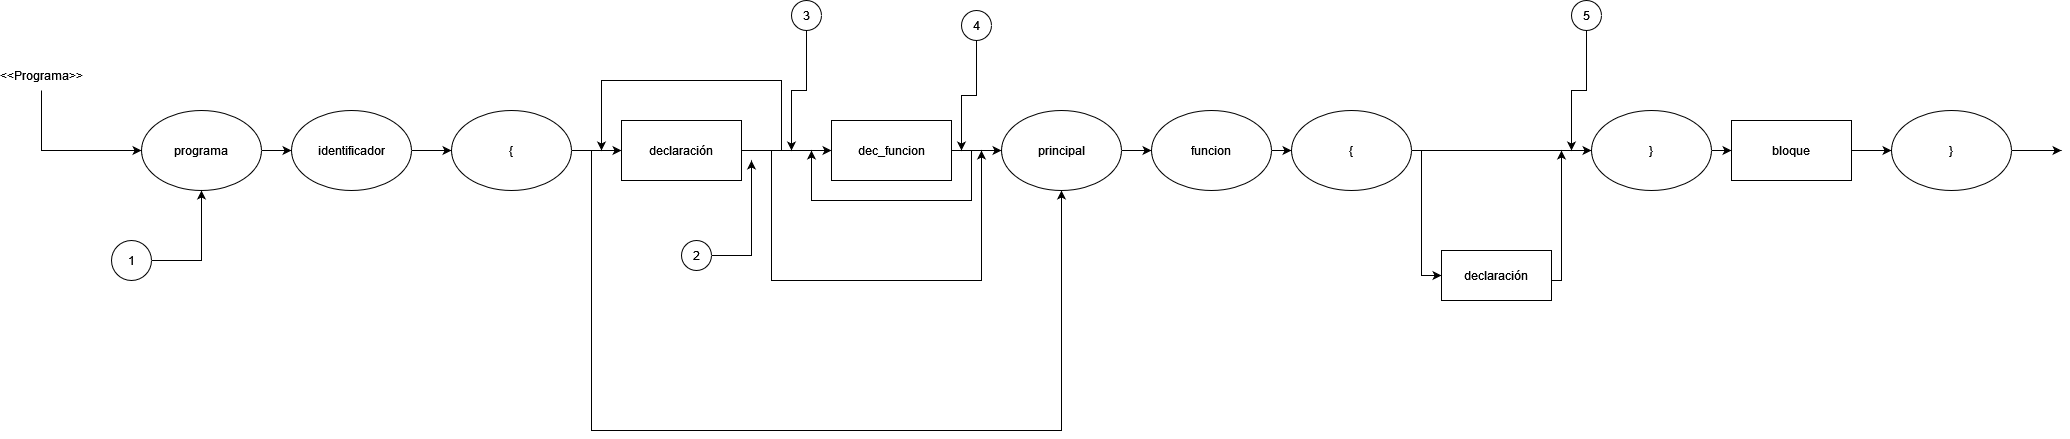
\includegraphics[width=\textwidth]{chapters/chapter3/figures/diagramas compis-Programa.drawio(1).png}
            \caption{Diagrama Programa}
            \label{fig:my_label}
    \end{figure}
    \FloatBarrier
    \item Se genera el cuádruplo de goto main y se mete el valor de contador de cuadruplos a la pila de saltos. Se actualiza la variable global del scope como global
    \item Se agrega la entrada temporal de la variable a la tabla de variables en la entrada del espacio global en el directorio de funciones.
    \item Se itera por la tabla de variables y se le asigna a cada variable una dirección virtual. Al iterar por la tabla también se actualiza el contador de recursos de las variables globales
    \item Se agrega la función a el directorio de variables
    \item Se genera la tabla de variables para el scope principal y se itera por la tabla asignando las direcciones virtuales adecuadas. Al terminar se hace pop a la pila de saltos y se actualiza el primer cuádruplo con el contador actual de cuádruplos.
    \newpage
    
    %Dec
    \begin{figure}[!htbp]
            \centering
            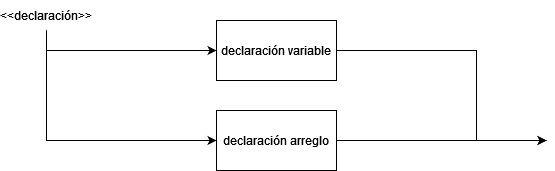
\includegraphics[width=\textwidth]{chapters/chapter3/figures/diagramas compis-declaración.drawio(1).png}
            \caption{Diagrama Declaración}
            \label{fig:my_label}
    \end{figure}
    \FloatBarrier
    % Tipo
    \begin{figure}[!htbp]
            \centering
            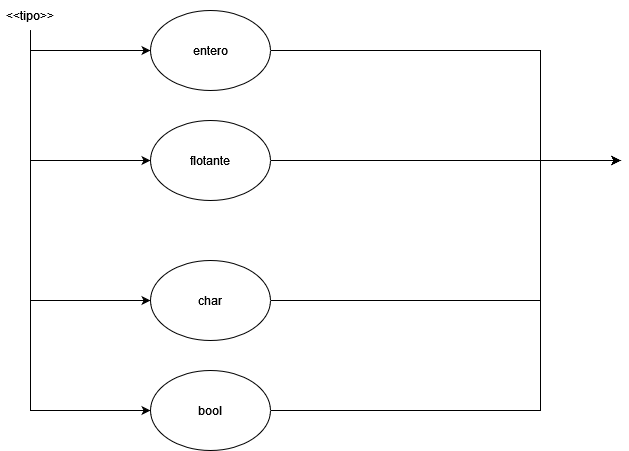
\includegraphics[width=\textwidth]{chapters/chapter3/figures/diagramas compis-tipo.drawio.png}
            \caption{Diagrama Tipo}
            \label{fig:my_label}
    \end{figure}
    \FloatBarrier
    
    %Dec de variable
    \begin{figure}[!htbp]
            \centering
            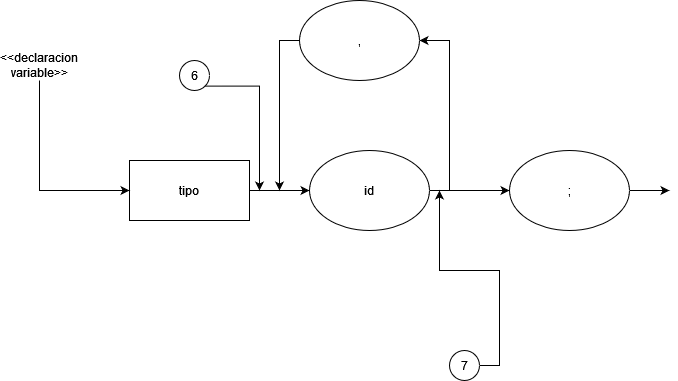
\includegraphics[width=\textwidth]{chapters/chapter3/figures/diagramas compis-declaración variable.drawio(1).png}
            \caption{Diagrama Declaración Variable}
            \label{fig:my_label}
    \end{figure}
    \FloatBarrier
    
    \item Se guarda en una variable auxiliar global el tipo de variable
    \item Se checa que el id no se repita con otros ids del scope de la declaración. Si no se repite se genera una nueva entrada de variable con el nuevo id con el tipo de variable dado por el punto 6
    
    \newpage
    %DEc de arreglo
    
    \begin{figure}[!htbp]
            \centering
            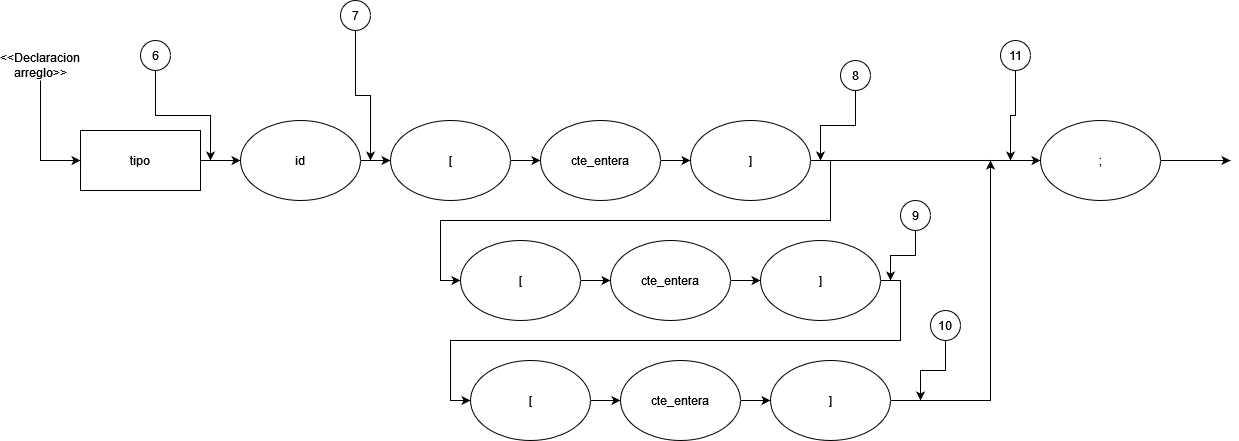
\includegraphics[width=\textwidth]{chapters/chapter3/figures/diagramas compis-declaración arreglo.drawio(1).png}
            \caption{Diagrama Declaración Arreglo}
            \label{fig:my_label}
    \end{figure}
    \FloatBarrier
    
    \item Se agrega la información de la primera dimensión a la entrada de la variable
    \item Se agrega la información de la segunda dimensión a la entrada de la variable
    \item Se agrega la información de la tercera dimensión a la entrada de la variable
    \item Se hace el cálculo de las m y el tamaño del arreglo/matriz/cubo (depende de las dimensiones leídas) y se actualiza la entrada
    
    \newpage
    % Dec Func
    
    \begin{figure}[!htbp]
            \centering
            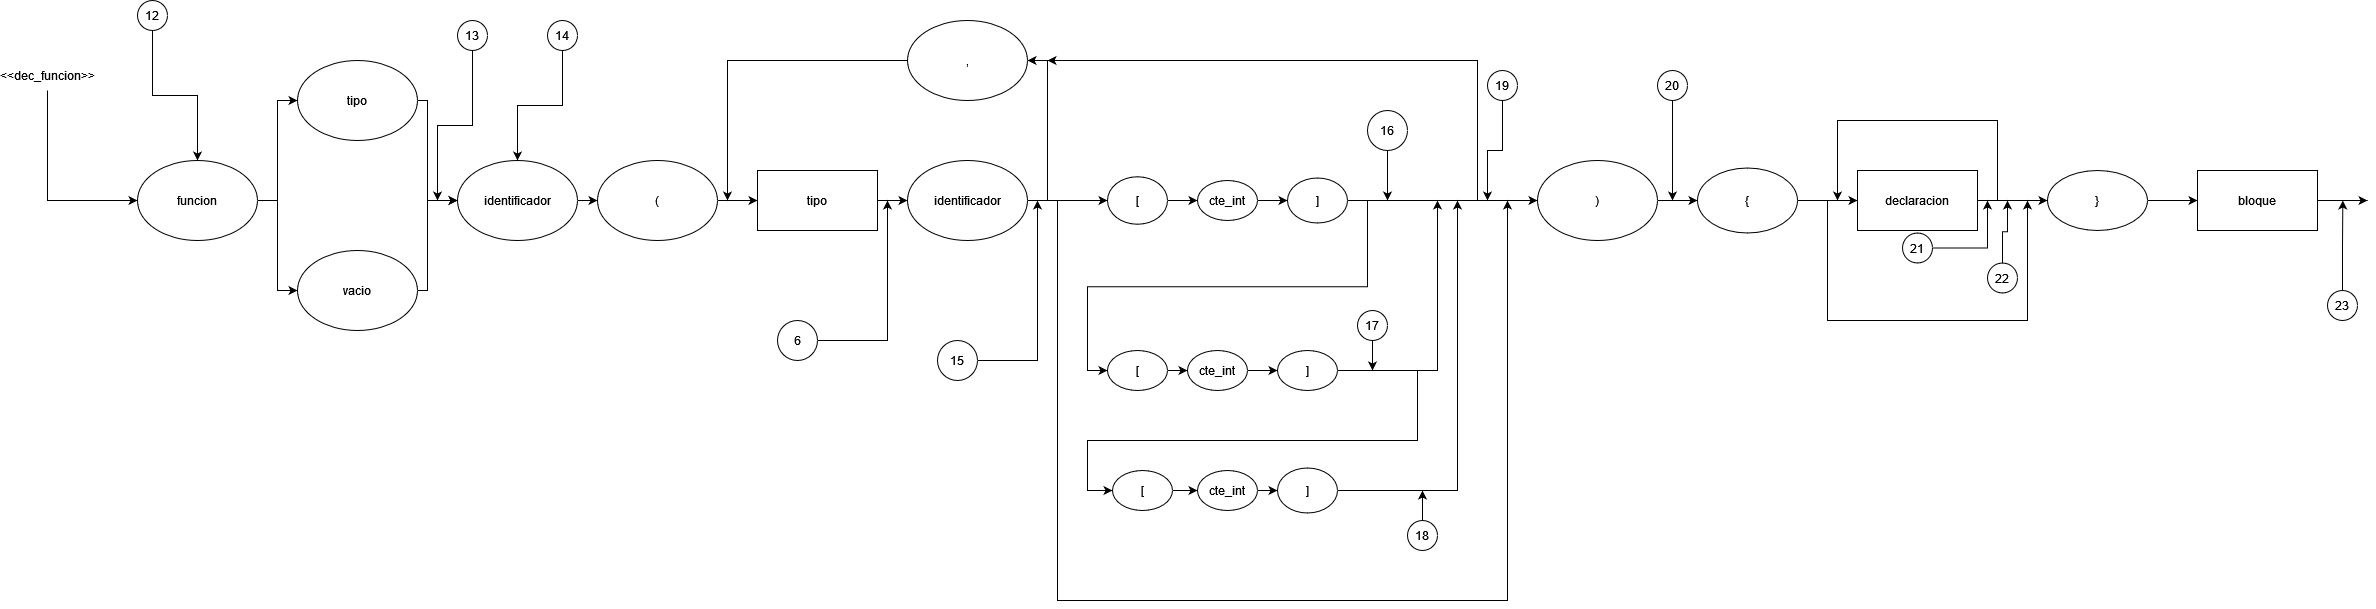
\includegraphics[width=\textwidth]{chapters/chapter3/figures/diagramas compis-dec_funcion.drawio(1).png}
            \caption{Diagrama Declaración Función}
            \label{fig:my_label}
    \end{figure}
    \FloatBarrier
    
    
    \item Se guarda en una variable auxiliar global el número del cuádruplo donde empieza la función y se genera una entrada temporal al directorio de funciones.
    \item Se guarda el tipo de función a la entrada temporal
    \item Se comprueba que el identificador no sea igual a otros identificadores, palabras clave o nombres de funciones especiales. Si no hay conflictos se agrega el nombre a la entrada temporal, si el tipo no es vacío, genera una variable global con el nombre y tipo de la función con la dirección virtual apropiada y se actualiza la variable global de scope y los contadores de recursos globales.
    \item Se checa que el id no se repita entre otros parámetros. Si no se repite se agrega el parámetro con el id y el tipo detectado a la sección de parámetros de la entrada temporal
    \item Se agrega la información de la primera dimensión a la entrada del parámetro
    \item Se agrega la información de la segunda dimensión a la entrada del parámetro
    \item Se agrega la información de la tercera dimensión a la entrada del parámetro
    \item Se hace el cálculo de las m y el tamaño del arreglo/matriz/cubo (depende de las dimensiones leídas)y se actualiza la entrada
    \item Se crean entradas a la tabla de variables locales de la funciones con la información de los parámetros
    \item Se agrega la entrada temporal de la tabla de variables a la tabla de variables local.
    \item Se itera por la tabla de variables y se le asigna a cada variable una dirección virtual.
    \item Se genera el cuádruplo de ENDFUNC y se agregan la cantidad de recursos utilizados por la función a la entrada de la función.
    
    \newpage
    
    %Bloque
    
    \begin{figure}[!htbp]
            \centering
            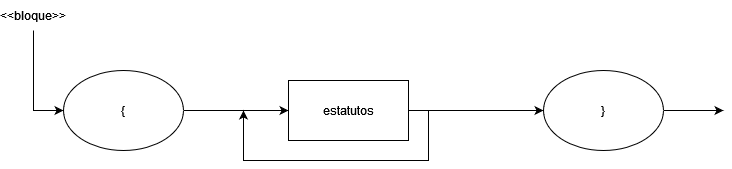
\includegraphics[width=\textwidth]{chapters/chapter3/figures/diagramas compis-bloque.drawio(1).png}
            \caption{Diagrama Bloque}
            \label{fig:my_label}
    \end{figure}
    \FloatBarrier
    
    %Estatuto
    \begin{figure}[!htbp]
            \centering
            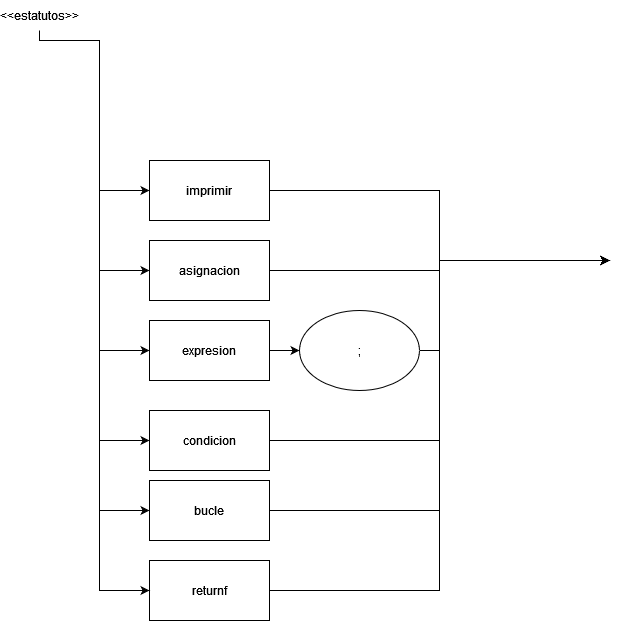
\includegraphics[width=\textwidth]{chapters/chapter3/figures/diagramas compis-estatuto.drawio(1).png}
            \caption{Diagrama Estatutos}
            \label{fig:my_label}
    \end{figure}
    \FloatBarrier
    %Return
    \begin{figure}[!htbp]
            \centering
            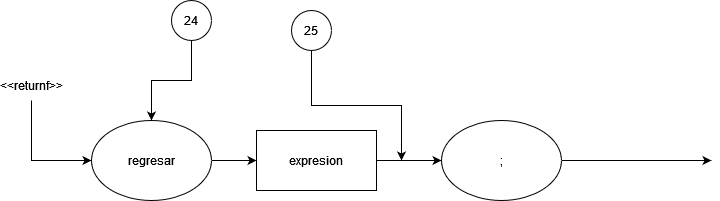
\includegraphics[width=\textwidth]{chapters/chapter3/figures/diagramas compis-returnf.drawio.png}
            \caption{Diagrama Return}
            \label{fig:my_label}
    \end{figure}
    \FloatBarrier
    \item Checar si la función que llamo a regresar no sea una función vacía. Si es vacia levantar un error
    \item Generar el cuádruplo de [RET, Dirección del resultado de la expresión, , Dirección de la variable global]
    
    \newpage
    
    %Condición
    \begin{figure}[!htbp]
            \centering
            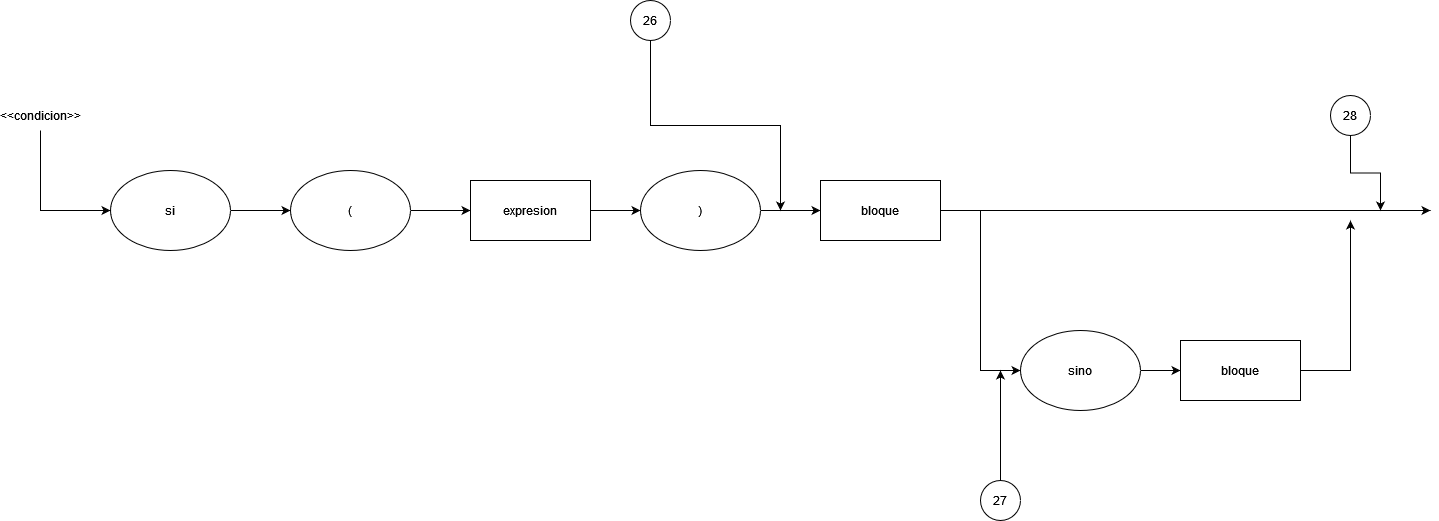
\includegraphics[width=\textwidth]{chapters/chapter3/figures/diagramas compis-condicion.drawio(1).png}
            \caption{Diagrama Condición}
            \label{fig:my_label}
    \end{figure}
    \FloatBarrier
    
    \item Se genera el cuádruplo de gotof con el resultado de la expresión y se agrega número del cuádruplo generado a la pila de saltos.
    \item Se hace pop a la pila de saltos y se genera un cuádruplo de goto y se agrega su número de cuádruplo a la pila. Se actualiza el gotof con el contador actual de cuádruplos
    \item Se hace pop a la pila de saltos y se actualiza el cuádruplo indicado por la pila con el contador actual.
    
    \newpage
    
    %Bucle
    
    \begin{figure}[!htbp]
            \centering
            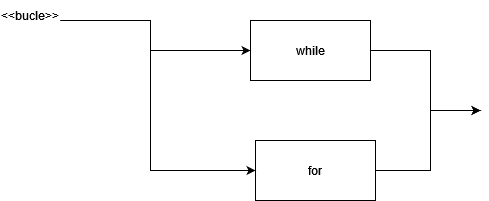
\includegraphics[width=\textwidth]{chapters/chapter3/figures/diagramas compis-bucle.drawio(1).png}
            \caption{Diagrama Bucle}
            \label{fig:my_label}
    \end{figure}
    \FloatBarrier
    
    %While
    \begin{figure}[!htbp]
            \centering
            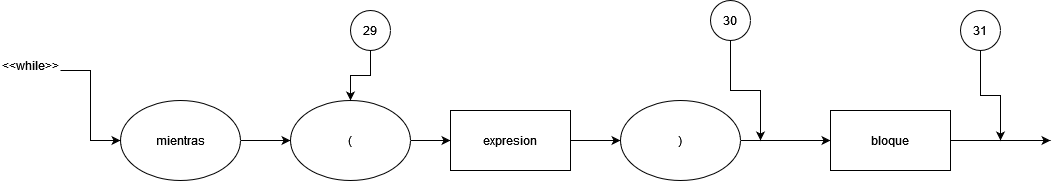
\includegraphics[width=\textwidth]{chapters/chapter3/figures/diagramas compis-while.drawio(1).png}
            \caption{Diagrama While}
            \label{fig:my_label}
    \end{figure}
    \FloatBarrier
    
    \item Se mete el contador actual de cuádruplos a la pila de operandos
    \item Se genera un cuádruplo de gotof con el resultado de la expresión y se agrega su número de contador a la pila de saltos
    \item Se le da pop dos veces a la pila de saltos y se genera un cuádruplo de goto con el segundo valor obtenido. Con el primer valor se obtiene el cuádruplo en donde esta el gotof y se actualiza con el contador actual de cuádruplos.
    
    \newpage
    %For
    \begin{figure}[!htbp]
            \centering
            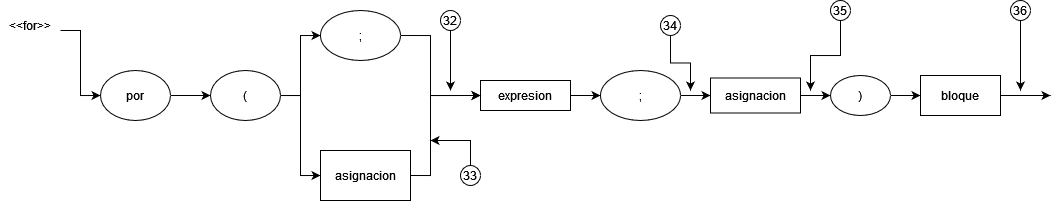
\includegraphics[width=\textwidth]{chapters/chapter3/figures/diagramas compis-for.drawio(1).png}
            \caption{Diagrama For}
            \label{fig:my_label}
    \end{figure}
    \FloatBarrier
    
    \item Se agrega el contador actual a la pila de saltos.
    \item Se checa que la asignación sea una asignación entera
    \item Se genera un gotof con la expresión y se agrega el número de cuádruplo del gotof a la pila de saltos. También se genera un cuádruplo de goto y también se agrega su número de cuádruplo a la pila de saltos.
    \item Se le hace pop a los primeros cuatro elementos de la pila de saltos. Se genera un goto al cuádruplo donde inicia la condición del for, se actualiza el cuádruplo del goto que va al bloque después de la evaluación y se vuelven a insertar los elementos sobrantes.
    \item Se le hace pop a dos elementos de la pila de operandos. Se genera un cuádruplo de goto a donde empieza la asignación de paso del for y se actualiza el cuádruplo de gotof de la condición del for.
    
    \newpage
    
    %Imprimir
    \begin{figure}[!htbp]
            \centering
            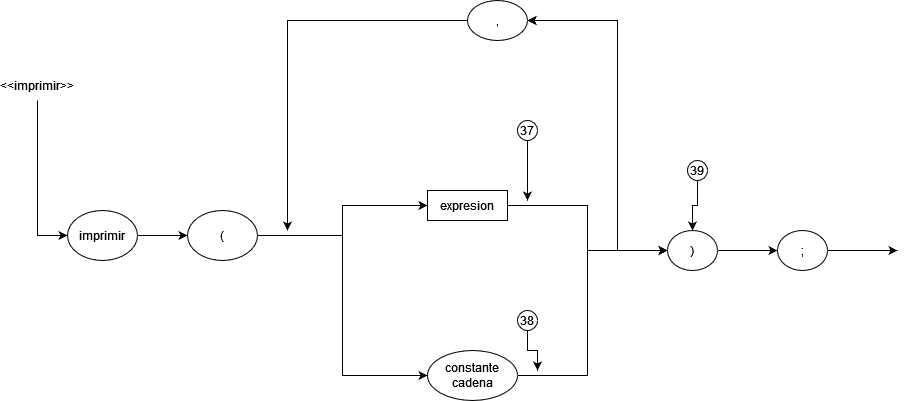
\includegraphics[width=\textwidth]{chapters/chapter3/figures/diagramas compis-imprimir.drawio(1).png}
            \caption{Diagrama Imprimir}
            \label{fig:my_label}
    \end{figure}
    \FloatBarrier
    
    \item Se le hace pop a la pila de operandos y se agrega a la fila de impresiones
    \item Se checa que la constante esta en la tabla de constantes, si no esta se agrega asignando la dirección virtual apropiada. Se agrega la dirección virtual a la pila de impresión.
    \item Se recorre la fila de impresión y se va generando un cuádruplo de imprimir con la dirección virtual en la fila
    
    \newpage
    
    %Asignación
    \begin{figure}[!htbp]
            \centering
            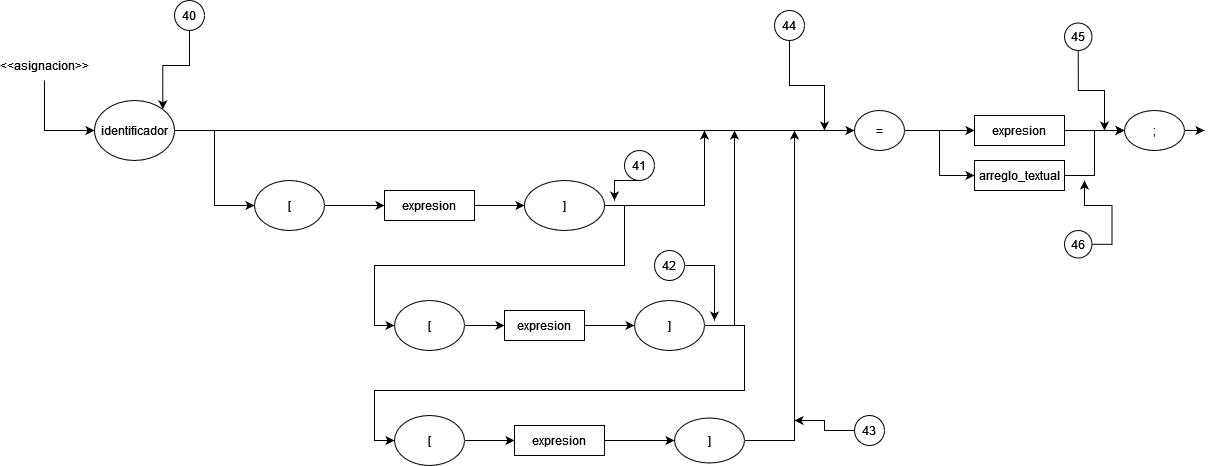
\includegraphics[width=\textwidth]{chapters/chapter3/figures/diagramas compis-asignacion.drawio(1).png}
            \caption{Diagrama Asignación}
            \label{fig:my_label}
    \end{figure}
    \FloatBarrier
    
    \item Se checa que el identificador exista en el scope local o en scope global
    \item Se hace pop a la pila de operandos y se revisa que el elemento recibido sea entero. Si es entero se agrega a la fila de subíndices.
    \item Se hace pop a la pila de operandos y se revisa que el elemento recibido sea entero. Si es entero se agrega a la fila de subíndices.
    \item Se hace pop a la pila de operandos y se revisa que el elemento recibido sea entero. Si es entero se agrega a la fila de subíndices.
    \item Se revisa si el identificador es un arreglo. Si es un arreglo se checa que la cantidad de subíndices leídos coincida con las dimensiones del arreglo, de ser así itera por los subíndices generando los cuádruplos de verificación y las sumas apropiadas para calcular la dirección virtual del arreglo accesado.
    \item Se checa contra el cubo semántico si se puede hacer la asignación. De ser posible se genera el cuádruplo de asignación apropiado.
    \item Se checa que el identificador no sea una variable simple o una llamada de arreglo. También se checa que las dimensiones del arreglo textual son iguales a las del identificador.
    
    \newpage
    
    %Expresion
    \begin{figure}[!htbp]
            \centering
            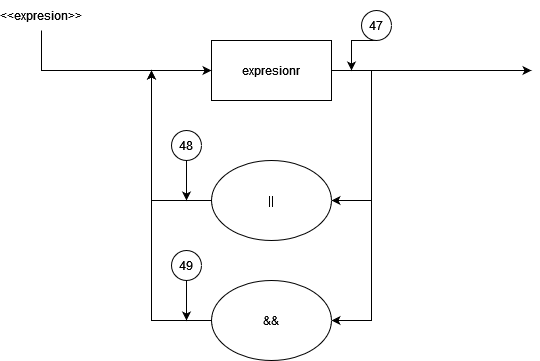
\includegraphics[width=\textwidth]{chapters/chapter3/figures/diagramas compis-expresion.drawio(1).png}
            \caption{Diagrama Expresión}
            \label{fig:my_label}
    \end{figure}
    \FloatBarrier
    
    \item Si la cima de la pila de operandos es igual a \&\& o $\parallel$, hacer pop a la pila de operandos y generar el cuádruplo de expresión correspondiente a la operador detectado.
    \item Meter $\parallel$ a la pila de operandos
    \item Meter \&\& a la pila de operandos
    
    \newpage
    
    %ExpresionR
    
    \begin{figure}[!htbp]
            \centering
            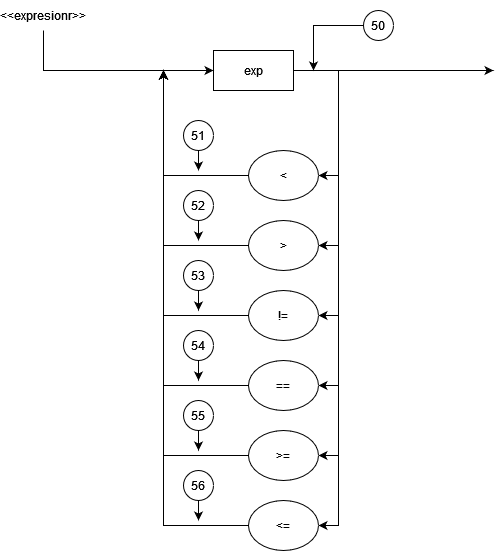
\includegraphics[width=\textwidth]{chapters/chapter3/figures/diagramas compis-expresionr.drawio.png}
            \caption{Diagrama ExpresiónR}
            \label{fig:my_label}
    \end{figure}
    \FloatBarrier
    
    \item Si la cima de la pila de operandos es igual a <, >, !=, <=, >= ó ==, hacer pop a la pila de operandos y generar el cuádruplo de expresión correspondiente a la operador detectado.
    \item Meter < a la pila de operandos
    \item Meter > a la pila de operandos
    \item Meter != a la pila de operandos
    \item Meter == a la pila de operandos
    \item Meter >= a la pila de operandos
    \item Meter <= a la pila de operandos
    \newpage
    
    %EXP
    \begin{figure}[!htbp]
            \centering
            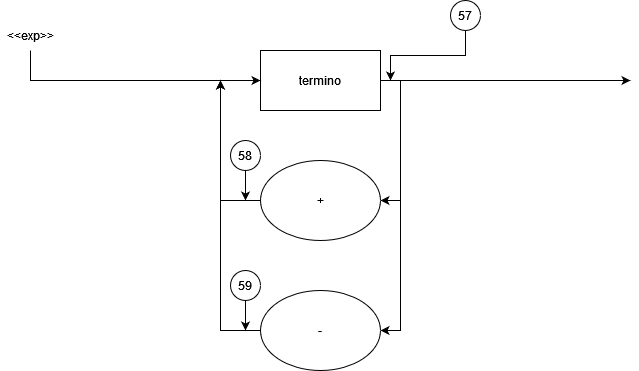
\includegraphics[width=\textwidth]{chapters/chapter3/figures/diagramas compis-exp.drawio(1).png}
            \caption{Diagrama EXP}
            \label{fig:my_label}
    \end{figure}
    \FloatBarrier
    
    \item Si la cima de la pila de operandos es igual a + ó -, hacer pop a la pila de operandos y generar el cuádruplo de expresión correspondiente a la operador detectado.
    \item Meter + a la pila de operandos
    \item Meter - a la pila de operandos
    \newpage
    
    %Termino
    \begin{figure}[!htbp]
            \centering
            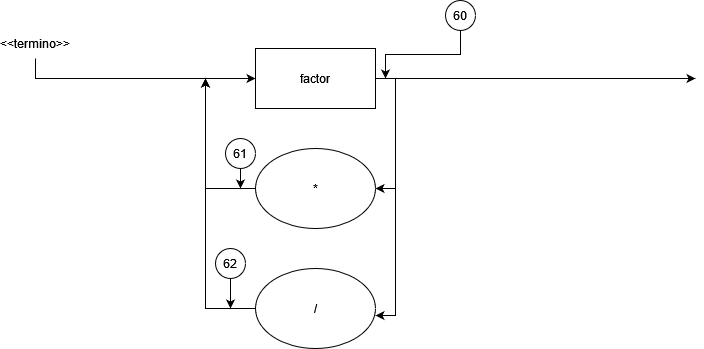
\includegraphics[width=\textwidth]{chapters/chapter3/figures/diagramas compis-termino.drawio(1).png}
            \caption{Diagrama Termino}
            \label{fig:my_label}
    \end{figure}
    \FloatBarrier
    \item Si la cima de la pila de operandos es igual a * ó /, hacer pop a la pila de operandos y generar el cuádruplo de expresión correspondiente a la operador detectado.
    \item Meter * a la pila de operandos
    \item Meter / a la pila de operandos
    \newpage
    
    %Factor
    \begin{figure}[!htbp]
            \centering
            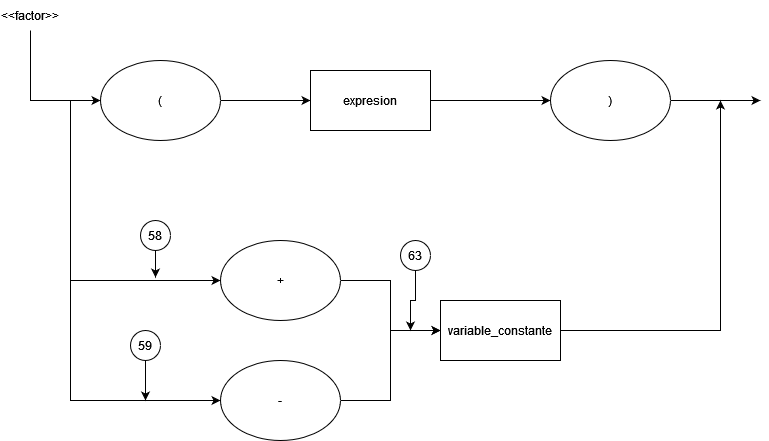
\includegraphics[width=\textwidth]{chapters/chapter3/figures/diagramas compis-factor.drawio(1).png}
            \caption{Diagrama Factor}
            \label{fig:my_label}
    \end{figure}
    \FloatBarrier
    \item Hacer pop a la pila de operador y hacer el cuádruplo de expresión unaria del operador obtenido de la pila
    
    
    \newpage
    
    %VarCte
    \begin{figure}[!htbp]
            \centering
            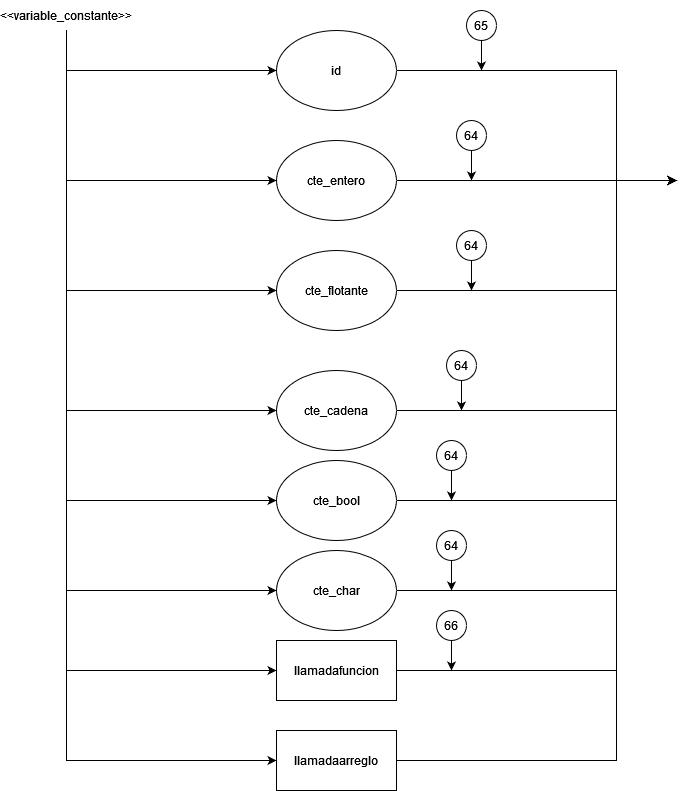
\includegraphics[width=\textwidth]{chapters/chapter3/figures/diagramas compis-variable_constante.drawio(1).png}
            \caption{Diagrama Variable\_Constante}
            \label{fig:my_label}
    \end{figure}
    \FloatBarrier
    \item Checar si la constante existe en la tabla de constantes, si no existe se agrega a la tabla de constantes con la dirección virtual apropiada. Agregar la dirección virtual de la constante a la pila de operandos
    \item Checar si el id existe en el scope local o global. Si existe agregar su dirección virtual a la pila de operandos.
    \item Checa si la llamada a función es de retorno. Si es de retorno crear una variable temporal con el valor actual de la variable global de la función y agregar el temporal a la pila de operandos
    
    
    \newpage
    
    %Llamada Arreglo
    \begin{figure}[!htbp]
            \centering
            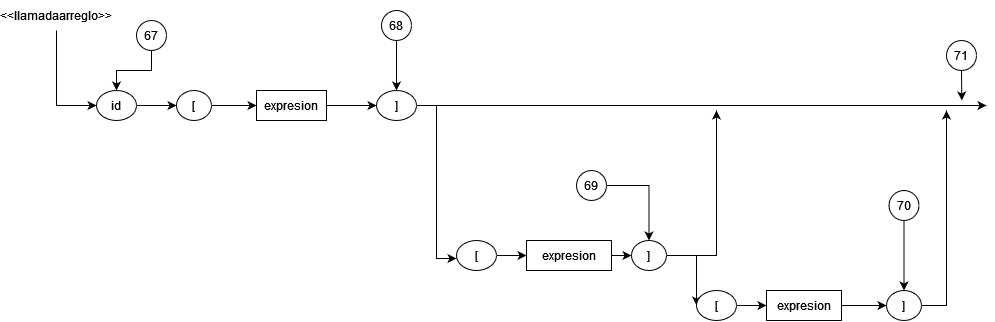
\includegraphics[width=\textwidth]{chapters/chapter3/figures/diagramas compis-llamadaarreglo.drawio.png}
            \caption{Diagrama Llamada Arreglo}
            \label{fig:my_label}
    \end{figure}
    \FloatBarrier
    \item Se revisa si el identificador es un arreglo. 
    \item Se hace pop a la pila de operandos y se revisa que el elemento recibido sea entero. Si es entero se agrega a la fila de subíndices.
    \item Se hace pop a la pila de operandos y se revisa que el elemento recibido sea entero. Si es entero se agrega a la fila de subíndices.
    \item Se hace pop a la pila de operandos y se revisa que el elemento recibido sea entero. Si es entero se agrega a la fila de subíndices.
    \item Se checa que la cantidad de subíndices leídos coincida con las dimensiones del arreglo, de ser así itera por los subíndices generando los cuádruplos de verificación y las sumas apropiadas para calcular la dirección virtual del arreglo accesado.
    
    \newpage
    % Llamada función
    \begin{figure}[!htbp]
            \centering
            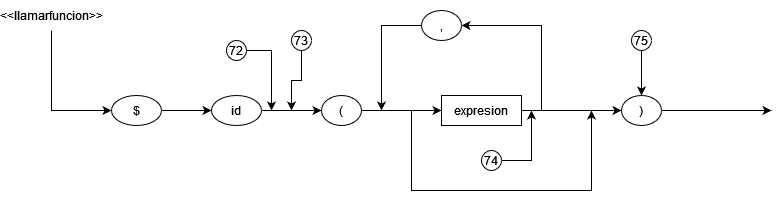
\includegraphics[width=\textwidth]{chapters/chapter3/figures/diagramas compis-llamarfuncion.drawio.png}
            \caption{Diagrama Llamada Función}
            \label{fig:my_label}
    \end{figure}
    \FloatBarrier
    
    \item Checar si es una función especial. Si es función especial, crear una variable global con el nombre y tipo de la función y la dirección de memoria apropiada.
    \item Obtener la información de los parámetros del directorio de funciones y generar el cuádruplo de era.
    \item Hacer pop a la pila de operandos y meter el elemento obtenido a una fila de parámetros.
    \item Comparar si los elementos de la fila de parámetros coinciden con los parámetros de la función. Si los elementos coinciden generar los cuádruplos de parameter apropiados para cada elemento de la fila.
    
    \newpage
    % Arreglo Textual
    \begin{figure}[!htbp]
            \centering
            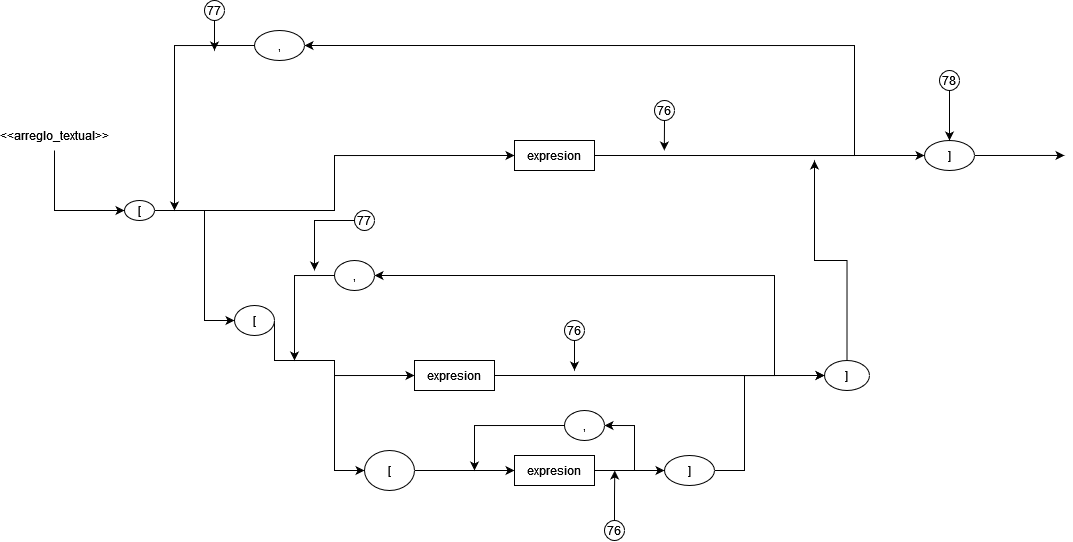
\includegraphics[width=\textwidth]{chapters/chapter3/figures/diagramas compis-arreglo_textual.drawio.png}
            \caption{Diagrama Arreglo\_Textual}
            \label{fig:my_label}
    \end{figure}
    \FloatBarrier
    
    \item Se checa el tipo de la expresión realizada y se mete a un stack auxiliar de tipos y se checa la congruencia de tipo con los demás leídos (si hay).
    \item Se checa la congruencia de la dimensión del elemento leído, si las dimensiones son diferentes se levanta un error. Igual se guarda el tamaño de las dimensiones leídas.
    \item Se calcula el tamaño del arreglo/cubo/matriz  
    
    

\end{enumerate}
\newpage
\FloatBarrier
%---------------------------------------------------------------------------------------
\section{Descripción de Administración de Memoria usado en la compilación}

Para la administración de memoria duarante compilación se usaron princiaplemente los siguientes elementos:

\begin{enumerate}

    \item Directorio de Funciones
    \item Vector de Cuadruplos y su contador
    \item Tabla de Constantes y su espejo
    \item Cubo Semantico
    \item Contadores Globales de Variables Globales y temporales
    \item Máximos de Variables y las direcciones de memoria
    \item Vector de relación linea código fuente a cuadruplo
    \item Variables auxiliares para el manejo de arreglos
    \item Pila de operadores, Pila de operandos y Pila de tipos
    \item Diccionario de funciones especiales
    
\end{enumerate}

Cada uno de estos se va a explicar con más detalle en las siguientes subsecciones.

\subsubsection{Directorio de Funciones y el Directorio de Funciones Especiales}

Para implementar el directorio de funciones se requería una estructura de datos que fuera de acceso rápido y que pudiera contener muchos tipos de variables e información dentro de ella. Afortunadamente en el lenguaje de Python no hay mucha restricción sobre el tipo de datos que se guardan en sus diferentes estructuras. Dado lo que se necesitaba que fuera el directorio de funciones se decidió utilizar la estructura de Diccionario de Python. Este nos permitiría guardar cualquier información necesaria con una llave única, además permite guardar cualquier otra estructura de datos dentro de cada entrada de un diccionario permitiendo una gran flexibilidad de la información que se puede guardar. También los diccionarios son de las estructuras son de rápido acceso para consultas.


\begin{table}[htbp]
    \centering
    %\tiny
    \begin{tabular}{|c|c|c|c|c|c|c|}
        nombre & tipo & address & params & varres & tmpres & vartab \\ \hline
        
         global & vacio & - & - & 1,0,1,1 & - & \tiny Dict de python de var  \\
         pop & vacio & -  & \tiny Dict de python de params & 1,0,3,1 & 14, 1, 2, 7, 0 & \tiny Dict de python de var \\
         principal & vacio & - & \tiny Dict de python de params & 1,0,1,1 & 14, 0, 0, 7, 0 & \tiny Dict de python de var  \\
    \end{tabular}
    \caption{Representación Lógica del directorio de funciones}
    \label{tab:my_label}
\end{table}
\FloatBarrier
Cada entrada de la tabla tiene cinco elementos importantes. El primero es el tipo de la función, este ayuda a identificar si la función tiene retorno o es vacía. La segunda es address. Esta es la dirección virtual de la función si es función de retorno. La tercera es params que es un diccionario de Python que tiene la información del tipo e información de arreglos si el parámetro es un arreglo. El tercero y cuarto elemento son una serie de contadores que representan los recursos locales y temporales respectivamente que tiene una función. El quinto elemento es la tabla de variables que contiene la información de las variables locales de la función.

En el caso de la entrada global, es la única entrada del directorio que no cuenta con información de variables temporales.


Para facilitar la integración de las funciones especiales en compilación también se usó una estructura muy similar al directorio de funciones. De esta manera se pueden usar muchos de los métodos para recorrer el directorio de funciones en el directorio de funciones especiales. Realmente la única diferencia que existe entre los dos es que el directorio de funciones especiales no cuenta con un contador de variables temporales ni una tabla de variables, ya que para ejecutar estas funciones en la máquina virtual solo se necesita saber la información de los parámetros.


\begin{table}[htbp]
    \centering
    %\tiny
    \begin{tabular}{|c|c|c|c|c|c|c|}
        nombre & tipo & address & params & varres \\ \hline
        
         normal & flotante & 1006 & \tiny Dict de python de params  & 2,0,0,0  \\
         modulo & flotante & 1007  & \tiny Dict de python de params & 2,0,0,0  \\
    \end{tabular}
    \caption{Representación Lógica del directorio de funciones especiales}
    \label{tab:my_label}
\end{table}
\FloatBarrier

\FloatBarrier
\subsubsection{Vector de Cuadruplos y su contador}

Para representar los cuádruplos se utilizaron la estructura de tuplas de Python. Pero un programa no cuenta con un solo cuádruplo sino una serie de múltiples cuádruplos ordenados que indican las instrucciones a ejecutar a la máquina virtual. Para lograr esto se creó una lista de tuplas, a la cual se le va agregando como en una fila cada cuádruplo generado. Para tener un mejor control sobre la cantidad de cuádruplos generados también se mantuvo una variable auxiliar global contadora de cuádruplos.

\begin{figure}[htbp]
    \centering
    \begin{lstlisting}[language=Python]
        ('GOTO','','',20)
    \end{lstlisting}
    \caption{Ejemplo de una tupla de Cuádruplo}
    \label{fig:my_label}
\end{figure}

\begin{figure}[htbp]
    \centering
    \begin{lstlisting}[language=Python]
        cuadruplos.append(('GOTOF',res,''))
        global sclines
        sclines.append(p.lineno(1))
        psaltos.append(cuadcount)
        cuadcount += 1
    \end{lstlisting}
    \caption{Ejemplo de generación de un cuádruplo}
    \label{fig:my_label}
\end{figure}
\FloatBarrier

\subsubsection{Tabla de Constantes y su espejo}

Como el directorio de funciones, la tabla de constantes también va a ser una estructura que va a ser consultada muy frecuente mente. Como se había mencionado previamente, el diccionario de Python también es una buena solución para poder guardar y acceder con mucha facilidad información de manera frecuente. Por ello se optó por usar también el diccionario de Python para representar la tabla de constantes.


\begin{table}[htbp]
    \centering
    \begin{tabular}{c|c}
         Constante & Dirección \\ \hline
         25000 & 2 \\
         25001 & 1 \\
         310000 & "Hola" \\
    \end{tabular}
    \caption{Representación Lógica de la tabla de constantes}
    \label{tab:my_label}
\end{table}
\FloatBarrier

\begin{figure}[htbp]
    \centering
    \begin{lstlisting}[language=Python]
        {                                         
            "2": 25000,                            
            "1": 25001,                            
            "3": 25002,                            
            "1001": 25003,                         
            "1003": 25004,                         
            "3000": 25005,                         
            "0": 25006,                            
            "5": 25007,                            
            "\"Factorial de n \\n\"": 31000,       
            "10": 25008,                           
            "\"Factorial Secuencial : \"": 31001,  
            "\"------\\n hola aka =\"": 31002      
        }                                           
    \end{lstlisting}
    \caption{Ejemplo de el diccionario de constantes}
    \label{fig:my_label}
\end{figure}
\FloatBarrier

Como Python no es un lenguaje fuertemente tipado, para generar las llaves del diccionario se transforma a string la constante para poderla encontrar fácilmente. También para reducir el tiempo de ejecución a la hora de crear el archivo obj, se mantiene una copia de la tabla de constantes con el formato correcto para la máquina virtual.
\begin{figure}[htbp]
    \centering
    \begin{lstlisting}[language=Python]
        {
            "25000": 3,
            "25001": 1,
            "25002": 9,
            "25003": 9003,
            "25004": 14001,
            "25005": 9006,
            "25006": 10,
            "25007": 30,
            "25008": 2,
            "25009": 1000000,
            "25010": 20,
            "30000": true,
            "31000": "\"Hola Mundo\"",
            "25011": 0,
            "31002": "\"Iteracion por la matriz\"",
            "31003": "\"Iteracion por el cubo\"",
            "31004": "\"\\t--Dim2\"",
            "31005": "\"\\t\\t---Dim 3\"",
            "31006": "\"Probando arreglos textuales\"",
            "29000": "'a'",
            "25012": 4,
            "25013": 5,
            "25014": 6,
            "29001": "'b'",
            "29002": "'c'",
            "30001": false,
            "25015": 127
        }
    \end{lstlisting}
    \caption{Ejemplo de el diccionario de constantes para la máquina virtual}
    \label{fig:my_label}
\end{figure}

\FloatBarrier

\subsection{Tabla de variables}

Para la tabla de variables también se necesitó una estructura de datos que se rápida de acceder y modificar. Como se mencionó con el directorio de funciones, el diccionario de Python resulto ser una estructura de datos que se adaptaba muy bien a solucionar este problema. Por ello también se utilizó un diccionario de Python para representar la tabla de variables.


\begin{table}[htbp]
    \centering
    \begin{tabular}{c|c|c|c|c}
        nombre & tipo & dirección & dims & dimlen   \\
        a & entero & 1000 & - & - \\
        b & entero & 1001 & 2 & [3,4], [4,0] \\
    \end{tabular}
    \caption{Representación Lógica de la tabla de variables}
    \label{tab:my_label}
\end{table}
\FloatBarrier
El diccionario de la tabla de variables constaba de que cada llave fuera el nombre de la variable y que dentro de esa llave se guardara otro diccionario con la información de la variable. Este diccionario tiene lo que es el tipo de la variable, su dirección de memoria, y si es un arreglo, las dimensiones del arreglo y la información para calcular la indexación.

\subsubsection{Cubo Semántico}

Para el cubo semántico se decidió ir por una estructura que pudiera ser accesada rápidamente y que pudiera dar el resultado de una operación con llaves sencillas. Ya que se trabajó en el lenguaje de Python, se aprovechó de la estructura nativa de diccionarios. Estos pueden ser accesados rápidamente y se le pueden asignar llaves a cada entrada. Para hacer el código legible se decidió estructurar el cubo como un diccionario de diccionarios. De esta manera la llamada al cubo semántico sería accesando al cubo con la primera llave siendo el operador, y las otras dos llaves siendo el operando izquierdo y el operando derecho.


\begin{table}
    \centering
    \caption{Tabla representando el cubo semántico}
    \small
    \begin{tabular}{||c c || c c c c c c c c c c c c c||} 
         
         OpIzq & OpDer & $=$ & $\parallel$ & \&\& & \textless & \textgreater & \textless $=$ & \textgreater $=$ & !$=$ & $==$ & $+$ & $-$ & * & \textbackslash \\ [0.5ex] 
         \hline\hline
         ent & ent & ent & bool & bool & bool & bool & bool & bool & bool & bool & ent & ent & ent & ent \\ 
         \hline
         ent & flot & ent & bool & bool & bool & bool & bool & bool & bool & bool & flot & flot & flot & flot \\ 
         \hline
         ent & char & ent & bool & bool & bool & bool & bool & bool & bool & bool & ent & ent & ent & ent \\ 
         \hline
         ent & bool & ent & bool & bool & bool & bool & bool & bool & bool & bool & ent & ent & ent & ent \\ 
         \hline
         ent & cadena & err & err & err & err & err & err & err & err & err & err & err & err & err \\ 
         \hline
         flot & ent & flot & bool & bool & bool & bool & bool & bool & bool & bool & flot & flot & flot & flot \\ 
         \hline
         flot & flot & flot & bool & bool & bool & bool & bool & bool & bool & bool & flot & flot & flot & flot \\ 
         \hline
         flot & char & flot & bool & bool & bool & bool & bool & bool & bool & bool & flot & flot & flot & flot \\ 
         \hline
         flot & bool & flot & bool & bool & bool & bool & bool & bool & bool & bool & flot & flot & flot & flot \\ 
         \hline
         flot & cadena & err & err & err & err & err & err & err & err & err & err & err & err & err \\ 
         \hline
         char & ent & char & bool & bool & bool & bool & bool & bool & bool & bool & ent & ent & ent & ent \\ 
         \hline
         char & flot & char & bool & bool & bool & bool & bool & bool & bool & bool & flot & flot & flot & flot \\ 
         \hline
         char & char & char & bool & bool & bool & bool & bool & bool & bool & bool & ent & ent & ent & ent \\ 
         \hline
         char & bool & char & bool & bool & bool & bool & bool & bool & bool & bool & ent & ent & ent & ent \\ 
         \hline
         char & cadena & err & err & err & err & err & err & err & err & err & err & err & err & err \\ 
         \hline
         bool & ent & bool & bool & bool & bool & bool & bool & bool & bool & bool & ent & ent & ent & ent \\ 
         \hline
         bool & flot & bool & bool & bool & bool & bool & bool & bool & bool & bool & flot & flot & flot & flot \\ 
         \hline
         bool & char & bool & bool & bool & bool & bool & bool & bool & bool & bool & ent & ent & ent & ent \\ 
         \hline
         bool & bool & bool & bool & bool & bool & bool & bool & bool & bool & bool & ent & ent & ent & ent \\ 
         \hline
         bool & cadena & err & err & err & err & err & err & err & err & err & err & err & err & err \\ 
         \hline
         cadena & ent & err & err & err & err & err & err & err & err & err & err & err & err & err \\ 
         \hline
         cadena & flot & err & err & err & err & err & err & err & err & err & err & err & err & err \\ 
         \hline
         cadena & char & err & err & err & err & err & err & err & err & err & err & err & err & err \\ 
         \hline
         cadena & bool & err & err & err & err & err & err & err & err & err & err & err & err & err \\ 
         \hline
         cadena & err & err & err & err & err & err & err & err & err & err & err & err & err & err \\ 
        
         
        
        \end{tabular}
        \begin{itemize}
            \item ent : Entero
            \item flot : Flotante
            \item err : Error
        \end{itemize}
    
\end{table}
\FloatBarrier

\begin{figure}[htbp]
    \centering
    \begin{lstlisting}[language=Python]
        rettype = ptipo.pop()
        if (cubosem['='][functipo][rettype] != 'error'):
            dprint('Cubo dice: ',cubosem['='][functipo][rettype])
            retop = pilaoperand.pop()
            ......
    \end{lstlisting}
    \caption{Ejemplo del uso de el Cubo Semántico}
    \label{fig:my_label}
\end{figure}
\FloatBarrier
\begin{figure}[htbp]
    \centering
    \begin{lstlisting}[language=Python]
        cubosem = {
        '=':{
            'entero':{
                        'entero':'entero',
                        'flotante': 'entero',
                        'char':'entero',
                        'bool': 'entero',
                        'cadena':'error'
                    },
            'flotante':{
                        'entero':'flotante',
                        'flotante': 'flotante',
                        'char':'flotante',
                        'bool': 'flotante',
                        'cadena':'error'
                    },
            'char':{
                        'entero':'char',
                        'flotante': 'char',
                        'char':'char',
                        'bool': 'char',
                        'cadena':'error'
                    },
            'bool':{
                        'entero':'bool',
                        'flotante': 'bool',
                        'char':'bool',
                        'bool': 'bool',
                        'cadena':'error'
                    },
            'cadena':{
                        'entero':'error',
                        'flotante': 'error',
                        'char':'error',
                        'bool': 'error',
                        'cadena':'err'
                    },

            },
        .....
    \end{lstlisting}
    \caption{Muestra de la primera entrada del cubo semántico}
    \label{fig:my_label}
\end{figure}
\FloatBarrier




\subsubsection{Contadores Globales de Variables Globales y temporales, Máximos de Variables y las Direcciones de Memoria}

Para mantener un registro del uso de recursos dentro del programa durante el proceso de compilación se crearon variables globales que funcionaban como contadores sobre cada tipo de variable. Cada vez que se generaba una nueva variable se aumentaba el contador y se verificaba que no se pasara de los máximos del tipo permitidos. Estos contadores se dejaron como variables globales porque había múltiples acciones semánticas que requerían consultar o actualizar sus valores. Para mantener legibilidad y por simplicidad se optó por dejarlo como variables globales.

\begin{table}[htbp]
    \centering
    \begin{tabular}{c|c|c|c|c}
        \multicolumn{5}{c}{Globales} \\\hline
         Enteros & Flotantes & Caracteres & Booleanos & Apuntadores  \\
          1 & 2 & 0 & 3 & 0 \\\hline\hline
          
          \multicolumn{5}{c}{Temporales} \\
         Enteros & Flotantes & Caracteres & Booleanos & Apuntadores  \\
          8 & 2 & 0 & 6 & 0 
    \end{tabular}
    \caption{Representación Lógica de los Contadores Globales}
    \label{tab:my_label}
\end{table}
\FloatBarrier
Similar que con los contadores globales también se dejó los máximos de variables y de direcciones de memoria como variables globales para mantener legibilidad y simplicidad en el código. Como muchas de las acciones semánticas también interactuar con ellas se mantienen globales.

\subsubsection{Vector de relación línea código fuente a cuádruplo}

Para desarrollar mensajes de error más detallados en la máquina virtual, se necesitaba saber en qué línea de código se causó el error. Para resolver este problema se creó una lista que aprovecha el rastreador de tokens del lexer de \emph{ply} para guardar el número de la línea del código fuente en relación con un cuádruplo. Esta lista va creciendo a la par que la lista de cuádruplos y es pasada como información a la máquina virtual para que pueda usarla en sus mensajes de error.


\begin{figure}[htbp]
    \centering
    \begin{lstlisting}
    // La lista de cuadruplos
        Cuadruplos = [('GOTO','MAIN','',''), 
        ("*", 25006, 25007, 17000), 
        ("/", 17000, 25007, 17001), 
        ("*", 17001, 25008, 17002), 
        ......]
    // Lista de la linea de codigo fuente que la creo
        sclines = [1, 9, 9, 9, 9, ......]
    \end{lstlisting}
    \caption{Ejemplo de como se ve la relación de cuádruplos contra líneas de código fuente}
    \label{fig:my_label}
\end{figure}
\FloatBarrier
\subsubsection{Variables auxiliares para el manejo de arreglos}

Para el cálculo de la información de la indexación de arreglos se optó por dejar las variables como variables globales. Como no son muchas las variables para el cálculo de la fórmula de indexación, ya que este lenguaje se limita hasta cubos nada más, no se vio necesario crear una estructura extra para manejar su información. De igual manera, como son múltiples acciones semánticas que utilizan estas variables por conveniencia se dejaron como variables globales.


\begin{table}[htbp]
    \centering
    \begin{tabular}{|c|c|}
       R  &  1\\
      at1 & 2 \\
      at2 & 3 \\
      at3 & 0 \\
    \end{tabular}
    \caption{Representación Lógica de las Varables Auxiliares de arreglos}
    \label{tab:my_label}
\end{table}

\FloatBarrier
\subsubsection{Pila de operadores, Pila de operandos y Pila de tipos}

Para el manejo de la lógica de expresiones como visto en clase se necesitaba utilizar una estructura stack para el manejo de las acciones semánticas. Python no cuenta con una estructura stack, pero cuenta con métodos que simulan a un stack en su estructura de lista. Por ello se manejó la Pila de Operadores, Pila de Operandos y la Pila de tipos como listas las cuales solo se podían interactuar con usando los métodos de \emph{pop} y \emph{append} que tienen las listas.

\begin{table}[htbp]
    \centering
    \begin{tabular}{c|c c c c}
         \hline
        Pila de Operadores & + & * & & ....   \\\hline \hline
        Pila de Operandos &  A & 1000 & x\_inicial & ....\\\hline \hline
        Pila de Tipos & entero & entero & entero & .... \\\hline \hline
    \end{tabular}
    \caption{Representación Lógica de las Pilas}
    \label{tab:my_label}
\end{table}


%\part{Descripción de la máquina virtual}
\chapter{Descripción de la máquina virtual}

En esta parte se describe con más detalle lo que se utilizo para la máquina virtual y su manejo de memoria

\section{Equipo de cómputo, lenguaje y utilerías especiales usadas}

Una PC con Windows 10, se utilizó el lenguaje de programación Python 3.10 con apoyo de las librerías de \emph{PLY, Numpy, re, json, SciPy y Matplotlib}.

La máquina virtual utiliza las librerías de emph{JSON, SciPy, NumPy y Matplotlib}. Utiliza la librería de \emph{JSON} para leer el archivo generado por el compilador y con toda la información del archivo va ejecutando el código intermedio generado por el compilador. Cuando la máquina lee una función especial utiliza las librerías de \emph{SciPy, NumPy y Matplotlib} para ejecutar dichas funciones.


\section{Descripción del proceso de Administración de Memoria en ejecución}
Para lograr ejecutar de manera correcta el código compilado es importante poder representar y manejar el espacio de memoria en la máquina virtual, de manera en la que se pueda convertir las direcciones virtuales asignadas por el compilador a espacios de memoria en la máquina.

\subsection{La Clase Memoria}

Para manejar la memoria en la máquina virtual se desarrollo la clase Memory, la cual representa un conjunto de espacios de memoria para enteros, flotantes, caracteres, booleanos y apuntadores como cinco listas. Esta clase recibe un número representando la cantidad de espacios para cada tipo de variable en su constructor y se genera una lista con el tamaño apropiado.

%Diagrama de clase de Memory
\begin{figure}[htbp]
    \centering
    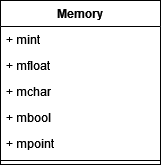
\includegraphics[scale=0.6]{chapters/chapter4/figures/Class_Memeory.png}
    \caption{Diagrama de Clase de Memory}
    \label{fig:my_label}
\end{figure}
\FloatBarrier
De esta manera se puede mapear la memoria de la máquina virtual, las listas que contienen la información, a las direcciones virtuales del compilador realizando la siguiente formula.
$$Espacio\_en\_el\_arreglo = Dir\_Virtual - Dir\_Virtual\_Base\_del\_tipo$$
Con esta formula se puede sacar la posición en el arreglo se encuentra el valor de la variable.


\subsection{Manejo de memoria global, local y temporal}

Ahora para representar el espacio de memoria en la máquina virtual se necesita primero plantear el como se debe de manejar los scopes de las variables. Para manejar las variables globales basta con crear una instancia de Memory para representarlas, pero se empieza a complicar la situación cuando se intenta representar el scope de la función principal o de cualquier otra función. Esto se debe a que Memory solo cuenta con un conjunto de arreglos, pero estos espacios de memoria cuentan no solo con variables locales sino que también con variables temporales. Para lidiar con este problema el espacio de memoria de una función se representa por un vector con dos instancias de Memory. La primera representando las variables locales y la segunda representando las variables temporales.
% imagen representando esto

\begin{figure}
    \centering
    \begin{lstlisting}[language=Python]
        globalMem = Memory(1,6,0,3)
        # El primero representa el local y el segundo el temporal
        principalMem = [Memory(1,6,0,3), Memory(7,6,0,8)] 
    \end{lstlisting}
    \caption{Representación en código de las memorias}
    \label{fig:my_label}
\end{figure}
\FloatBarrier

Con este vector ahora ya se puede manejar todos los posibles scopes de la memoria.


\subsection{El stack de memorias}

Habiendo resuelto el problema de las variables temporales y locales, surge un nuevo problema. ¿Cómo se sabe en qué memoria se está trabajando actualmente? Para resolver esto se implemento una pila, la cual maneja el contexto actual con el que se esta trabajando. La idea de usar una pila viene a la naturaleza del uso de espacios de memoria cuando se llama a una función. 
Lógicamente si seguimos el algoritmo que generan los cuádruplos, la máquina virtual va a parar la ejecución del código actual y va a saltar a realizar el código de la función. Después de acabar la función la máquina debe de regresar a donde estaba y continuar el código. Esto se podría resolver con una variable auxiliar, pero surge un problema si se utiliza una variable auxiliar cuando una función llama a otra función. 
% ejemplo con listings

\begin{figure}[htbp]
    \centering
    \begin{lstlisting}[language = Python]
        # Se llama funcion 1
        auxMem = principalMem
        .........
        # Se llama funcion 2
        auxMem = funcMem
        # Ya se perido la memoria de principal 
    \end{lstlisting}
    \caption{Representación de el uso de una variable auxiliar}
    \label{fig:my_label}
\end{figure}
\FloatBarrier
Si solo se usa una variable auxiliar la nueva función va a causar que la memoria de la función que se anda ejecutando sobre escriba a la memoria que la llamo. Pero este problema se puede resolver con una pila. Si una función llama a otra función en su ejecución lo que se puede hacer es ir guardando las memorias en la pila y cuando se dejen de utilizar se remueven del tope de la pila y se continúa utilizando el siguiente elemento en la pila. De esta manera se resuelve el problema de cuando una función llama a otra función.
\begin{figure}[htbp]
    \centering
    \begin{lstlisting}[language = Python]
        # Se llama funcion 1
        auxMem.append(principalMem)
        .........
        # Se llama funcion 2
        auxMem.append(funcMem)
        # Ahora solo se tiene que hacer pop al stack para obtener el contexto pasado
    \end{lstlisting}
    \caption{Representación de el uso de una pila para el manejo de memoria}
    \label{fig:my_label}
\end{figure}
\FloatBarrier
Esta solución no solo aplica para las funciones que son dependientes a otras, sino que también soluciona el problema de el manejo de memorias en funciones recursivas.

% ejemplo con tabla
\begin{table}[htbp]
    \centering
    \begin{tabular}{c|c c c c}
       
        Pila de Memorias & MemPrincipal & MemFuncRec & MemFuncRec & ..... \\
         
    \end{tabular}
    \caption{Representación de la pila en llamadas recursivas}
    \label{tab:my_label}
\end{table}

\section{Constantes}

Para el manejo de constantes en la memoria de la máquina virtual no fue necesario crear un espacio de memoria con la clase Memory. Para reducir la cantidad de instancias generadas se opto por pasar la tabla de constantes de compilación al archivo obj que resulta del proceso. De esta manera se puede recuperar esta información cuando se lee el archivo.  Esta información es guardada en un diccionario que puede ser accesado con la dirección virtual como la llave y nos ahorra el calculo de obtener la posición que debería de tener en memoria.

\part{Pruebas del funcionamiento del lenguaje}
\chapter{Pruebas del funcionamiento del lenguaje }

En esta parte se demuestra código escrito en el lenguaje, y como el compilador y la máquina virtual interactuan con este código fuente.

\section{Programa Factorial}
En este programa se implementaron dos formas para calcular la factorial de un número. Una usando una función recursiva y la otra usando un método secuencial.
A continuación, se presenta el código fuente:
\begin{figure}[htbp]
    \centering
    \begin{lstlisting}
        programa factorial { 
	
    	entero n;
    	entero r[ 2 ];
    	entero l[ 3 ][ 2 ];
    	flotante g[1][1][1];
    	
    	funcion entero factorial (entero num){}{
    		si(num > 0){
    			regresar num * $factorial(num-1);
    		}sino{
    			regresar 1;
    		}
    	}
    
    	
    
    	principal funcion
    	{
    		entero aka,aux,aux2;
    		
    
    	}
    	{
    		n = $factorial(5);
    		imprimir("Factorial de n \n");
    		imprimir(n);
    		aka = 10-n;
    		10 / (-aka) ;
    		aka = 5;
    		aux2 = aka;
    		aux = 1;
    		mientras(aux <= aux2){
    			si (aux2 - aux > 0 ){ 
    				aka = aka * (aux2-aux);
    			}sino{
    				aka = aka * 1;
    			}
    			aux = aux + 1;
    		}
    		imprimir("Factorial Secuencial : ",aka);
    		
    	} 
    
    }

    \end{lstlisting}
    \caption{Código fuente del programa factorial}
    \label{fig:my_label}
\end{figure}
\FloatBarrier

A continuación se muestra su ejecución en consola:
\begin{figure}[htbp]
    \centering
    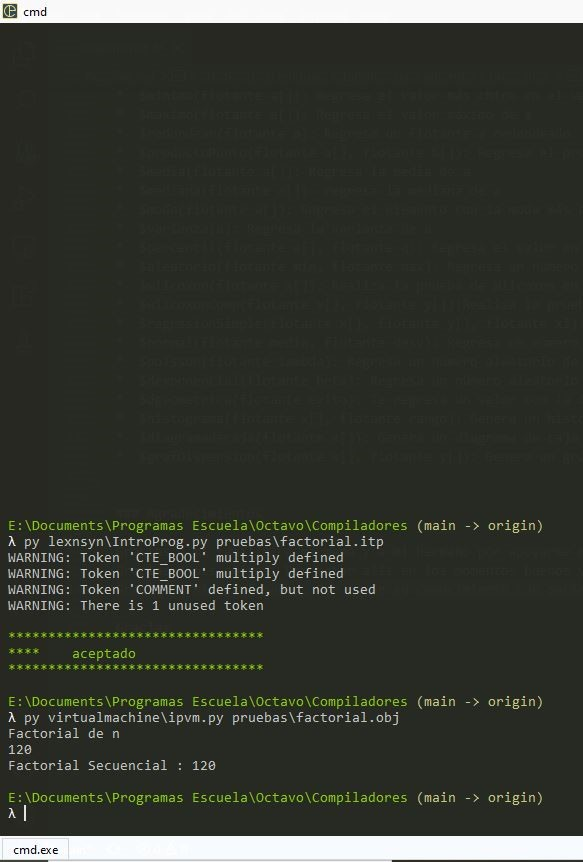
\includegraphics[scale=0.5]{chapters/chapter5/figures/FactorialCorriendo.JPG}
    \caption{El programa factorial compilado y ejecutado}
    \label{fig:my_label}
\end{figure}
\FloatBarrier

\section{Programa Fibonacci}

En este programa se implementaron dos formas para calcular el número n de la serie de Fibonacci. Una usando una función recursiva y la otra usando un método secuencial.
A continuación, se presenta el código fuente:
\begin{figure}[htbp]
    \centering
    \begin{lstlisting}
        programa fibbo { 
    	funcion entero fibbo(entero n){}{
    		si(n == 0){
    			regresar 0;
    		}
    		si(n == 1){
    			regresar 1;
    		}
    		regresar $fibbo(n-1) + $fibbo(n-2);
    	}
    	principal funcion {
    		entero pri,seg,ter,obj,aux;
    	} {	
    		obj = 8;
    		imprimir("fibbo ",$fibbo(obj));
    
    		pri = 0;
    		seg = 1;
    		aux = 1;
    		mientras( aux < obj){
    			ter = pri + seg;
    			pri = seg;
    			seg = ter;
    			aux = aux + 1;
    		}
    		imprimir("Fibbo secuencial : ",ter);
    
    	} 
}

    \end{lstlisting}
    \caption{Código fuente del programa fibbo}
    \label{fig:my_label}
\end{figure}
\FloatBarrier

A continuación se muestra su ejecución en consola:
\begin{figure}[htbp]
    \centering
    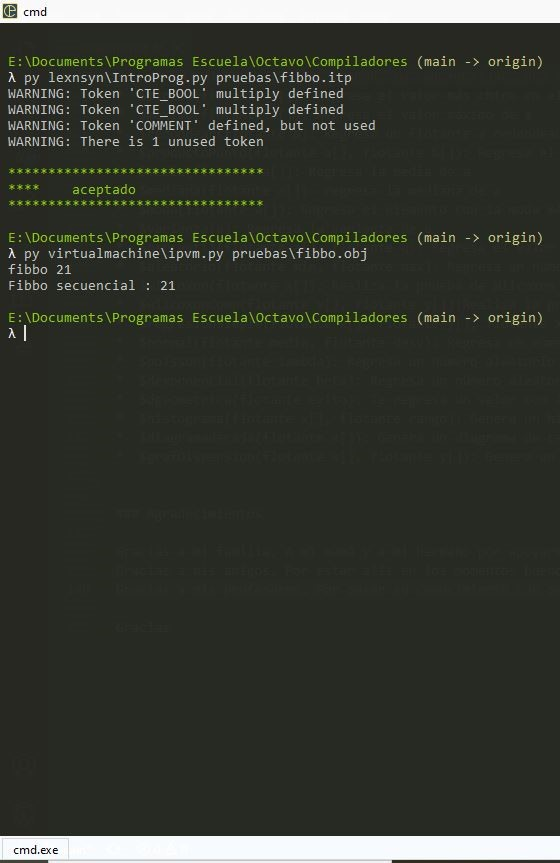
\includegraphics[scale=0.5]{chapters/chapter5/figures/fibbocorriendo.JPG}
    \caption{El programa fibbo compilado y ejecutado}
    \label{fig:my_label}
\end{figure}
\FloatBarrier


\section{Programa Busqueda y organización de arreglo}

En este programa se implementaron una función de búsqueda en un arreglo y un Bubble Sort para organizar un arreglo.
A continuación, se presenta el código fuente:
\begin{figure}[htbp]
    \centering
    \tiny
    \begin{lstlisting}
        programa arraysearchnsort{
            entero a[10];
            funcion vacio imprimirArr(entero a[10]){
                entero x;
            }{
                por(x = 0; x < 10; x = x+1;){
                    imprimir("a[",x,"] = ",a[x]);
                }
            }
        
            funcion vacio encontrar(entero x, entero a[10]){
                entero i,aux,aux2;
                bool loEncontre;
            }{
                imprimir("\n------------------\nBuscando ",x," en el arreglo :");
                $imprimirArr(a);
                imprimir("\n\n");
                aux = -1;
                loEncontre = falso;
                por(i = 0;i < 10;i = i +1;){
                    si(a[i] == x){
                        
                        aux2 = i;
                        i = 10+1;
                        loEncontre = verdadero;
                    }
                }
                si (loEncontre){
                    imprimir("Encontro ",x," en a[",aux2,"]");
                }sino{
                    imprimir("No se encontro el numero");
                }
            }
            principal funcion {
                entero i, j, aux;
            } {
                
                a = [1,5,4,3,2,-7,9,8,6,10];
                $encontrar(4,a);
                $encontrar(-1,a);
                imprimir("Desordenado:\n");
                $imprimirArr(a);
                por(i = 0; i < 10; i = i+1;){
                    por(j = 0; j < 10 -i-1; j = j+1;){
                        si(a[j] > a[j+1]){
                            aux = a[j];
                            a[j] = a[j+1];
                            a[j+1] = aux;
                        }
                    }
                }
                imprimir("\n\nOrdenado:\n");
                $imprimirArr(a);
                imprimir();
            }
        }
    \end{lstlisting}
    \caption{Código fuente del programa arraysearchnsort}
    \label{fig:my_label}
\end{figure}
\FloatBarrier
A continuación se muestra su ejecución en consola:
\begin{figure}[htbp]
    \centering
    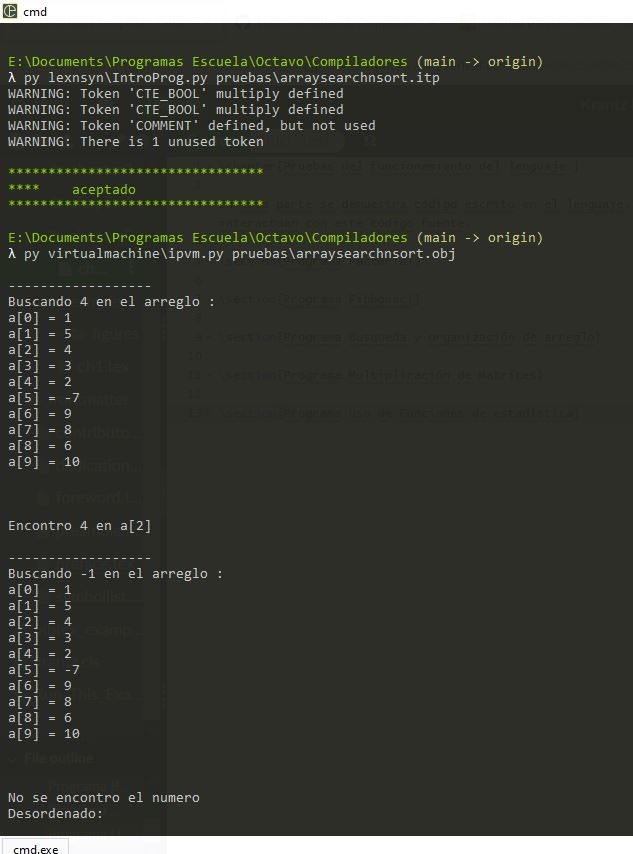
\includegraphics[scale=0.5]{chapters/chapter5/figures/arraycorriendo1.JPG}
    \caption{El Búsqueda y Sort compilado y ejecutado parte 1}
    \label{fig:my_label}
\end{figure}
\FloatBarrier
\begin{figure}[htbp]
    \centering
    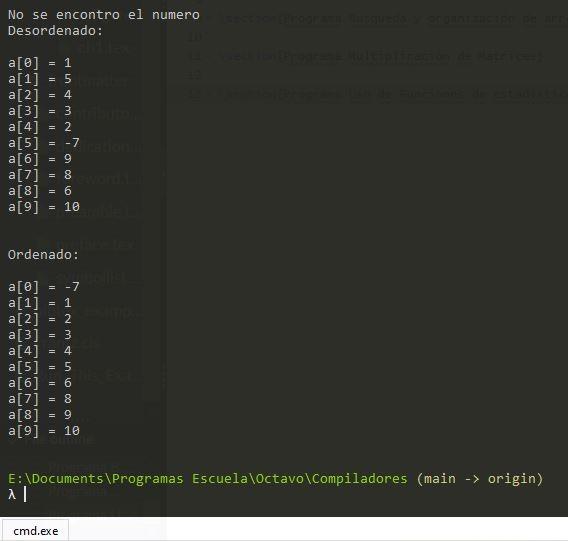
\includegraphics[scale=0.5]{chapters/chapter5/figures/arraycorriendo2.JPG}
    \caption{El Búsqueda y Sort compilado y ejecutado parte 2}
    \label{fig:my_label}
\end{figure}
\FloatBarrier

\section{Programa Multiplicación de Matrices}
En este programa se implemento una función de multiplicación de matrices.
A continuación, se presenta el código fuente:
\begin{figure}[htbp]
    \centering
    \tiny
    \begin{lstlisting}
        programa matmul{
            entero matA[2][3];
            entero matB[3][4];
            entero r1, comun ,c2;
            funcion vacio imprimirMatA(entero a[2][3]){
                entero x,y;
            }{
                por(x = 0; x < 2; x = x+1;){
                    por(y = 0; y < 3; y = y+1;){
                        imprimir("mat[",x ,"][", y,"] = ",a[x][y]);
                    }
                }
                
            }
            funcion vacio imprimirMatB(entero a[3][4]){
                entero x,y;
            }{
                por(x = 0; x < 3; x = x+1;){
                    por(y = 0; y < 4; y = y+1;){
                        imprimir("mat[",x ,"][", y,"] = ",a[x][y]);
                    }
                }
                
            }
        
            funcion vacio imprimirMat(entero a[2][4]){
                entero x,y;
            }{
                por(x = 0; x < 2; x = x+1;){
                    por(y = 0; y < 4; y = y+1;){
                        imprimir("mat[",x ,"][", y,"] = ",a[x][y]);
                    }
                }
                
            }
        
            principal funcion{
                entero matR[2][4];
                entero i,j,k;
            }{
                r1 = 2;
                comun = 3;
                c2 = 4;
                matA = [[1,2,3],[4,5,6]];
                imprimir("Matriz A :");
                $imprimirMatA(matA);
                matB = [[1,2,3,4],[5,6,7,8],[9,10,11,12]];
                imprimir("Matriz B :");
                $imprimirMatB(matB);
                
                por (i = 0; i < r1; i = i+1;) { //Iterar sobre los renglones de la primera matriz
                    por(j = 0; j < c2; j = j +1;){// Iterar sobre las columnas de la segunda matriz
                        matR[i][j] = 0;
                        por(k = 0; k < comun; k = k+1;){ 
                        // Recorer la col/reg para  hacer la multiplicacion
                            matR[i][j] = matR[i][j] + matA[i][k] * matB[k][j]; 
                            //matR[i][j] + matA[R_i][k] * matB[k][C_j]
                        }
                         
                    }
                }
        
                imprimir("Matriz R :");
                $imprimirMat(matR);
            }
        }
    \end{lstlisting}
    \caption{Código fuente del programa matmul}
    \label{fig:my_label}
\end{figure}
\FloatBarrier
A continuación se muestra su ejecución en consola:
\begin{figure}[htbp]
    \centering
    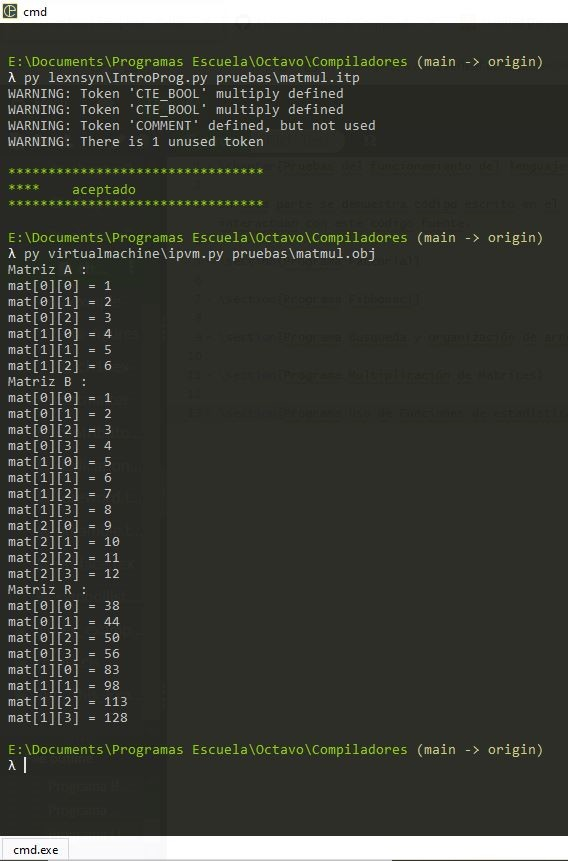
\includegraphics[scale=0.5]{chapters/chapter5/figures/matmulcorriendo.JPG}
    \caption{El matmul compilado y ejecutado}
    \label{fig:my_label}
\end{figure}
\FloatBarrier
\section{Programa Uso de Funciones de estadística}

En este programa se implementaron unas pruebas de Wilcoxon. Se crearon tres arreglos que simulaban muestras las cuales se popularon con números aleatorios pertenecientes a una distribución y se desplego la información básica de cada arreglo. Al final se hicieron unas pruebas  de wilcoxon para probar cual de las muestras se acomodaba mejor.

A continuación, se presenta el código fuente:
\begin{figure}[htbp]
    \centering
    \tiny
    \begin{lstlisting}
        programa pruebasDeWilcoxon{
                // La declaracion de variables
                flotante muestra1[100];
                flotante muestra2[100];
                // Declaracion de funciones
                funcion vacio imprimirDatos( flotante arr[100] ){
                    flotante prom, mod, med;
                }{
                    prom = $media(arr);
                    mod = $moda(arr);
                    med = $mediana(arr);
                    imprimir(" La media de esta distribucion es : ", prom);
                    imprimir(" La mediana de esta distribucion es : ", med);
                    imprimir(" La moda de esta distribucion es : ", mod);
                    imprimir(" El cuartil del 50 de los datos : ", $percentil(arr,50));
                }
                //Funcion principal
                principal funcion {
                    flotante muestra3[100];
                    entero i;
                    flotante p;
                }{
                    por(i = 0; i < 100; i = i+1;){
                        muestra1[i] = $normal(3.5,0.6);
                        muestra2[i] = $dexponencial(4);
                        muestra3[i] = $poisson(2);
                    }
            
                    imprimir("Muestra 1 : Normal");
                    $imprimirDatos(muestra1);
                    imprimir("Muestra 2 : Exponencial");
                    $imprimirDatos(muestra2);
                    imprimir("Muestra 3 : Poisson");
                    $imprimirDatos(muestra3);
            
                    //Pasar una prueba de wilcoxon p > 0.5
                    p = $wilcoxonComp(muestra1,muestra2);
                    imprimir("\n\nMuestra 1 v Muestra 2");
                    si(p > 0.5){
                        imprimir("Muestra 1 es la que mejor representa los datos");
                    }sino{
                        imprimir("Muestra 2 es la que mejor representa los datos");
                    }
            
                    p = $wilcoxonComp(muestra1,muestra3);
                    imprimir("\n\nMuestra 1 v Muestra 3");
                    si(p > 0.5){
                        imprimir("Muestra 1 es la que mejor representa los datos");
                    }sino{
                        imprimir("Muestra 3 es la que mejor representa los datos");
                    }
            
                    p = $wilcoxonComp(muestra3,muestra2);
                    imprimir("\n\nMuestra 3 v Muestra 2");
                    si(p > 0.5){
                        imprimir("Muestra 3 es la que mejor representa los datos");
                    }sino{
                        imprimir("Muestra 2 es la que mejor representa los datos");
                    }
            
                }
            
        }
    \end{lstlisting}
    \caption{Código fuente del programa}
    \label{fig:my_label}
\end{figure}
\FloatBarrier
A continuación se muestra su ejecución en consola:
\begin{figure}[htbp]
    \centering
    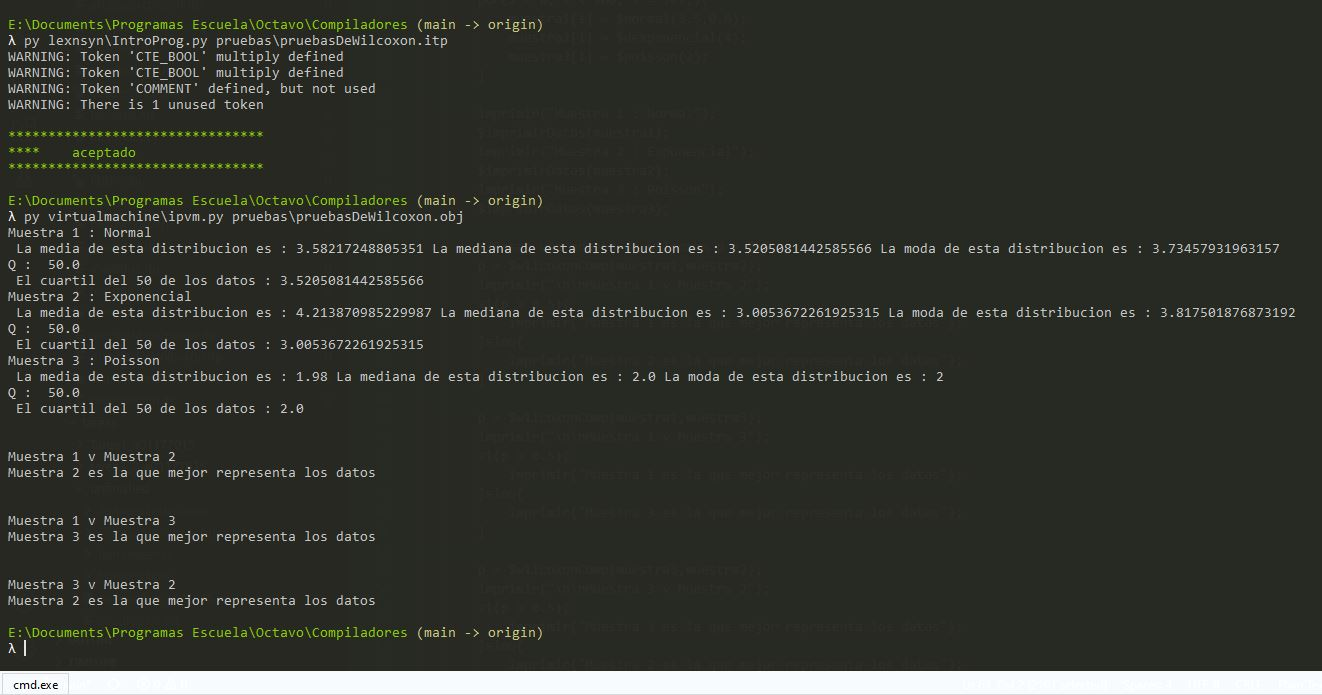
\includegraphics[scale=0.4]{chapters/chapter5/figures/wilcoxCorriendo.JPG}
    \caption{El programa de pruebasDeWilcoxon compilado y ejecutado}
    \label{fig:my_label}
\end{figure}

\part{Manual de Usuario}
\section{Introducción}

IntroProg es un lenguaje de programación diseñado para principiantes que quieran aprender a programar con lenguajes estilo C/C++ experimentando con funciones estadísticas.

\section{Herramientas que utiliza}
IntroProg se logró hacer con la ayuda de las siguientes herramientas:
\begin{itemize}
\item Python
\item Ply
\item SciPy
\item NumPy
\item MatPlotLib
\end{itemize}
\section{Requerimientos}

Para poder utilizar el lenguaje lo único que se requiere es tener Python instalado con las librerías que se mencionaron en las herramientas.

\section{Como correr un programa IntroProg}

Para correr tu programa IntroProg debes de primero compilarlo con el archivo de IntroProg.py que se encuentra dentro de la carpeta lexnsyn
\begin{lstlisting}
py IntroProg.py camino/a/tu/archivo
\end{lstlisting}

Esto generara un archivo obj el cual la máquina virtual que está en la carpeta de virtualmachine va a usar para ejecutar tu código

\begin{lstlisting}
py itvm.py camino/a/tu/archivo/obj
\end{lstlisting}

\section{Como utilizar el lenguaje}

Para poder utilizar el lenguaje lo primero que debes de hacer es crear un archivo itp. Este archivo deberá contener tu código fuente que vayas creando.
Los archivos itp siguen la siguiente estructura:
\begin{lstlisting}

programa pelos{
    //Primero deben de ir la declaracion de variables globales
    //Luego deben de ir las declaracion de tus funciones
    //Luego va la función principal
    principal funcion{}{
        imprimir("¡¡Hola Mundo!!");
    }

}

\end{lstlisting}

Los tipos que utiliza IntroProg para sus variables son los siguientes:
\begin{itemize}
    \item Enteros
    \item Flotantes
    \item Caracteres (char)
    \item Booleanos (bool)
\end{itemize}

Para la declaración de una variable basta con escribir el tipo de la variable seguido por el nombre de la variable. Este nombre puede ser cualquier combinación de letras, números y guiones bajos (\_) que empiezen con una letra.

\begin{lstlisting}
    entero num;
    flotante num2;
    char letra;
    bool booleano1;
\end{lstlisting}

\section{Operaciones}

Para realizar operaciones con IntroProg basta con escribirlas como si fueran operaciones matemáticas.
\begin{lstlisting}
    // suma
    num = 1+1;
    // resta
    num = num -1;
    // multiplicacion
    num2 = num \item 20;
    // Division
    num2 = num /num2;
    // Tambien se pueden usar parentesis
    num2 = (1+1)\itemnum - num2 \item num2;
    // Taqmbién puedes hacer funciones relacionales y lógicas
    booleano1 = num2 > 1 || (num2 == num && num <> 1); 
\end{lstlisting}

\section{Funciones}

 Para construir funciones en IntroProg debes de seguir la siguiente estructura:

\begin{lstlisting}
  funcion tipo nombre(parametros){
      //Declaraciones
      // Se puede dejar vacio si no se usan variables locales
    }{
        //Tu asmbroso codigo
    }
\end{lstlisting}

Recuerda que puedes tener funciones que no tengan parámetros y no regresen nada

\begin{lstlisting}
    funcion vacia hola(){}{
        imprimir("Hola!!");
    }
\end{lstlisting}

O funciones que puedan hacer operaciones y que te regresen un valor
\begin{lstlisting}
    funcion entera sumaMagica(entero a, entero b){
        entero ingredienteSecreto;
    }{
        ingredienteSecreto = 1000;
        regresar a + b\itemingredienteSecreto;
    }
\end{lstlisting}
Y para utilizar tus funciones solo basta con escribir un \$ seguido por el nombre de tu función y sus parametros entre paréntesis

\begin{lstlisting}
    \$hola();
    num = \$sumaMagica(1,2);
\end{lstlisting}

\section{Funciones especiales}

IntroProg también te provee una lista de funciones que puedes utilizar para tu código
\begin{itemize}
    \item  \$leer() : Regresa la lectura capturada de consola
    \item  \$modulo(flotante a, flotante b): Regresa el resultado de a\%b
    \item  \$suma(flotante a[]): Suma todos los elementos de un arreglo y regresa sus resultados
    \item  \$raiz(flotante a): Regresa el flotante resultante de la raíz de a
    \item  \$exp(flotante a): Regresa la exponencial de e\^a
    \item  \$elevar(flotante a, flotante b): Regresa el resultado de a\^b
    \item  \$techo(flotante a): Regresa un flotante a redondeado para arriba
    \item  \$piso(flotante a): Regresa un flotante a redondeado para abajo
    \item  \$cos(flotante a): Regresa el coseno de a
    \item  \$sen(flotante a): Regresa el seno de a
    \item  \$tan(flotante a): Regresa la tangente de a
    \item  \$cotan(flotante a): Regresa la cotangente de a
    \item  \$sec(flotante a): Regresa la secante de a
    \item  \$cosec(flotante a): Regresa la cosecante de a
    \item  \$log(flotante a): Regresa el logaritmo natural de a
    \item  \$minimo(flotante a[]): Regresa el valor más chico en el vector a
    \item  \$maximo(flotante a[]): Regresa el valor máximo de a
    \item  \$redondear(flotante a): Regresa un flotante a redondeado
    \item  \$productoPunto(flotante a[], flotante b[]): Regresa el producto punto entre los vectores de entrada a y b
    \item  \$media(flotante a[]): Regresa la media de a
    \item  \$mediana(flotante a[]): regresa la mediana de a
    \item  \$moda(flotante a[]): Regresa el elemento con la moda más alta de a
    \item  \$varianza(a): Regresa la varianza de a
    \item  \$percentil(flotante a[], flotante q): Regresa el valor en el que se encuentran q% de los valores en a
    \item  \$aleatorio(flotante min, flotante max): Regresa un número flotante aleatorio entre los rangos de argumentos mínimos y máximos
    \item  \$wilcoxon(flotante x[]): Realiza la prueba de Wilcoxon en la serie de datos en x
    \item  \$wilcoxonComp(flotante x[], flotante y[]):Realiza la prueba de Wilcoxon se realiza la prueba sobre los datos x y y
    \item  \$regresionSimple(flotante x[], flotante y[], flotante xi): Dado un set de x y y se usará regresión lineal simple para encontrar f(xi) y se regresara ese valor
    \item  \$normal(flotante media, flotante desv): Regresa un número escalar que pertenezca a la distribución normal dado los parámetros
    \item  \$poisson(flotante lambda): Regresa un número aleatorio de la distribución Poisson con la lambda dada
    \item  \$dexponencial(flotante beta): Regresa un número aleatorio de la distribución Exponencial correspondiente a la beta (o 1/Lambda) dada
    \item  \$dgeometrica(flotante exito): Te regresa un valor con la distribución geométrica con la probabilidad de exito dada
    \item  \$histograma(flotante x[], flotante rango): Genera un histograma a partir de los datos en el vector de x con un rango entre los datos de rango
    \item  \$diagramadecaja(flotante x[]): Genera un diagrama de caja y bigotes de los datos en en x
    \item  \$grafDispersion(flotante x[], flotante y[]): Genera un gráfico de dispersión con los valores de ‘x’ y ‘y’

\end{itemize}


\part{Ejemplos de Documentación en código}

Ejemplo de funciones documentadas en el compilador:
\scriptsize
\begin{minted}{python}
    # Func : getArrayData
    # Params : Una dirección Virtual addr
    # ret : La información de las dimensiones de un arreglo
    # Desc : Regresa la información de las dimensiones de un arreglo
    def getArrayData(addr):
        global dirfunc
        global currscope
        res = {}
    
        for var in dirfunc[currscope]['vartab'].values():
    
            if addr['address'] == var['address']:
                res['size'] = var['size']
                res['dimlen'] = var['dimlen']
                res['dims'] = var['dims']
                return res
        for var in dirfunc['global']['vartab'].values():
    
            if addr['address'] == var['address']:
    
                res['size'] = var['size']
                res['dimlen'] = var['dimlen']
                res['dims'] = var['dims']
                return res
        return res
    
   
\end{minted}
\scriptsize
\begin{minted}{python}
# Func : addConst
# Param : Una constante cte, un tipo tipo y la linea del token line
# Desc : Agrega una constante a la tabla de constante y le asigna una dirección 
# virtual de acuerdo al tipo de la constante.

def addConst(cte,tipo,line):
    # Rango de memoria constantes
    global constint
    global constfloat
    global constchar
    global constbool
    global conststring
    # Contadores constantes
    global cteintcount
    global ctefloatcount
    global ctecharcount
    global cteboolcount
    global ctestringcount
    # Maximos de variables
    global INTMAX
    global FLOATMAX
    global CHARMAX
    global BOOLMAX
    global STRINGMAX
    #Tabla const
    global ctetab
    global objctetab

    # Si la llave no es un string hacer una llave string
    if type(cte) is not str:
        ctkey = str(cte)
    else:
        ctkey = cte
    # Agregarla de acuerdo al tipo y con su dirección de memoria adecuada
    if tipo == 'entero':
        if cteintcount < INTMAX:
            ctetab[ctkey] = constint + cteintcount
            objctetab[ctetab[ctkey]] = cte
            cteintcount += 1
            return ctetab[ctkey]
        else:
            printerror(
                "Error de Semantica: sobrepaso el limite de constantes declaradas en la linea %r" % (line))
    elif tipo == 'flotante':
        if ctefloatcount < FLOATMAX:
            ctetab[ctkey] = constfloat + ctefloatcount
            objctetab[ctetab[ctkey]] = cte
            ctefloatcount += 1
            return ctetab[ctkey]
        else:
            printerror(
                "Error de Semantica: sobrepaso el limite de constantes declaradas en la linea %r" % (line))
    elif tipo == 'char':
        if ctecharcount < CHARMAX:
            ctetab[cte] = constchar + ctecharcount
            objctetab[ctetab[cte]] = cte
            ctecharcount += 1
            return ctetab[ctkey]
        else:

            printerror(
                "Error de Semantica: sobrepaso el limite de constantes declaradas en la linea %r" % (line))
    elif tipo == 'bool':
        if cteboolcount < BOOLMAX:
            ctetab[cte] = constbool + cteboolcount
            if cte == 'verdadero':
                objctetab[ctetab[cte]] = True
            else:
                objctetab[ctetab[cte]] = False
            cteboolcount += 1
            return ctetab[ctkey]
        else:
            printerror(
                "Error de Semantica: sobrepaso el limite de constantes declaradas en la linea %r" % (line))
    elif tipo == 'cadena':
        if ctestringcount < STRINGMAX:
            ctetab[ctkey] = conststring + ctestringcount
            objctetab[ctetab[ctkey]] = cte
            ctestringcount += 1
            return ctetab[ctkey]
        else:

            printerror(
                "Error de Semantica: sobrepaso el limite de constantes declaradas en la linea %r" % (line))

# Func : assignvirtualaddress
# Params : Una tabla de variables vartab, un scope addresscope y el número del linea de los tokens linenum
# Ret : Una tabla de variables actualizada con las direcciones de cada variable
# Desc : Asigna las direcciones virtuales a la tabla de variables
def assignvirtualaddress(vartab,addressscope,linenum):
    # Rangos globales de memoria
    global globalint
    global globalfloat
    global globalchar
    global globalbool
    global globalpoint
    # Direcciones locales
    global localint
    global localfloat
    global localchar
    global localbool
    global localpoint
    # Cant. Maximas de variables
    global INTMAX
    global FLOATMAX
    global CHARMAX
    global BOOLMAX
    global POINTAYMAX

    # Contadores globales
    global glbintcount
    global glbfloatcount
    global glbcharcount
    global glbboolcount
    #
    # Contadores de variables
    intcount = 0
    floatcount = 0
    charcount = 0
    boolcount = 0

    # Contadores de arreglos
    pointcount = 0

    if addressscope == 'global':
        for k in vartab.keys():
            if('dims' in vartab[k].keys()): # Asignacion de direcciones de arreglos
                incr = vartab[k]['size']
                isArr = True
            else:
                incr = 1
                isArr = False


            if(vartab[k]['tipo'] == 'entero'): #Asignar las direcciones enteras
                if (intcount < INTMAX):
                    vartab[k]['address'] = globalint + intcount
                    intcount += incr
                    if isArr:
                        addConst(vartab[k]['address'], 'entero', linenum)
                else:
                    printerror("Error de Semantica: sobrepaso el limite de variables declaradas en la linea %r" % (linenum))

            elif (vartab[k]['tipo'] == 'flotante'):#Asignar las direcciones flotantes
                if (floatcount < FLOATMAX):
                    vartab[k]['address'] = globalfloat + floatcount
                    floatcount += incr
                    if isArr:
                        addConst(vartab[k]['address'], 'entero', linenum)
                else:
                    printerror("Error de Semantica: sobrepaso el limite de variables declaradas en la linea %r" % (linenum))

            elif (vartab[k]['tipo'] == 'char'):#Asignar las direcciones char
                if (charcount < CHARMAX):
                    vartab[k]['address'] = globalchar + charcount
                    charcount += incr
                    if isArr:
                        addConst(vartab[k]['address'], 'entero', linenum)
                else:
                    printerror("Error de Semantica: sobrepaso el limite de variables declaradas en la linea %r" % (linenum))
            elif (vartab[k]['tipo'] == 'bool'):#Asignar las direcciones char
                if (boolcount < BOOLMAX):
                    vartab[k]['address'] = globalbool + boolcount
                    boolcount += incr
                else:
                    printerror("Error de Semantica: sobrepaso el limite de variables declaradas en la linea %r" % (linenum))
    elif addressscope == 'local':
        for k in vartab.keys():
            if('dims' in vartab[k].keys()): # Asignacion de direcciones de arreglos
                incr = vartab[k]['size']
                isArr = True
            else:
                incr = 1
                isArr = False

            if(vartab[k]['tipo'] == 'entero'): #Asignar las direcciones enteras
                if (intcount < INTMAX):
                    vartab[k]['address'] = localint + intcount
                    intcount += incr
                    if isArr:
                        addConst(vartab[k]['address'], 'entero', linenum)
                else:
                    printerror("Error de Semantica: sobrepaso el limite de variables declaradas en la linea %r" % (linenum))

            elif (vartab[k]['tipo'] == 'flotante'):#Asignar las direcciones flotantes
                if (floatcount < FLOATMAX):
                    vartab[k]['address'] = localfloat + floatcount
                    floatcount += incr
                    if isArr:
                        addConst(vartab[k]['address'], 'entero', linenum)
                else:
                    printerror("Error de Semantica: sobrepaso el limite de variables declaradas en la linea %r" % (linenum))

            elif (vartab[k]['tipo'] == 'char'):#Asignar las direcciones char
                if (charcount < CHARMAX):
                    vartab[k]['address'] = localchar + charcount
                    if isArr:
                        addConst(vartab[k]['address'], 'entero', linenum)
                    charcount += incr
                else:
                    printerror("Error de Semantica: sobrepaso el limite de variables declaradas en la linea %r" % (linenum))
            elif (vartab[k]['tipo'] == 'bool'):#Asignar las direcciones char
                if (boolcount < BOOLMAX):
                    vartab[k]['address'] = localbool + boolcount
                    if isArr:
                        addConst(vartab[k]['address'], 'entero', linenum)
                    boolcount += incr
                else:
                    printerror(
                    "Error de Semantica: sobrepaso el limite de variables declaradas en la linea %r" % (linenum)
                    )
    return vartab, intcount, floatcount, charcount, boolcount


\end{minted}

\newpage
Ejemplos de Documentación en la máquina virtual:
\scriptsize
\begin{minted}{python}
    
    
    # Func: storeinmem
    # Param: Una direccion virtual addrs, un valor val, y opcionalmente un flag indicando 
    # si guardar en la variable temporal era
    # Desc: Guardar en memoria el valor dado.
    def storeinmem(addrs,val, isera = False):
        scop, atype, aoff = getTypeAndOffset(addrs)
        if scop == 'global':
            if atype == 0: #entero
                globmem.mint[aoff] = val
            elif atype == 1: #float
                globmem.mfloat[aoff] = val
            elif atype == 2: #char
                globmem.mchar[aoff] = val
            elif atype == 3: #bool
                globmem.mbool[aoff] = val
            elif atype == 4: #pointer
                globmem.mpoint[aoff] = val
        elif scop == 'local':
            if atype == 0: #entero
                if isera:
                    eratemp[0].mint[aoff] = val
                else:
                    memstack[-1][0].mint[aoff] = val
            elif atype == 1: #float
                if isera:
                    eratemp[0].mfloat[aoff] = val
                else:
                    memstack[-1][0].mfloat[aoff] = val
            elif atype == 2: #char
                if isera:
                    eratemp[0].mchar[aoff] = val
                else:
                    memstack[-1][0].mchar[aoff] = val
            elif atype == 3: #bool
                if isera:
                    eratemp[0].mbool[aoff] = val
                else:
                    memstack[-1][0].mbool[aoff] = val
            elif atype == 4: #pointer
                if isera:
                    eratemp[0].mpoint[aoff] = val
                else:
                    memstack[-1][0].mpoint[aoff] = val
        elif scop == 'temp':
            if atype == 0: #entero
                if isera:
                    eratemp[1].mint[aoff] = val
                else:
                    memstack[-1][1].mint[aoff] = val
            elif atype == 1: #float
                if isera:
                    eratemp[1].mfloat[aoff] = val
                else:
                    memstack[-1][1].mfloat[aoff] = val
            elif atype == 2: #char
                if isera:
                    eratemp[1].mchar[aoff] = val
                else:
                    memstack[-1][1].mchar[aoff] = val
            elif atype == 3: #bool
                if isera:
                    eratemp[1].mbool[aoff] = val
                else:
                    memstack[-1][1].mbool[aoff] = val
            elif atype == 4: #pointer
                if isera:
                    if eratemp[1].mpoint[aoff] == None:
                        eratemp[1].mpoint[aoff] = val
                    else:
                        
                        storeinmem(eratemp[1].mpoint[aoff],val,isera)
                else:
                    
                    if memstack[-1][1].mpoint[aoff] == None:
                        memstack[-1][1].mpoint[aoff] = val
                        
                    else:
                        #val, _ = getexpoper(memstack[-1][1].mpoint[aoff])
                        
                        storeinmem(memstack[-1][1].mpoint[aoff],val)
                        
                        
    # Func: valtonum
    # params: Un valor val, y un tipo t
    # ret: Regresa el valor de v como el tipo t
    # Desc: Cambiar valor a numero si es necesario
    def valtonum(val,t):
        if t == 2:
            val = ord(val)
        elif t == 3:
            if val:
                val = 1
            else:
                val = 0
        return val
    
    
    # Func: reusePointer
    # Params: Una dirección virtual addrs y un valor 
    # Reescribir el valor del apuntador cuando es necesario
    def reusePointer(addrs,val):
        scop, atype, aoff = getTypeAndOffset(addrs)
        memstack[-1][1].mpoint[aoff] = val
    
    
    # Func : exeExpresion
    # Params : Un operador op, tres direcciones virtuals ladd, radd resadd
    # Desc : Ejecuta la acción del cuadruplo y la guarda en memoria
    def exeExpresion(op,ladd,radd,resadd):
        lop,lt = getexpoper(ladd)
        rop,rt = getexpoper(radd)
        if lop == None or rop == None:
            printerr(
            'Esta intentando realizar operaciónes con variables que no cuentan con un valor.'
            +
            '\nRevisa el códgo para asegurar que no haya alguna variable sin valor en alguna de tus operaciones'
            ,ip)
        lop = valtonum(lop,lt)
        rop = valtonum(rop,rt)
        aux = 0
        # Operadores ['*','/','+','-','>','<','>=','<=','!=','==','||','&&']
        if op == '*': 
            # Multiplicacion
            aux = lop * rop
    
        elif op == '/': 
            # Division
            aux = lop / rop
    
        elif op == '+': 
            #Suma 
            if rop == '':
                aux = abs(lop)
            else:
                aux = lop + rop
    
        elif op == '-': 
            #Resta
            if rop == '':
                aux = -1 * abs(lop)
            else:
                aux = lop - rop
    
        elif op == '>': 
            #Mayorque
            aux = lop > rop
    
        elif op == '<':
            #menor que
            aux = lop < rop
    
        elif op == '>=': 
            # mayor igual
            aux = lop >= rop
    
        elif op == '<=': 
            #menor igual
            aux = lop <= rop
    
        elif op == '==': 
            #igual (relacional)
            aux = lop == rop
    
        elif op == '!=': 
            #diferente
            aux = lop != rop
    
        elif op == '&&': 
            # and
            aux = lop and rop
    
        elif op == '||': 
            # or
            aux = lop or rop
        if type(resadd) is str: # Reescribir el pointer en caso de ser necesaria
            reusePointer(int(resadd[1:]),aux)
        else:
            storeinmem(resadd,aux)
\end{minted}

%\bibliographystyle{plain}
%\bibliography{bibtex_example}

\printindex

\end{document}
